\documentclass[twoside]{book}

% Packages required by doxygen
\usepackage{fixltx2e}
\usepackage{calc}
\usepackage{doxygen}
\usepackage[export]{adjustbox} % also loads graphicx
\usepackage{graphicx}
\usepackage[utf8]{inputenc}
\usepackage{makeidx}
\usepackage{multicol}
\usepackage{multirow}
\PassOptionsToPackage{warn}{textcomp}
\usepackage{textcomp}
\usepackage[nointegrals]{wasysym}
\usepackage[table]{xcolor}

% Font selection
\usepackage[T1]{fontenc}
\usepackage[scaled=.90]{helvet}
\usepackage{courier}
\usepackage{amssymb}
\usepackage{sectsty}
\renewcommand{\familydefault}{\sfdefault}
\allsectionsfont{%
  \fontseries{bc}\selectfont%
  \color{darkgray}%
}
\renewcommand{\DoxyLabelFont}{%
  \fontseries{bc}\selectfont%
  \color{darkgray}%
}
\newcommand{\+}{\discretionary{\mbox{\scriptsize$\hookleftarrow$}}{}{}}

% Page & text layout
\usepackage{geometry}
\geometry{%
  a4paper,%
  top=2.5cm,%
  bottom=2.5cm,%
  left=2.5cm,%
  right=2.5cm%
}
\tolerance=750
\hfuzz=15pt
\hbadness=750
\setlength{\emergencystretch}{15pt}
\setlength{\parindent}{0cm}
\setlength{\parskip}{3ex plus 2ex minus 2ex}
\makeatletter
\renewcommand{\paragraph}{%
  \@startsection{paragraph}{4}{0ex}{-1.0ex}{1.0ex}{%
    \normalfont\normalsize\bfseries\SS@parafont%
  }%
}
\renewcommand{\subparagraph}{%
  \@startsection{subparagraph}{5}{0ex}{-1.0ex}{1.0ex}{%
    \normalfont\normalsize\bfseries\SS@subparafont%
  }%
}
\makeatother

% Headers & footers
\usepackage{fancyhdr}
\pagestyle{fancyplain}
\fancyhead[LE]{\fancyplain{}{\bfseries\thepage}}
\fancyhead[CE]{\fancyplain{}{}}
\fancyhead[RE]{\fancyplain{}{\bfseries\leftmark}}
\fancyhead[LO]{\fancyplain{}{\bfseries\rightmark}}
\fancyhead[CO]{\fancyplain{}{}}
\fancyhead[RO]{\fancyplain{}{\bfseries\thepage}}
\fancyfoot[LE]{\fancyplain{}{}}
\fancyfoot[CE]{\fancyplain{}{}}
\fancyfoot[RE]{\fancyplain{}{\bfseries\scriptsize Generated by Doxygen }}
\fancyfoot[LO]{\fancyplain{}{\bfseries\scriptsize Generated by Doxygen }}
\fancyfoot[CO]{\fancyplain{}{}}
\fancyfoot[RO]{\fancyplain{}{}}
\renewcommand{\footrulewidth}{0.4pt}
\renewcommand{\chaptermark}[1]{%
  \markboth{#1}{}%
}
\renewcommand{\sectionmark}[1]{%
  \markright{\thesection\ #1}%
}

% Indices & bibliography
\usepackage{natbib}
\usepackage[titles]{tocloft}
\setcounter{tocdepth}{3}
\setcounter{secnumdepth}{5}
\makeindex

% Packages requested by user
\usepackage{latexsym,amssymb,amsfonts,amsmath,amstext,myMacros}

% Hyperlinks (required, but should be loaded last)
\usepackage{ifpdf}
\ifpdf
  \usepackage[pdftex,pagebackref=true]{hyperref}
\else
  \usepackage[ps2pdf,pagebackref=true]{hyperref}
\fi
\hypersetup{%
  colorlinks=true,%
  linkcolor=blue,%
  citecolor=blue,%
  unicode%
}

% Custom commands
\newcommand{\clearemptydoublepage}{%
  \newpage{\pagestyle{empty}\cleardoublepage}%
}

\usepackage{caption}
\captionsetup{labelsep=space,justification=centering,font={bf},singlelinecheck=off,skip=4pt,position=top}

%===== C O N T E N T S =====

\begin{document}

% Titlepage & ToC
\hypersetup{pageanchor=false,
             bookmarksnumbered=true,
             pdfencoding=unicode
            }
\pagenumbering{roman}
\begin{titlepage}
\vspace*{7cm}
\begin{center}%
{\Large Modular Estimator }\\
\vspace*{1cm}
{\large Generated by Doxygen 1.8.11}\\
\end{center}
\end{titlepage}
\clearemptydoublepage
\tableofcontents
\clearemptydoublepage
\pagenumbering{arabic}
\hypersetup{pageanchor=true}

%--- Begin generated contents ---
\chapter{Namespace Index}
\section{Packages}
Here are the packages with brief descriptions (if available)\+:\begin{DoxyCompactList}
\item\contentsline{section}{\hyperlink{namespaceAttitudeSubstate}{Attitude\+Substate} \\*This package contains the \hyperlink{classAttitudeSubstate_1_1AttitudeState6DOF}{Attitude\+State6\+D\+OF} class }{\pageref{namespaceAttitudeSubstate}}{}
\item\contentsline{section}{\hyperlink{namespaceState}{State} \\*This package contains the \hyperlink{classState_1_1ModularFilter}{Modular\+Filter} class }{\pageref{namespaceState}}{}
\item\contentsline{section}{\hyperlink{namespaceSubStates}{Sub\+States} \\*This package contains the \hyperlink{classSubStates_1_1SubState}{Sub\+State} class }{\pageref{namespaceSubStates}}{}
\end{DoxyCompactList}

\chapter{Hierarchical Index}
\section{Class Hierarchy}
This inheritance list is sorted roughly, but not completely, alphabetically\+:\begin{DoxyCompactList}
\item \contentsline{section}{State.\+Modular\+Filter}{\pageref{classState_1_1ModularFilter}}{}
\item \contentsline{section}{Signals.\+Signal\+Source}{\pageref{classSignals_1_1SignalSource}}{}
\begin{DoxyCompactList}
\item \contentsline{section}{Signals.\+Point\+Source}{\pageref{classSignals_1_1PointSource}}{}
\begin{DoxyCompactList}
\item \contentsline{section}{Signals.\+Static\+X\+Ray\+Point\+Source}{\pageref{classSignals_1_1StaticXRayPointSource}}{}
\end{DoxyCompactList}
\item \contentsline{section}{Signals.\+Poisson\+Source}{\pageref{classSignals_1_1PoissonSource}}{}
\begin{DoxyCompactList}
\item \contentsline{section}{Signals.\+Periodic\+Poisson\+Source}{\pageref{classSignals_1_1PeriodicPoissonSource}}{}
\item \contentsline{section}{Signals.\+Static\+Poisson\+Source}{\pageref{classSignals_1_1StaticPoissonSource}}{}
\begin{DoxyCompactList}
\item \contentsline{section}{Signals.\+Static\+X\+Ray\+Point\+Source}{\pageref{classSignals_1_1StaticXRayPointSource}}{}
\item \contentsline{section}{Signals.\+Uniform\+Noise\+X\+Ray\+Source}{\pageref{classSignals_1_1UniformNoiseXRaySource}}{}
\end{DoxyCompactList}
\end{DoxyCompactList}
\end{DoxyCompactList}
\item A\+BC\begin{DoxyCompactList}
\item \contentsline{section}{Sub\+States.\+Sub\+State}{\pageref{classSubStates_1_1SubState}}{}
\begin{DoxyCompactList}
\item \contentsline{section}{Attitude\+Substate.\+Attitude\+State6\+D\+OF}{\pageref{classAttitudeSubstate_1_1AttitudeState6DOF}}{}
\item \contentsline{section}{Signal\+Correlation\+Substate.\+Correlation\+Filter}{\pageref{classSignalCorrelationSubstate_1_1CorrelationFilter}}{}
\end{DoxyCompactList}
\end{DoxyCompactList}
\end{DoxyCompactList}

\chapter{Class Index}
\section{Class List}
Here are the classes, structs, unions and interfaces with brief descriptions\+:\begin{DoxyCompactList}
\item\contentsline{section}{\hyperlink{classAttitudeSubstate_1_1AttitudeState6DOF}{Attitude\+Substate.\+Attitude\+State6\+D\+OF} \\*Estimates the attitude of a vehicle in three dimensions, along with three gyro bias states }{\pageref{classAttitudeSubstate_1_1AttitudeState6DOF}}{}
\item\contentsline{section}{\hyperlink{classSignalCorrelationSubstate_1_1CorrelationFilter}{Signal\+Correlation\+Substate.\+Correlation\+Filter} }{\pageref{classSignalCorrelationSubstate_1_1CorrelationFilter}}{}
\item\contentsline{section}{\hyperlink{classState_1_1ModularFilter}{State.\+Modular\+Filter} }{\pageref{classState_1_1ModularFilter}}{}
\item\contentsline{section}{\hyperlink{classSignals_1_1PointSource}{Signals.\+Point\+Source} }{\pageref{classSignals_1_1PointSource}}{}
\item\contentsline{section}{\hyperlink{classSignals_1_1PoissonSource}{Signals.\+Poisson\+Source} }{\pageref{classSignals_1_1PoissonSource}}{}
\item\contentsline{section}{\hyperlink{classSignals_1_1SignalSource}{Signals.\+Signal\+Source} }{\pageref{classSignals_1_1SignalSource}}{}
\item\contentsline{section}{\hyperlink{classSignals_1_1StaticPoissonSource}{Signals.\+Static\+Poisson\+Source} }{\pageref{classSignals_1_1StaticPoissonSource}}{}
\item\contentsline{section}{\hyperlink{classSignals_1_1StaticXRayPointSource}{Signals.\+Static\+X\+Ray\+Point\+Source} }{\pageref{classSignals_1_1StaticXRayPointSource}}{}
\item\contentsline{section}{\hyperlink{classSignals_1_1UniformNoiseXRaySource}{Signals.\+Uniform\+Noise\+X\+Ray\+Source} }{\pageref{classSignals_1_1UniformNoiseXRaySource}}{}
\end{DoxyCompactList}

\chapter{Namespace Documentation}
\hypertarget{namespaceAttitudeSubstate}{}\section{Attitude\+Substate Namespace Reference}
\label{namespaceAttitudeSubstate}\index{Attitude\+Substate@{Attitude\+Substate}}


This package contains the \hyperlink{classAttitudeSubstate_1_1AttitudeState6DOF}{Attitude\+State6\+D\+OF} class.  


\subsection*{Classes}
\begin{DoxyCompactItemize}
\item 
class \hyperlink{classAttitudeSubstate_1_1AttitudeState6DOF}{Attitude\+State6\+D\+OF}
\begin{DoxyCompactList}\small\item\em Estimates the attitude of a vehicle in three dimensions, along with three gyro bias states. \end{DoxyCompactList}\end{DoxyCompactItemize}


\subsection{Detailed Description}
This package contains the \hyperlink{classAttitudeSubstate_1_1AttitudeState6DOF}{Attitude\+State6\+D\+OF} class. 


\chapter{Class Documentation}
\hypertarget{classAttitudeSubstate_1_1AttitudeState6DOF}{}\section{Attitude\+Substate.\+Attitude\+State6\+D\+OF Class Reference}
\label{classAttitudeSubstate_1_1AttitudeState6DOF}\index{Attitude\+Substate.\+Attitude\+State6\+D\+OF@{Attitude\+Substate.\+Attitude\+State6\+D\+OF}}


Estimates the attitude of a vehicle in three dimensions, along with three gyro bias states.  




Inheritance diagram for Attitude\+Substate.\+Attitude\+State6\+D\+OF\+:
\nopagebreak
\begin{figure}[H]
\begin{center}
\leavevmode
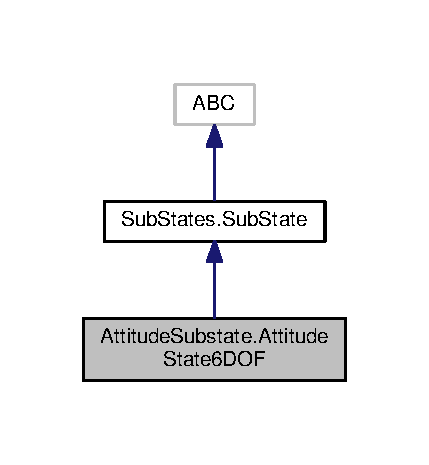
\includegraphics[width=206pt]{classAttitudeSubstate_1_1AttitudeState6DOF__inherit__graph}
\end{center}
\end{figure}


Collaboration diagram for Attitude\+Substate.\+Attitude\+State6\+D\+OF\+:
\nopagebreak
\begin{figure}[H]
\begin{center}
\leavevmode
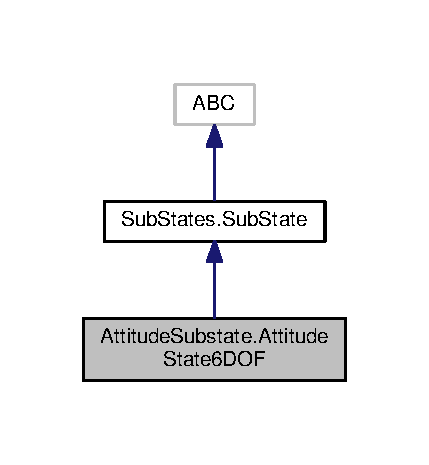
\includegraphics[width=206pt]{classAttitudeSubstate_1_1AttitudeState6DOF__coll__graph}
\end{center}
\end{figure}
\subsection*{Public Member Functions}
\begin{DoxyCompactItemize}
\item 
def \hyperlink{classAttitudeSubstate_1_1AttitudeState6DOF_a337e9fa07d0211f86b359e5d9deee1b8}{\+\_\+\+\_\+init\+\_\+\+\_\+} (self, attitude\+Quaternion=Quaternion(\mbox{[}1, 0, 0, 0\mbox{]}), attitude\+Error\+Covariance=np.\+eye(3), gyro\+Bias=np.\+zeros(3), gyro\+Bias\+Covariance=np.\+eye(3), t=0)
\begin{DoxyCompactList}\small\item\em {\bfseries init} \end{DoxyCompactList}\item 
def \hyperlink{classAttitudeSubstate_1_1AttitudeState6DOF_a8e420e4a7806669c1286a1a70ce019da}{get\+State\+Vector} (self)
\begin{DoxyCompactList}\small\item\em get\+State\+Vector is responsible for passing whatever version of the state vector should be used for time or measurement updates. \end{DoxyCompactList}\item 
def \hyperlink{classAttitudeSubstate_1_1AttitudeState6DOF_a8ed0ab1ebe989bd7d54c12889c7bf2a9}{store\+State\+Vector} (self, sv\+Dict)
\begin{DoxyCompactList}\small\item\em store\+State\+Vector is responsible for taking an updated version of the state vector, and storing it in the class variables. \end{DoxyCompactList}\item 
def \hyperlink{classAttitudeSubstate_1_1AttitudeState6DOF_a44691ece9ee2a36d3c11f12e72004e41}{covariance} (self)
\begin{DoxyCompactList}\small\item\em dimension returns the covariance of the sub-\/state vector \end{DoxyCompactList}\item 
def \hyperlink{classAttitudeSubstate_1_1AttitudeState6DOF_a9b27c2b6d9e51256918edd8505df0bd7}{time\+Update} (self, dT, dynamics=None)
\begin{DoxyCompactList}\small\item\em time\+Update returns the time-\/update matrices, and handles the internal time update of the attitude estimate \hyperlink{classAttitudeSubstate_1_1AttitudeState6DOF_a36a58a47280151dd544762d9a1d5c35d}{q\+Hat}. \end{DoxyCompactList}\item 
def \hyperlink{classAttitudeSubstate_1_1AttitudeState6DOF_a81f4c417a0f6f0ecf0478fc885bbd79f}{get\+Measurement\+Matrices} (self, measurement, source=None)
\begin{DoxyCompactList}\small\item\em get\+Measurement\+Matrices computes and returns measurement update matrices \end{DoxyCompactList}\item 
def \hyperlink{classAttitudeSubstate_1_1AttitudeState6DOF_aada43a81dfe3ae7b1a22dd24220062e8}{quaternion\+Time\+Update\+Matrix} (self, my\+Omega, deltaT)
\begin{DoxyCompactList}\small\item\em quaternion\+Time\+Update\+Matrix produces a time-\/update matrix for the attitude quaternion \end{DoxyCompactList}\item 
def \hyperlink{classAttitudeSubstate_1_1AttitudeState6DOF_a98463a04f2b7f78389d7cce944139afd}{error\+State\+Time\+Update\+Matrix} (self, my\+Omega, deltaT)
\begin{DoxyCompactList}\small\item\em error\+State\+Time\+Update\+Matrix produces a time-\/update matrix for the attitude error state \end{DoxyCompactList}\item 
def \hyperlink{classAttitudeSubstate_1_1AttitudeState6DOF_abc5b2c8345bcd948d35b438fce184dee}{process\+Noise\+Matrix} (self, deltaT, omega\+Var, bias\+Var)
\begin{DoxyCompactList}\small\item\em process\+Noise\+Matrix generates a the process noise matrix \end{DoxyCompactList}\item 
def \hyperlink{classAttitudeSubstate_1_1AttitudeState6DOF_a3292931688716329fb80cbeac83f7ee7}{Ra\+Dec\+Meas\+Matrices} (self, source, measurement)
\begin{DoxyCompactList}\small\item\em Ra\+Dec\+Meas\+Matrices generates measurement matrices for a angle measurement of a point source. \end{DoxyCompactList}\item 
def \hyperlink{classAttitudeSubstate_1_1AttitudeState6DOF_a34f52f0e701e78ba8e92bff57f56110d}{euler\+Angles} (self)
\begin{DoxyCompactList}\small\item\em euler\+Angles computes the Euler angles (roll, pitch and yaw) based on the current attitude. \end{DoxyCompactList}\item 
def \hyperlink{classAttitudeSubstate_1_1AttitudeState6DOF_a4728d7547aee8612fdd5e2875a37f8a2}{Ra\+Dec\+Roll} (self)
\begin{DoxyCompactList}\small\item\em Ra\+Dec\+Roll returns the current attitude in terms of right ascension, declination, and roll \end{DoxyCompactList}\item 
def \hyperlink{classAttitudeSubstate_1_1AttitudeState6DOF_ae5afc5e0352e10e5c11e45d5b3fa8f4e}{sid\+Unit\+Vec} (self, Ra\+Dec)
\begin{DoxyCompactList}\small\item\em sid\+Unit\+Vec generates a unit vector from two angles \end{DoxyCompactList}\item 
def \hyperlink{classAttitudeSubstate_1_1AttitudeState6DOF_afe4e6f5ef09bd1fab2e390f3748af76a}{skew\+Symmetric} (self, vector)
\begin{DoxyCompactList}\small\item\em skew\+Symmetric generates a skew-\/symmetric matrix from a 3x1 vector \end{DoxyCompactList}\end{DoxyCompactItemize}
\subsection*{Public Attributes}
\begin{DoxyCompactItemize}
\item 
\hyperlink{classAttitudeSubstate_1_1AttitudeState6DOF_a36a58a47280151dd544762d9a1d5c35d}{q\+Hat}
\begin{DoxyCompactList}\small\item\em Current estimate of attitude, stored as a Quaternion object Mathematically generally referred to as $\mathbf{\hat{q}}^{-}_{k}$ for the a priori value, or $\mathbf{\hat{q}}^{+}_{k}$ for the a posteriori value. \end{DoxyCompactList}\item 
\hyperlink{classAttitudeSubstate_1_1AttitudeState6DOF_a1b8eff7c89a7a03875dc04263da7ec18}{b\+Hat}\hypertarget{classAttitudeSubstate_1_1AttitudeState6DOF_a1b8eff7c89a7a03875dc04263da7ec18}{}\label{classAttitudeSubstate_1_1AttitudeState6DOF_a1b8eff7c89a7a03875dc04263da7ec18}

\begin{DoxyCompactList}\small\item\em Current estimate of gyro bias. \end{DoxyCompactList}\item 
\hyperlink{classAttitudeSubstate_1_1AttitudeState6DOF_a6aac27efa4d5962865f7d3f701c919ab}{P\+Hat}
\begin{DoxyCompactList}\small\item\em Current joint covariance matrix. \end{DoxyCompactList}\item 
\hyperlink{classAttitudeSubstate_1_1AttitudeState6DOF_a1ea482e5536162f74876d1dd23b12e96}{last\+Meas\+ID}\hypertarget{classAttitudeSubstate_1_1AttitudeState6DOF_a1ea482e5536162f74876d1dd23b12e96}{}\label{classAttitudeSubstate_1_1AttitudeState6DOF_a1ea482e5536162f74876d1dd23b12e96}

\begin{DoxyCompactList}\small\item\em Last measurement used to generate measurement matrices. \end{DoxyCompactList}\item 
\hyperlink{classAttitudeSubstate_1_1AttitudeState6DOF_a0161cc024a651de854100014872165af}{last\+Source\+ID}\hypertarget{classAttitudeSubstate_1_1AttitudeState6DOF_a0161cc024a651de854100014872165af}{}\label{classAttitudeSubstate_1_1AttitudeState6DOF_a0161cc024a651de854100014872165af}

\begin{DoxyCompactList}\small\item\em Last signal used to generate measurement matrices. \end{DoxyCompactList}\item 
\hyperlink{classAttitudeSubstate_1_1AttitudeState6DOF_ae23a47fae330703aa8a50b207275c9b0}{last\+Meas\+Mat}
\begin{DoxyCompactList}\small\item\em Last set of measurement matrices. \end{DoxyCompactList}\item 
\hyperlink{classAttitudeSubstate_1_1AttitudeState6DOF_af87f4ef871d05fbd84e7e7c91a2865a3}{euler\+Angle\+Vec}
\begin{DoxyCompactList}\small\item\em Array of Euler angle history. \end{DoxyCompactList}\end{DoxyCompactItemize}


\subsection{Detailed Description}
Estimates the attitude of a vehicle in three dimensions, along with three gyro bias states. 

This class contains a six-\/state attitude estimator\+: three attitude states and three gyro bias states.

This class can function as a stand-\/alone class, or it can function as a \char`\"{}\+Sub\+State\char`\"{} of the \hyperlink{classState_1_1ModularFilter}{State.\+Modular\+Filter} class. The functions required for use as a Sub\+State are defined first after {\bfseries init}, then functions specific to this class are defined next.

The state uses quaternions to store attitude, which avoids issues of gimbal lock and increases numerical stability over other approaches, such as Euler angles. The quaternion itself is not treated as a part of the state vector. Rather, the state vector includes three attitude \char`\"{}error states,\char`\"{} which are updated at each measurement, then used to correct the attitude quaternion. After each correction, the error states are set back to zero.

The algorithms used for the state update mostly come from the book \char`\"{}\+Fundamentals of Spacecraft Attitude Determination and Control\char`\"{} (F\+S\+A\+DC) by Markley and Crassidis. Chapter, section and page numbers will be referenced where appropriate. 

Definition at line 42 of file Attitude\+Substate.\+py.



\subsection{Constructor \& Destructor Documentation}
\index{Attitude\+Substate\+::\+Attitude\+State6\+D\+OF@{Attitude\+Substate\+::\+Attitude\+State6\+D\+OF}!\+\_\+\+\_\+init\+\_\+\+\_\+@{\+\_\+\+\_\+init\+\_\+\+\_\+}}
\index{\+\_\+\+\_\+init\+\_\+\+\_\+@{\+\_\+\+\_\+init\+\_\+\+\_\+}!Attitude\+Substate\+::\+Attitude\+State6\+D\+OF@{Attitude\+Substate\+::\+Attitude\+State6\+D\+OF}}
\subsubsection[{\texorpdfstring{\+\_\+\+\_\+init\+\_\+\+\_\+(self, attitude\+Quaternion=\+Quaternion([1, 0, 0, 0]), attitude\+Error\+Covariance=np.\+eye(3), gyro\+Bias=np.\+zeros(3), gyro\+Bias\+Covariance=np.\+eye(3), t=0)}{__init__(self, attitudeQuaternion=Quaternion([1, 0, 0, 0]), attitudeErrorCovariance=np.eye(3), gyroBias=np.zeros(3), gyroBiasCovariance=np.eye(3), t=0)}}]{\setlength{\rightskip}{0pt plus 5cm}def Attitude\+Substate.\+Attitude\+State6\+D\+O\+F.\+\_\+\+\_\+init\+\_\+\+\_\+ (
\begin{DoxyParamCaption}
\item[{}]{self, }
\item[{}]{attitude\+Quaternion = {\ttfamily Quaternion(\mbox{[}1,0,0,0\mbox{]})}, }
\item[{}]{attitude\+Error\+Covariance = {\ttfamily np.eye(3)}, }
\item[{}]{gyro\+Bias = {\ttfamily np.zeros(3)}, }
\item[{}]{gyro\+Bias\+Covariance = {\ttfamily np.eye(3)}, }
\item[{}]{t = {\ttfamily 0}}
\end{DoxyParamCaption}
)}\hypertarget{classAttitudeSubstate_1_1AttitudeState6DOF_a337e9fa07d0211f86b359e5d9deee1b8}{}\label{classAttitudeSubstate_1_1AttitudeState6DOF_a337e9fa07d0211f86b359e5d9deee1b8}


{\bfseries init} 

This function initializes the 6\+D\+OF attitude estimator

This function is responsible for initializing an instance of the \hyperlink{classAttitudeSubstate_1_1AttitudeState6DOF}{Attitude\+State6\+D\+OF} class and storing all the variables as member variables.


\begin{DoxyParams}{Parameters}
{\em self} & The object pointer \\
\hline
{\em attitude\+Quaternion} & A pyquaternion.\+Quaternion object containing the initial attitude estimate. This variable gets stored as \hyperlink{classAttitudeSubstate_1_1AttitudeState6DOF_a36a58a47280151dd544762d9a1d5c35d}{q\+Hat}. \\
\hline
{\em attitude\+Error\+Covariance} & A 3x3 numpy array containing the covariance of the current attitude estimate. This matrix is used to form the upper diagonal part of \hyperlink{classAttitudeSubstate_1_1AttitudeState6DOF_a6aac27efa4d5962865f7d3f701c919ab}{P\+Hat}. \\
\hline
{\em gyro\+Bias} & A 3 dimensional numpy array containing the estimate of gyro bias. This array is stored as \hyperlink{classAttitudeSubstate_1_1AttitudeState6DOF_a1b8eff7c89a7a03875dc04263da7ec18}{b\+Hat}. \\
\hline
{\em gyro\+Bias\+Covariance} & A 3x3 numpy array containing the estimate of covariance of gyro bias. This array is used to form the lower diagonal part of \hyperlink{classAttitudeSubstate_1_1AttitudeState6DOF_a6aac27efa4d5962865f7d3f701c919ab}{P\+Hat}. \\
\hline
\end{DoxyParams}


Definition at line 69 of file Attitude\+Substate.\+py.



\subsection{Member Function Documentation}
\index{Attitude\+Substate\+::\+Attitude\+State6\+D\+OF@{Attitude\+Substate\+::\+Attitude\+State6\+D\+OF}!covariance@{covariance}}
\index{covariance@{covariance}!Attitude\+Substate\+::\+Attitude\+State6\+D\+OF@{Attitude\+Substate\+::\+Attitude\+State6\+D\+OF}}
\subsubsection[{\texorpdfstring{covariance(self)}{covariance(self)}}]{\setlength{\rightskip}{0pt plus 5cm}def Attitude\+Substate.\+Attitude\+State6\+D\+O\+F.\+covariance (
\begin{DoxyParamCaption}
\item[{}]{self}
\end{DoxyParamCaption}
)}\hypertarget{classAttitudeSubstate_1_1AttitudeState6DOF_a44691ece9ee2a36d3c11f12e72004e41}{}\label{classAttitudeSubstate_1_1AttitudeState6DOF_a44691ece9ee2a36d3c11f12e72004e41}


dimension returns the covariance of the sub-\/state vector 

\begin{DoxyNote}{Note}
This function is one of mandatory functions required for \hyperlink{classAttitudeSubstate_1_1AttitudeState6DOF}{Attitude\+State6\+D\+OF} to function as a sub-\/state of \hyperlink{classState_1_1ModularFilter}{State.\+Modular\+Filter}.
\end{DoxyNote}

\begin{DoxyParams}{Parameters}
{\em self} & The object pointer\\
\hline
\end{DoxyParams}
\begin{DoxyReturn}{Returns}
Returns covariance matrix, \hyperlink{classAttitudeSubstate_1_1AttitudeState6DOF_a6aac27efa4d5962865f7d3f701c919ab}{P\+Hat} 
\end{DoxyReturn}


Definition at line 234 of file Attitude\+Substate.\+py.

\index{Attitude\+Substate\+::\+Attitude\+State6\+D\+OF@{Attitude\+Substate\+::\+Attitude\+State6\+D\+OF}!error\+State\+Time\+Update\+Matrix@{error\+State\+Time\+Update\+Matrix}}
\index{error\+State\+Time\+Update\+Matrix@{error\+State\+Time\+Update\+Matrix}!Attitude\+Substate\+::\+Attitude\+State6\+D\+OF@{Attitude\+Substate\+::\+Attitude\+State6\+D\+OF}}
\subsubsection[{\texorpdfstring{error\+State\+Time\+Update\+Matrix(self, my\+Omega, delta\+T)}{errorStateTimeUpdateMatrix(self, myOmega, deltaT)}}]{\setlength{\rightskip}{0pt plus 5cm}def Attitude\+Substate.\+Attitude\+State6\+D\+O\+F.\+error\+State\+Time\+Update\+Matrix (
\begin{DoxyParamCaption}
\item[{}]{self, }
\item[{}]{my\+Omega, }
\item[{}]{deltaT}
\end{DoxyParamCaption}
)}\hypertarget{classAttitudeSubstate_1_1AttitudeState6DOF_a98463a04f2b7f78389d7cce944139afd}{}\label{classAttitudeSubstate_1_1AttitudeState6DOF_a98463a04f2b7f78389d7cce944139afd}


error\+State\+Time\+Update\+Matrix produces a time-\/update matrix for the attitude error state 

This function the discrete-\/time error-\/state transition matrix. This is the matrix which propagates the attitude error state covariance and gyro bias covariance forward in time based on time ellapsed and angular velocity estimate.

The error-\/state transition matrix is defined as follows\+:

\[ \boldsymbol{\Phi} = \begin{bmatrix} \boldsymbol{\Phi}_{11} & \boldsymbol{\Phi}_{12} \\ \boldsymbol{\Phi}_{21} & \boldsymbol{\Phi}_{22} \\ \end{bmatrix} \]

where

\[ \boldsymbol{\Phi}_{11} = \eye[3] - \left[\omegaVec[est=True,aPriori=True, t=k] \times \right] \frac {\textrm{sin}(||\omegaVec[est=True,aPriori=True, t=k]|| \Delta t)} {||\omegaVec[est=True,aPriori=True, t=k]||} + \left[\omegaVec[est=True,aPriori=True, t=k] \times \right]^2 \frac {1 - \textrm{cos}(1 - ||\omegaVec[est=True,aPriori=True, t=k]|| \Delta t)} {||\omegaVec[est=True,aPriori=True, t=k]||^2} \]

\[ \boldsymbol{\Phi}_{12} = \left[\omegaVec[est=True,aPriori=True, t=k] \times \right] \frac {1 - \textrm{cos}(1 - ||\omegaVec[est=True,aPriori=True, t=k]|| \Delta t)} {||\omegaVec[est=True,aPriori=True, t=k]||^2} - \eye[3]\Delta t - \left[\omegaVec[est=True,aPriori=True, t=k] \times \right]^2 \frac {||\omegaVec[est=True,aPriori=True, t=k]|| \Delta t - \textrm{sin}(||\omegaVec[est=True,aPriori=True, t=k]|| \Delta t)} {||\omegaVec[est=True,aPriori=True, t=k]||^3} \]

\[ \boldsymbol{\Phi}_{21} = \mathbf{0}_{3 \times 3} \]

\[ \boldsymbol{\Phi}_{22} = \eye[3] \]

See Fundamentals of Spacecraft Attitude Determination and Control, Section 6.\+2.\+4, page 258, equation 6.\+83 for more details and derivation.


\begin{DoxyParams}{Parameters}
{\em self} & The object pointer \\
\hline
{\em my\+Omega} & The angular velocity estimate used to update the attitude quaternion \\
\hline
{\em deltaT} & The amount of time elapsed for the time-\/update, used for numerical integration of kinematics equation.\\
\hline
\end{DoxyParams}
\begin{DoxyReturn}{Returns}
Returns the error-\/state time update matrix, $\boldsymbol{\Phi}$ 
\end{DoxyReturn}


Definition at line 509 of file Attitude\+Substate.\+py.

\index{Attitude\+Substate\+::\+Attitude\+State6\+D\+OF@{Attitude\+Substate\+::\+Attitude\+State6\+D\+OF}!euler\+Angles@{euler\+Angles}}
\index{euler\+Angles@{euler\+Angles}!Attitude\+Substate\+::\+Attitude\+State6\+D\+OF@{Attitude\+Substate\+::\+Attitude\+State6\+D\+OF}}
\subsubsection[{\texorpdfstring{euler\+Angles(self)}{eulerAngles(self)}}]{\setlength{\rightskip}{0pt plus 5cm}def Attitude\+Substate.\+Attitude\+State6\+D\+O\+F.\+euler\+Angles (
\begin{DoxyParamCaption}
\item[{}]{self}
\end{DoxyParamCaption}
)}\hypertarget{classAttitudeSubstate_1_1AttitudeState6DOF_a34f52f0e701e78ba8e92bff57f56110d}{}\label{classAttitudeSubstate_1_1AttitudeState6DOF_a34f52f0e701e78ba8e92bff57f56110d}


euler\+Angles computes the Euler angles (roll, pitch and yaw) based on the current attitude. 

This function computes the Euler angles (or, technically the \char`\"{}\+Tait-\/\+Bryan angles\char`\"{}), i.\+e. roll, pitch and yaw from the current attitude quaternion \hyperlink{classAttitudeSubstate_1_1AttitudeState6DOF_a36a58a47280151dd544762d9a1d5c35d}{q\+Hat}.

\begin{DoxyNote}{Note}
See Wikipedia\textquotesingle{}s article on the \href{https://en.wikipedia.org/wiki/Euler_angles}{\tt equatorial coordinate system} for more details.
\end{DoxyNote}

\begin{DoxyParams}{Parameters}
{\em self} & The object pointer\\
\hline
\end{DoxyParams}
\begin{DoxyReturn}{Returns}
A list containing the three angles 
\end{DoxyReturn}


Definition at line 740 of file Attitude\+Substate.\+py.

\index{Attitude\+Substate\+::\+Attitude\+State6\+D\+OF@{Attitude\+Substate\+::\+Attitude\+State6\+D\+OF}!get\+Measurement\+Matrices@{get\+Measurement\+Matrices}}
\index{get\+Measurement\+Matrices@{get\+Measurement\+Matrices}!Attitude\+Substate\+::\+Attitude\+State6\+D\+OF@{Attitude\+Substate\+::\+Attitude\+State6\+D\+OF}}
\subsubsection[{\texorpdfstring{get\+Measurement\+Matrices(self, measurement, source=\+None)}{getMeasurementMatrices(self, measurement, source=None)}}]{\setlength{\rightskip}{0pt plus 5cm}def Attitude\+Substate.\+Attitude\+State6\+D\+O\+F.\+get\+Measurement\+Matrices (
\begin{DoxyParamCaption}
\item[{}]{self, }
\item[{}]{measurement, }
\item[{}]{source = {\ttfamily None}}
\end{DoxyParamCaption}
)}\hypertarget{classAttitudeSubstate_1_1AttitudeState6DOF_a81f4c417a0f6f0ecf0478fc885bbd79f}{}\label{classAttitudeSubstate_1_1AttitudeState6DOF_a81f4c417a0f6f0ecf0478fc885bbd79f}


get\+Measurement\+Matrices computes and returns measurement update matrices 

This function receives a dictionary containing a measurement, along with an object that contains the source model of the measurement. If the source is a \hyperlink{classSignals_1_1PointSource}{Signals.\+Point\+Source} type signal, then it generates unit-\/vector attitude measurement type matrices. Otherwise, the function returns dicts populated with None.

\begin{DoxyNote}{Note}
This function is one of mandatory functions required for \hyperlink{classAttitudeSubstate_1_1AttitudeState6DOF}{Attitude\+State6\+D\+OF} to function as a sub-\/state of \hyperlink{classState_1_1ModularFilter}{State.\+Modular\+Filter}.
\end{DoxyNote}

\begin{DoxyParams}{Parameters}
{\em self} & The object pointer \\
\hline
{\em measurement} & A dictionary containing measurement information \\
\hline
{\em source} & The source object that produced the measurement\\
\hline
\end{DoxyParams}
\begin{DoxyReturn}{Returns}
A dictionary containing the measurement matrices H, R, and dY 
\end{DoxyReturn}


Definition at line 330 of file Attitude\+Substate.\+py.

\index{Attitude\+Substate\+::\+Attitude\+State6\+D\+OF@{Attitude\+Substate\+::\+Attitude\+State6\+D\+OF}!get\+State\+Vector@{get\+State\+Vector}}
\index{get\+State\+Vector@{get\+State\+Vector}!Attitude\+Substate\+::\+Attitude\+State6\+D\+OF@{Attitude\+Substate\+::\+Attitude\+State6\+D\+OF}}
\subsubsection[{\texorpdfstring{get\+State\+Vector(self)}{getStateVector(self)}}]{\setlength{\rightskip}{0pt plus 5cm}def Attitude\+Substate.\+Attitude\+State6\+D\+O\+F.\+get\+State\+Vector (
\begin{DoxyParamCaption}
\item[{}]{self}
\end{DoxyParamCaption}
)}\hypertarget{classAttitudeSubstate_1_1AttitudeState6DOF_a8e420e4a7806669c1286a1a70ce019da}{}\label{classAttitudeSubstate_1_1AttitudeState6DOF_a8e420e4a7806669c1286a1a70ce019da}


get\+State\+Vector is responsible for passing whatever version of the state vector should be used for time or measurement updates. 

The \char`\"{}state\char`\"{} for this filter does not include the attitude quaternion. Rather, the attitude quaternion is updated internally. Instead, the state that represents attitude is the attitude error state, as described in F\+S\+A\+DC.

\begin{DoxyNote}{Note}
This function is one of mandatory functions required for \hyperlink{classAttitudeSubstate_1_1AttitudeState6DOF}{Attitude\+State6\+D\+OF} to function as a sub-\/state of \hyperlink{classState_1_1ModularFilter}{State.\+Modular\+Filter}.
\end{DoxyNote}

\begin{DoxyParams}{Parameters}
{\em self} & The object pointer \\
\hline
\end{DoxyParams}


Definition at line 152 of file Attitude\+Substate.\+py.

\index{Attitude\+Substate\+::\+Attitude\+State6\+D\+OF@{Attitude\+Substate\+::\+Attitude\+State6\+D\+OF}!process\+Noise\+Matrix@{process\+Noise\+Matrix}}
\index{process\+Noise\+Matrix@{process\+Noise\+Matrix}!Attitude\+Substate\+::\+Attitude\+State6\+D\+OF@{Attitude\+Substate\+::\+Attitude\+State6\+D\+OF}}
\subsubsection[{\texorpdfstring{process\+Noise\+Matrix(self, delta\+T, omega\+Var, bias\+Var)}{processNoiseMatrix(self, deltaT, omegaVar, biasVar)}}]{\setlength{\rightskip}{0pt plus 5cm}def Attitude\+Substate.\+Attitude\+State6\+D\+O\+F.\+process\+Noise\+Matrix (
\begin{DoxyParamCaption}
\item[{}]{self, }
\item[{}]{deltaT, }
\item[{}]{omega\+Var, }
\item[{}]{bias\+Var}
\end{DoxyParamCaption}
)}\hypertarget{classAttitudeSubstate_1_1AttitudeState6DOF_abc5b2c8345bcd948d35b438fce184dee}{}\label{classAttitudeSubstate_1_1AttitudeState6DOF_abc5b2c8345bcd948d35b438fce184dee}


process\+Noise\+Matrix generates a the process noise matrix 

This function generates the process noise matrix for time update of attitude error covariance and gyro bias covariance. The process noise matrix is a function propagation time, angular velocity noise, and gyro bias noise. It is defined as follows\+:

\[ \mathbf{Q} = \begin{bmatrix} \left(\sigma_v^2 \Delta t + \frac{1}{3}\sigma_u^2 \Delta t^3\right) \eye[3] & -\left( \frac{1}{2} \sigma_u^2 \Delta t^2 \right) \eye[3] \\ -\left( \frac{1}{2} \sigma_u^2 \Delta t^2 \right) \eye[3] & \left( \sigma_u^2 \Delta t \right) \eye[3] \end{bmatrix} \]

where $\sigma_v^2$ is the angular velocity noise (i.\+e. gyro measurement noise) and $ \sigma_u^2 $ is the gyro bias process noise.

See Fundamentals of Spacecraft Attitude Determination and Control, Section 6.\+2.\+4, page 260, equation 6.\+93 for derivation and more details.


\begin{DoxyParams}{Parameters}
{\em self} & The object pointer \\
\hline
{\em deltaT} & The amount of time corresponding to the time update \\
\hline
{\em omega\+Var} & The variance of the angular velocity (gyro) measurement \\
\hline
{\em bias\+Var} & The variance of the gias bias process noise (indicates how much the gyro bias changes over time) \\
\hline
\end{DoxyParams}
\begin{DoxyReturn}{Returns}
Returns the comibined 6x6 process noise matrix 
\end{DoxyReturn}


Definition at line 579 of file Attitude\+Substate.\+py.

\index{Attitude\+Substate\+::\+Attitude\+State6\+D\+OF@{Attitude\+Substate\+::\+Attitude\+State6\+D\+OF}!quaternion\+Time\+Update\+Matrix@{quaternion\+Time\+Update\+Matrix}}
\index{quaternion\+Time\+Update\+Matrix@{quaternion\+Time\+Update\+Matrix}!Attitude\+Substate\+::\+Attitude\+State6\+D\+OF@{Attitude\+Substate\+::\+Attitude\+State6\+D\+OF}}
\subsubsection[{\texorpdfstring{quaternion\+Time\+Update\+Matrix(self, my\+Omega, delta\+T)}{quaternionTimeUpdateMatrix(self, myOmega, deltaT)}}]{\setlength{\rightskip}{0pt plus 5cm}def Attitude\+Substate.\+Attitude\+State6\+D\+O\+F.\+quaternion\+Time\+Update\+Matrix (
\begin{DoxyParamCaption}
\item[{}]{self, }
\item[{}]{my\+Omega, }
\item[{}]{deltaT}
\end{DoxyParamCaption}
)}\hypertarget{classAttitudeSubstate_1_1AttitudeState6DOF_aada43a81dfe3ae7b1a22dd24220062e8}{}\label{classAttitudeSubstate_1_1AttitudeState6DOF_aada43a81dfe3ae7b1a22dd24220062e8}


quaternion\+Time\+Update\+Matrix produces a time-\/update matrix for the attitude quaternion 

This function produces a 4x4 matrix which, when multiplied by an attitude quaternion, rotates the quaternion by an amount corresponding to the angular velocity and time ellapsed. The attitude quaternion is updated as follows\+:

\[ \attVec[est=True,aPriori=True, t=k+1] \approx \bar{\Theta}(\omegaVec[est=True,aPriori=True, t=k], \Delta T) \attVec[est=True, aPriori=False, t=k] \]

where

\[ \bar{\Theta}( \omegaVec[est=True,aPriori=True, t=k], \Delta T ) = \begin{bmatrix} \textrm{cos} \left(\frac{1}{2} ||\omegaVec[est=True,aPriori=True, t=k]|| \Delta t \right) I_3 - \left[\boldsymbol{\hat{\Psi}}_k^+ \times \right] & \left[\boldsymbol{\hat{\Psi}}_k^+ \times \right] \\ - \left[\boldsymbol{\hat{\Psi}}_k^+ \times \right] & \textrm{cos} \left(\frac{1}{2} ||\mathbf{\hat{\omega}}_k^+|| \Delta t \right) \end{bmatrix} \]

and

\[ \left[\boldsymbol{\hat{\Psi}}_k^+ \times \right] = \frac{ \textrm{sin}\left(\frac{1}{2} || \omegaVec[est=True,aPriori=True, t=k] || \Delta t \right) \omegaVec[est=True,aPriori=True, t=k] }{ || \omegaVec[est=True,aPriori=True, t=k] || } \]

The matrix returned by this function is $\bar{\Theta}(\omegaVec[est=True,aPriori=True, t=k], \Delta T)$.

See Fundamentals of Spacecraft Attitude Determination and Control, Section 6.\+2.\+2, page 251, equation 6.\+60 for more details.


\begin{DoxyParams}{Parameters}
{\em self} & The object pointer \\
\hline
{\em my\+Omega} & The angular velocity estimate used to update the attitude quaternion \\
\hline
{\em deltaT} & The amount of time elapsed for the time-\/update, used for numerical integration of kinematics equation.\\
\hline
\end{DoxyParams}
\begin{DoxyReturn}{Returns}
The quaternion time-\/update matrix $\bar{\Theta}(\omegaVec[est=True,aPriori=True, t=k], \Delta T)$ 
\end{DoxyReturn}


Definition at line 425 of file Attitude\+Substate.\+py.

\index{Attitude\+Substate\+::\+Attitude\+State6\+D\+OF@{Attitude\+Substate\+::\+Attitude\+State6\+D\+OF}!Ra\+Dec\+Meas\+Matrices@{Ra\+Dec\+Meas\+Matrices}}
\index{Ra\+Dec\+Meas\+Matrices@{Ra\+Dec\+Meas\+Matrices}!Attitude\+Substate\+::\+Attitude\+State6\+D\+OF@{Attitude\+Substate\+::\+Attitude\+State6\+D\+OF}}
\subsubsection[{\texorpdfstring{Ra\+Dec\+Meas\+Matrices(self, source, measurement)}{RaDecMeasMatrices(self, source, measurement)}}]{\setlength{\rightskip}{0pt plus 5cm}def Attitude\+Substate.\+Attitude\+State6\+D\+O\+F.\+Ra\+Dec\+Meas\+Matrices (
\begin{DoxyParamCaption}
\item[{}]{self, }
\item[{}]{source, }
\item[{}]{measurement}
\end{DoxyParamCaption}
)}\hypertarget{classAttitudeSubstate_1_1AttitudeState6DOF_a3292931688716329fb80cbeac83f7ee7}{}\label{classAttitudeSubstate_1_1AttitudeState6DOF_a3292931688716329fb80cbeac83f7ee7}


Ra\+Dec\+Meas\+Matrices generates measurement matrices for a angle measurement of a point source. 

This function generates the set of measurement matrices $ \mathbf{H} $, $ \mathbf{dY} $, and $ \mathbf{R} $ corresponding to an inferred unit vector measurement from a set of two angle measurments (local right ascension and declination of a point source).

The measurement matrices are a function of the measurement itself, the source from which the measurement originated, and the current estimate of attitude, \hyperlink{classAttitudeSubstate_1_1AttitudeState6DOF_a36a58a47280151dd544762d9a1d5c35d}{q\+Hat}. They are defined as follows\+:

\[ \mathbf{H}_k[\sv[aPriori=True,timeIndex=k]] = A(\attVec[est=True,aPriori=True,t=k]) \unitVec[signalSource=S, frame=nav] \times \]

\[ \mathbf{dY} = \measurementVec[S](\RADEC) - A(\attVec[est=True,aPriori=True,t=k]) \unitVec[signalSource=S, frame=nav] \]

\[ \mathbf{R} = \eye[3] \sigma^2_{\RADEC} \]

The measured unit vector is a unit vector computed from the measured angles, using \hyperlink{classAttitudeSubstate_1_1AttitudeState6DOF_ae5afc5e0352e10e5c11e45d5b3fa8f4e}{sid\+Unit\+Vec}.

See Fundamentals of Spacecraft Attitude Determination and Control, Section 6.\+2.\+4, page 257, Table 6.\+3 for more details and derivation.

\begin{DoxyNote}{Note}
Currently, the measurement noise matrix is an identity matrix mutiplied by the angle measurement error. This is my interpretation of Section 6.\+2.\+3 in F\+S\+A\+DC. However, if we derive the measurement noise matrix using the usual E\+KF method, we get a different result which results in an unstable estimator. I\textquotesingle{}m not convinced I understand why this method is right, or why the E\+KF method is unstable, but it works, so we\textquotesingle{}re using it for now.
\end{DoxyNote}

\begin{DoxyParams}{Parameters}
{\em self} & The object pointer \\
\hline
{\em source} & A \hyperlink{classSignals_1_1PointSource}{Signals.\+Point\+Source} object from which the measurement was generated. \\
\hline
{\em measurement} & A dictionary containing the right ascension and declination measurements as sub-\/dictionaries, each with their own value and variance.\\
\hline
\end{DoxyParams}
\begin{DoxyReturn}{Returns}
A dictionary containing the measurement matrices H, R, and dY 
\end{DoxyReturn}


Definition at line 658 of file Attitude\+Substate.\+py.

\index{Attitude\+Substate\+::\+Attitude\+State6\+D\+OF@{Attitude\+Substate\+::\+Attitude\+State6\+D\+OF}!Ra\+Dec\+Roll@{Ra\+Dec\+Roll}}
\index{Ra\+Dec\+Roll@{Ra\+Dec\+Roll}!Attitude\+Substate\+::\+Attitude\+State6\+D\+OF@{Attitude\+Substate\+::\+Attitude\+State6\+D\+OF}}
\subsubsection[{\texorpdfstring{Ra\+Dec\+Roll(self)}{RaDecRoll(self)}}]{\setlength{\rightskip}{0pt plus 5cm}def Attitude\+Substate.\+Attitude\+State6\+D\+O\+F.\+Ra\+Dec\+Roll (
\begin{DoxyParamCaption}
\item[{}]{self}
\end{DoxyParamCaption}
)}\hypertarget{classAttitudeSubstate_1_1AttitudeState6DOF_a4728d7547aee8612fdd5e2875a37f8a2}{}\label{classAttitudeSubstate_1_1AttitudeState6DOF_a4728d7547aee8612fdd5e2875a37f8a2}


Ra\+Dec\+Roll returns the current attitude in terms of right ascension, declination, and roll 

This function essentially computes the euler angles (1-\/2-\/3) from the current attitude quaternion \hyperlink{classAttitudeSubstate_1_1AttitudeState6DOF_a36a58a47280151dd544762d9a1d5c35d}{q\+Hat} and returns them in reverse order (3-\/2-\/1). This is helpful because the attitude of spacecraft is commonly expressed in terms of R\+A-\/\+Dec-\/\+Roll, rather than roll-\/pitch-\/yaw which is more standard in other aerospace applications.

\begin{DoxyNote}{Note}
See Wikipedia\textquotesingle{}s article on the \href{https://en.wikipedia.org/wiki/Equatorial_coordinate_system}{\tt equatorial coordinate system} for more details.
\end{DoxyNote}

\begin{DoxyParams}{Parameters}
{\em self} & The object pointer\\
\hline
\end{DoxyParams}
\begin{DoxyReturn}{Returns}
A list containing the three angles 
\end{DoxyReturn}


Definition at line 764 of file Attitude\+Substate.\+py.

\index{Attitude\+Substate\+::\+Attitude\+State6\+D\+OF@{Attitude\+Substate\+::\+Attitude\+State6\+D\+OF}!sid\+Unit\+Vec@{sid\+Unit\+Vec}}
\index{sid\+Unit\+Vec@{sid\+Unit\+Vec}!Attitude\+Substate\+::\+Attitude\+State6\+D\+OF@{Attitude\+Substate\+::\+Attitude\+State6\+D\+OF}}
\subsubsection[{\texorpdfstring{sid\+Unit\+Vec(self, Ra\+Dec)}{sidUnitVec(self, RaDec)}}]{\setlength{\rightskip}{0pt plus 5cm}def Attitude\+Substate.\+Attitude\+State6\+D\+O\+F.\+sid\+Unit\+Vec (
\begin{DoxyParamCaption}
\item[{}]{self, }
\item[{}]{Ra\+Dec}
\end{DoxyParamCaption}
)}\hypertarget{classAttitudeSubstate_1_1AttitudeState6DOF_ae5afc5e0352e10e5c11e45d5b3fa8f4e}{}\label{classAttitudeSubstate_1_1AttitudeState6DOF_ae5afc5e0352e10e5c11e45d5b3fa8f4e}


sid\+Unit\+Vec generates a unit vector from two angles 

This function computes the unit vector in siderial coordinates from a measurement of right ascension and declination. This is a \char`\"{}helper\char`\"{} function; it doesn\textquotesingle{}t really need to be included in the class and could be moved to a seperate library probably.


\begin{DoxyParams}{Parameters}
{\em self} & Object pointer \\
\hline
{\em Ra\+Dec} & A dictionary containing the two angles\\
\hline
\end{DoxyParams}
\begin{DoxyReturn}{Returns}
A unit vector generated from the angles given 
\end{DoxyReturn}


Definition at line 783 of file Attitude\+Substate.\+py.

\index{Attitude\+Substate\+::\+Attitude\+State6\+D\+OF@{Attitude\+Substate\+::\+Attitude\+State6\+D\+OF}!skew\+Symmetric@{skew\+Symmetric}}
\index{skew\+Symmetric@{skew\+Symmetric}!Attitude\+Substate\+::\+Attitude\+State6\+D\+OF@{Attitude\+Substate\+::\+Attitude\+State6\+D\+OF}}
\subsubsection[{\texorpdfstring{skew\+Symmetric(self, vector)}{skewSymmetric(self, vector)}}]{\setlength{\rightskip}{0pt plus 5cm}def Attitude\+Substate.\+Attitude\+State6\+D\+O\+F.\+skew\+Symmetric (
\begin{DoxyParamCaption}
\item[{}]{self, }
\item[{}]{vector}
\end{DoxyParamCaption}
)}\hypertarget{classAttitudeSubstate_1_1AttitudeState6DOF_afe4e6f5ef09bd1fab2e390f3748af76a}{}\label{classAttitudeSubstate_1_1AttitudeState6DOF_afe4e6f5ef09bd1fab2e390f3748af76a}


skew\+Symmetric generates a skew-\/symmetric matrix from a 3x1 vector 

This function generates a skew symmetric matrix from a 3x1 vector. It is a \char`\"{}helper\char`\"{} function and doesn\textquotesingle{}t actually need to be a member function. It could (should?) be moved to its own library.


\begin{DoxyParams}{Parameters}
{\em self} & Object pointer \\
\hline
{\em vector} & The vector\\
\hline
\end{DoxyParams}
\begin{DoxyReturn}{Returns}
The skew symmetric matrix 
\end{DoxyReturn}


Definition at line 805 of file Attitude\+Substate.\+py.

\index{Attitude\+Substate\+::\+Attitude\+State6\+D\+OF@{Attitude\+Substate\+::\+Attitude\+State6\+D\+OF}!store\+State\+Vector@{store\+State\+Vector}}
\index{store\+State\+Vector@{store\+State\+Vector}!Attitude\+Substate\+::\+Attitude\+State6\+D\+OF@{Attitude\+Substate\+::\+Attitude\+State6\+D\+OF}}
\subsubsection[{\texorpdfstring{store\+State\+Vector(self, sv\+Dict)}{storeStateVector(self, svDict)}}]{\setlength{\rightskip}{0pt plus 5cm}def Attitude\+Substate.\+Attitude\+State6\+D\+O\+F.\+store\+State\+Vector (
\begin{DoxyParamCaption}
\item[{}]{self, }
\item[{}]{sv\+Dict}
\end{DoxyParamCaption}
)}\hypertarget{classAttitudeSubstate_1_1AttitudeState6DOF_a8ed0ab1ebe989bd7d54c12889c7bf2a9}{}\label{classAttitudeSubstate_1_1AttitudeState6DOF_a8ed0ab1ebe989bd7d54c12889c7bf2a9}


store\+State\+Vector is responsible for taking an updated version of the state vector, and storing it in the class variables. 

This function is designed to receive an time or measurement updated state vector and covariance, and store it. This function is used by \hyperlink{classState_1_1ModularFilter}{State.\+Modular\+Filter} to store a jointly updated state.

Depending on whether the state vector is the result of a time update (a\+Priori=True) or a measurement update (a\+Priori=False), the function may disregard the value of the attitude error state. This is because this class handles the time-\/update of \hyperlink{classAttitudeSubstate_1_1AttitudeState6DOF_a36a58a47280151dd544762d9a1d5c35d}{q\+Hat} internally, so the updated attitude error state is only relevant after a measurement update.

\begin{DoxyNote}{Note}
This function is one of mandatory functions required for \hyperlink{classAttitudeSubstate_1_1AttitudeState6DOF}{Attitude\+State6\+D\+OF} to function as a sub-\/state of \hyperlink{classState_1_1ModularFilter}{State.\+Modular\+Filter}.
\end{DoxyNote}

\begin{DoxyParams}{Parameters}
{\em self} & The object pointer \\
\hline
{\em sv\+Dict} & A dictionary containing the current state vector information. state vector is \char`\"{}a priori\char`\"{} or \char`\"{}a posteriori.\char`\"{} \\
\hline
\end{DoxyParams}


Definition at line 180 of file Attitude\+Substate.\+py.

\index{Attitude\+Substate\+::\+Attitude\+State6\+D\+OF@{Attitude\+Substate\+::\+Attitude\+State6\+D\+OF}!time\+Update@{time\+Update}}
\index{time\+Update@{time\+Update}!Attitude\+Substate\+::\+Attitude\+State6\+D\+OF@{Attitude\+Substate\+::\+Attitude\+State6\+D\+OF}}
\subsubsection[{\texorpdfstring{time\+Update(self, d\+T, dynamics=\+None)}{timeUpdate(self, dT, dynamics=None)}}]{\setlength{\rightskip}{0pt plus 5cm}def Attitude\+Substate.\+Attitude\+State6\+D\+O\+F.\+time\+Update (
\begin{DoxyParamCaption}
\item[{}]{self, }
\item[{}]{dT, }
\item[{}]{dynamics = {\ttfamily None}}
\end{DoxyParamCaption}
)}\hypertarget{classAttitudeSubstate_1_1AttitudeState6DOF_a9b27c2b6d9e51256918edd8505df0bd7}{}\label{classAttitudeSubstate_1_1AttitudeState6DOF_a9b27c2b6d9e51256918edd8505df0bd7}


time\+Update returns the time-\/update matrices, and handles the internal time update of the attitude estimate \hyperlink{classAttitudeSubstate_1_1AttitudeState6DOF_a36a58a47280151dd544762d9a1d5c35d}{q\+Hat}. 

This function generates the time-\/update matrices F and Q, to be used for a time update, either locally or jointly as part of a \hyperlink{classState_1_1ModularFilter}{State.\+Modular\+Filter}.

This function looks for angular velocity (omega) and bias variance in the dynamics dict, and uses these to construct the time update matrices. If these are not included in the dynamics dict, then the function assumes these values to be zero.

This function also updates the attitude quaternion internally. It does not update the covariance matrix however; this must be done externally.

\begin{DoxyNote}{Note}
This function is one of mandatory functions required for \hyperlink{classAttitudeSubstate_1_1AttitudeState6DOF}{Attitude\+State6\+D\+OF} to function as a sub-\/state of \hyperlink{classState_1_1ModularFilter}{State.\+Modular\+Filter}.
\end{DoxyNote}

\begin{DoxyParams}{Parameters}
{\em self} & The object pointer \\
\hline
{\em dynamics} & A dict containing information about the dynamics.\\
\hline
\end{DoxyParams}
\begin{DoxyReturn}{Returns}
A dict containing the state transition matrix (\char`\"{}\+F\char`\"{}) and the process noise matrix (\char`\"{}\+Q\char`\"{}) 
\end{DoxyReturn}


Definition at line 264 of file Attitude\+Substate.\+py.



\subsection{Member Data Documentation}
\index{Attitude\+Substate\+::\+Attitude\+State6\+D\+OF@{Attitude\+Substate\+::\+Attitude\+State6\+D\+OF}!euler\+Angle\+Vec@{euler\+Angle\+Vec}}
\index{euler\+Angle\+Vec@{euler\+Angle\+Vec}!Attitude\+Substate\+::\+Attitude\+State6\+D\+OF@{Attitude\+Substate\+::\+Attitude\+State6\+D\+OF}}
\subsubsection[{\texorpdfstring{euler\+Angle\+Vec}{eulerAngleVec}}]{\setlength{\rightskip}{0pt plus 5cm}Attitude\+Substate.\+Attitude\+State6\+D\+O\+F.\+euler\+Angle\+Vec}\hypertarget{classAttitudeSubstate_1_1AttitudeState6DOF_af87f4ef871d05fbd84e7e7c91a2865a3}{}\label{classAttitudeSubstate_1_1AttitudeState6DOF_af87f4ef871d05fbd84e7e7c91a2865a3}


Array of Euler angle history. 

This is a Smart\+Panda array that stores the history of time, Euler angles, and Euler angle covariances. 

Definition at line 104 of file Attitude\+Substate.\+py.

\index{Attitude\+Substate\+::\+Attitude\+State6\+D\+OF@{Attitude\+Substate\+::\+Attitude\+State6\+D\+OF}!last\+Meas\+Mat@{last\+Meas\+Mat}}
\index{last\+Meas\+Mat@{last\+Meas\+Mat}!Attitude\+Substate\+::\+Attitude\+State6\+D\+OF@{Attitude\+Substate\+::\+Attitude\+State6\+D\+OF}}
\subsubsection[{\texorpdfstring{last\+Meas\+Mat}{lastMeasMat}}]{\setlength{\rightskip}{0pt plus 5cm}Attitude\+Substate.\+Attitude\+State6\+D\+O\+F.\+last\+Meas\+Mat}\hypertarget{classAttitudeSubstate_1_1AttitudeState6DOF_ae23a47fae330703aa8a50b207275c9b0}{}\label{classAttitudeSubstate_1_1AttitudeState6DOF_ae23a47fae330703aa8a50b207275c9b0}


Last set of measurement matrices. 

This allows class to avoid redundant computation of the same set of measurement matrices. 

Definition at line 99 of file Attitude\+Substate.\+py.

\index{Attitude\+Substate\+::\+Attitude\+State6\+D\+OF@{Attitude\+Substate\+::\+Attitude\+State6\+D\+OF}!P\+Hat@{P\+Hat}}
\index{P\+Hat@{P\+Hat}!Attitude\+Substate\+::\+Attitude\+State6\+D\+OF@{Attitude\+Substate\+::\+Attitude\+State6\+D\+OF}}
\subsubsection[{\texorpdfstring{P\+Hat}{PHat}}]{\setlength{\rightskip}{0pt plus 5cm}Attitude\+Substate.\+Attitude\+State6\+D\+O\+F.\+P\+Hat}\hypertarget{classAttitudeSubstate_1_1AttitudeState6DOF_a6aac27efa4d5962865f7d3f701c919ab}{}\label{classAttitudeSubstate_1_1AttitudeState6DOF_a6aac27efa4d5962865f7d3f701c919ab}


Current joint covariance matrix. 

Upper 3x3 diagonal contains covariance of the attitude estimate (related to \hyperlink{classAttitudeSubstate_1_1AttitudeState6DOF_a36a58a47280151dd544762d9a1d5c35d}{q\+Hat}), while lower 3x3 diagonal contains the covariance of the gyro bias \hyperlink{classAttitudeSubstate_1_1AttitudeState6DOF_a1b8eff7c89a7a03875dc04263da7ec18}{b\+Hat}. 

Definition at line 85 of file Attitude\+Substate.\+py.

\index{Attitude\+Substate\+::\+Attitude\+State6\+D\+OF@{Attitude\+Substate\+::\+Attitude\+State6\+D\+OF}!q\+Hat@{q\+Hat}}
\index{q\+Hat@{q\+Hat}!Attitude\+Substate\+::\+Attitude\+State6\+D\+OF@{Attitude\+Substate\+::\+Attitude\+State6\+D\+OF}}
\subsubsection[{\texorpdfstring{q\+Hat}{qHat}}]{\setlength{\rightskip}{0pt plus 5cm}Attitude\+Substate.\+Attitude\+State6\+D\+O\+F.\+q\+Hat}\hypertarget{classAttitudeSubstate_1_1AttitudeState6DOF_a36a58a47280151dd544762d9a1d5c35d}{}\label{classAttitudeSubstate_1_1AttitudeState6DOF_a36a58a47280151dd544762d9a1d5c35d}


Current estimate of attitude, stored as a Quaternion object Mathematically generally referred to as $\mathbf{\hat{q}}^{-}_{k}$ for the a priori value, or $\mathbf{\hat{q}}^{+}_{k}$ for the a posteriori value. 



Definition at line 76 of file Attitude\+Substate.\+py.



The documentation for this class was generated from the following file\+:\begin{DoxyCompactItemize}
\item 
Attitude\+Substate.\+py\end{DoxyCompactItemize}

\hypertarget{classSignalCorrelationSubstate_1_1CorrelationFilter}{}\section{Signal\+Correlation\+Substate.\+Correlation\+Filter Class Reference}
\label{classSignalCorrelationSubstate_1_1CorrelationFilter}\index{Signal\+Correlation\+Substate.\+Correlation\+Filter@{Signal\+Correlation\+Substate.\+Correlation\+Filter}}


\hyperlink{classSignalCorrelationSubstate_1_1CorrelationFilter}{Correlation\+Filter} estimates the correlation vector and delay between a signal and a time-\/delayed measurement of that signal.  




Inheritance diagram for Signal\+Correlation\+Substate.\+Correlation\+Filter\+:\nopagebreak
\begin{figure}[H]
\begin{center}
\leavevmode
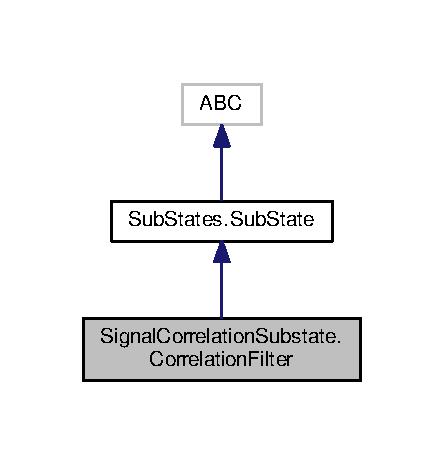
\includegraphics[width=213pt]{classSignalCorrelationSubstate_1_1CorrelationFilter__inherit__graph}
\end{center}
\end{figure}


Collaboration diagram for Signal\+Correlation\+Substate.\+Correlation\+Filter\+:\nopagebreak
\begin{figure}[H]
\begin{center}
\leavevmode
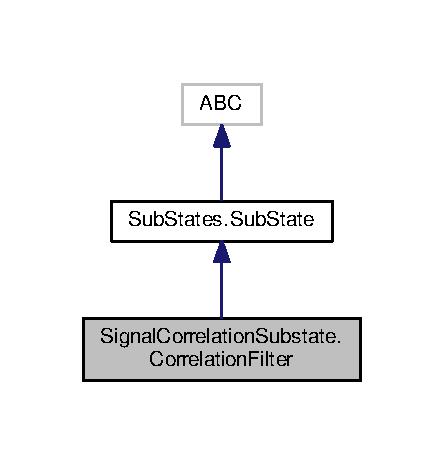
\includegraphics[width=213pt]{classSignalCorrelationSubstate_1_1CorrelationFilter__coll__graph}
\end{center}
\end{figure}
\subsection*{Public Member Functions}
\begin{DoxyCompactItemize}
\item 
def \hyperlink{classSignalCorrelationSubstate_1_1CorrelationFilter_a98d7aaf451122a2bc10fdcffafcf1768}{\+\_\+\+\_\+init\+\_\+\+\_\+} (self, true\+Signal, filter\+Order, dT, \hyperlink{classSignalCorrelationSubstate_1_1CorrelationFilter_a7931bebb63d9482b44f69d31786c4086}{t}=0, \hyperlink{classSignalCorrelationSubstate_1_1CorrelationFilter_ae308a025a3a7ebdf4e66b5fd3fdf2b7d}{correlation\+Vector}=None, \hyperlink{classSignalCorrelationSubstate_1_1CorrelationFilter_a484e6bdabe405d0aba1dcf4d5729dd72}{correlation\+Vector\+Covariance}=None, \hyperlink{classSignalCorrelationSubstate_1_1CorrelationFilter_a01e35890dee1d79bd0e4f9e82cb16e3f}{signal\+Delay}=0, \hyperlink{classSignalCorrelationSubstate_1_1CorrelationFilter_a34d52beb18c131f2305689d48f612a5a}{delay\+Var}=0, \hyperlink{classSignalCorrelationSubstate_1_1CorrelationFilter_a960e7455c5def570629d69a2bf1cb288}{a\+Priori}=True, \hyperlink{classSignalCorrelationSubstate_1_1CorrelationFilter_a8e53182c2ff431a6a545a265cda6ba48}{center\+Peak}=True, \hyperlink{classSignalCorrelationSubstate_1_1CorrelationFilter_a85a73739e9bb0a7f20886a812a3afa83}{peak\+Fit\+Points}=1, \hyperlink{classSignalCorrelationSubstate_1_1CorrelationFilter_abbd9598dd2d237abb1eef86ba427da7f}{process\+Noise}=1e-\/12, measurement\+Noise\+Scale\+Factor=1)
\begin{DoxyCompactList}\small\item\em \hyperlink{classSignalCorrelationSubstate_1_1CorrelationFilter_a98d7aaf451122a2bc10fdcffafcf1768}{\+\_\+\+\_\+init\+\_\+\+\_\+} is responsible for initializing a correlation vector estimator \end{DoxyCompactList}\item 
def \hyperlink{classSignalCorrelationSubstate_1_1CorrelationFilter_ad05512ccd7d825c60f671f8a66306e28}{build\+Time\+Update\+Matrices} (self, deltaT, dynamics, h)
\begin{DoxyCompactList}\small\item\em \hyperlink{classSignalCorrelationSubstate_1_1CorrelationFilter_ad05512ccd7d825c60f671f8a66306e28}{build\+Time\+Update\+Matrices} constructs the correlation vector time update matrices \end{DoxyCompactList}\end{DoxyCompactItemize}
\begin{Indent}{\bf Mandatory Sub\+State Functions}\par
{\em The following functions are required in order for this class to be used as a substate in Modular\+Filter.

The inside of the functions may be changed or updated, but their \char`\"{}black box\char`\"{} behavior must remain the same; i.\+e. they must still perform the same essential functions and return the same things. }\begin{DoxyCompactItemize}
\item 
def \hyperlink{classSignalCorrelationSubstate_1_1CorrelationFilter_a94b5211aa159578344974b52f3b9f92e}{store\+State\+Vector} (self, sv\+Dict)
\begin{DoxyCompactList}\small\item\em \hyperlink{classSignalCorrelationSubstate_1_1CorrelationFilter_a94b5211aa159578344974b52f3b9f92e}{store\+State\+Vector} stores an updated estimate of the state vector \end{DoxyCompactList}\item 
def \hyperlink{classSignalCorrelationSubstate_1_1CorrelationFilter_a07a8c37a30c3d0a057049e0ff2eac67f}{time\+Update} (self, dT, dynamics=None)
\begin{DoxyCompactList}\small\item\em \hyperlink{classSignalCorrelationSubstate_1_1CorrelationFilter_a07a8c37a30c3d0a057049e0ff2eac67f}{time\+Update} returns the matrices for performing the correlation vector time update. \end{DoxyCompactList}\item 
def \hyperlink{classSignalCorrelationSubstate_1_1CorrelationFilter_ae7338456be781e322eba5bce4e41199f}{get\+Measurement\+Matrices} (self, measurement, source=None)
\begin{DoxyCompactList}\small\item\em \hyperlink{classSignalCorrelationSubstate_1_1CorrelationFilter_a94b5211aa159578344974b52f3b9f92e}{store\+State\+Vector} stores an updated estimate of the state vector \end{DoxyCompactList}\end{DoxyCompactItemize}
\end{Indent}
\begin{Indent}{\bf Mandatory Sub\+State Functions}\par
{\em The following functions are functions which are required for the Sub\+State to function as a sub-\/state in \hyperlink{classState_1_1ModularFilter}{State.\+Modular\+Filter}. }\begin{DoxyCompactItemize}
\item 
def \hyperlink{classSubStates_1_1SubState_a3ebd1a120f63ed477ee76999518a8828}{get\+State\+Vector} (self)
\begin{DoxyCompactList}\small\item\em \hyperlink{classSubStates_1_1SubState_a3ebd1a120f63ed477ee76999518a8828}{get\+State\+Vector} returns the most recent value of the state vector \end{DoxyCompactList}\item 
def \hyperlink{classSubStates_1_1SubState_a4d863939fdb98b2739e1e737ec7496ae}{covariance} (self)
\begin{DoxyCompactList}\small\item\em \hyperlink{classSubStates_1_1SubState_a4d863939fdb98b2739e1e737ec7496ae}{covariance} returns the \hyperlink{classSubStates_1_1SubState}{Sub\+State} covariance matrix \end{DoxyCompactList}\item 
def \hyperlink{classSubStates_1_1SubState_a4aebea19a134cb871a7c0b6c2709546a}{dimension} (self)
\begin{DoxyCompactList}\small\item\em \hyperlink{classSubStates_1_1SubState_a4aebea19a134cb871a7c0b6c2709546a}{dimension} returns the dimension of the sub-\/state vector \end{DoxyCompactList}\end{DoxyCompactItemize}
\end{Indent}
\begin{Indent}{\bf Plotting Functions}\par
{\em These functions provide generalized plotting capabilities }\begin{DoxyCompactItemize}
\item 
def \hyperlink{classSubStates_1_1SubState_ab1767fb43256809f722a9f6dc73fef19}{initialize\+Real\+Time\+Plot} (self, plot\+Handle=None, axis\+Handle=None)
\item 
def \hyperlink{classSubStates_1_1SubState_a8df931305220bef14684e76fd6743b0d}{real\+Time\+Plot} (self, normalized=True)
\end{DoxyCompactItemize}
\end{Indent}
\subsection*{Public Attributes}
\begin{DoxyCompactItemize}
\item 
\hyperlink{classSignalCorrelationSubstate_1_1CorrelationFilter_a7931bebb63d9482b44f69d31786c4086}{t}
\begin{DoxyCompactList}\small\item\em \hyperlink{classSignalCorrelationSubstate_1_1CorrelationFilter_a7931bebb63d9482b44f69d31786c4086}{t} The current time \end{DoxyCompactList}\item 
\hyperlink{classSignalCorrelationSubstate_1_1CorrelationFilter_a960e7455c5def570629d69a2bf1cb288}{a\+Priori}
\begin{DoxyCompactList}\small\item\em \hyperlink{classSignalCorrelationSubstate_1_1CorrelationFilter_a960e7455c5def570629d69a2bf1cb288}{a\+Priori} Indicates whether the current state vector is the result of a time update (\hyperlink{classSignalCorrelationSubstate_1_1CorrelationFilter_a960e7455c5def570629d69a2bf1cb288}{a\+Priori} = True) or a measurement update (\hyperlink{classSignalCorrelationSubstate_1_1CorrelationFilter_a960e7455c5def570629d69a2bf1cb288}{a\+Priori} = False) \end{DoxyCompactList}\item 
\hyperlink{classSignalCorrelationSubstate_1_1CorrelationFilter_ae308a025a3a7ebdf4e66b5fd3fdf2b7d}{correlation\+Vector}
\begin{DoxyCompactList}\small\item\em \hyperlink{classSignalCorrelationSubstate_1_1CorrelationFilter_ae308a025a3a7ebdf4e66b5fd3fdf2b7d}{correlation\+Vector} is the current estimate of the correlation vector between the incoming signal measurements and the \hyperlink{classSignalCorrelationSubstate_1_1CorrelationFilter_a5f777d3a877658a1365ebac65b9ab25b}{\+\_\+\+\_\+true\+Signal\+\_\+\+\_\+} \end{DoxyCompactList}\item 
\hyperlink{classSignalCorrelationSubstate_1_1CorrelationFilter_a484e6bdabe405d0aba1dcf4d5729dd72}{correlation\+Vector\+Covariance}
\begin{DoxyCompactList}\small\item\em \hyperlink{classSignalCorrelationSubstate_1_1CorrelationFilter_a484e6bdabe405d0aba1dcf4d5729dd72}{correlation\+Vector\+Covariance} is the covariance matrix of the correlation vector estimate, \hyperlink{classSignalCorrelationSubstate_1_1CorrelationFilter_ae308a025a3a7ebdf4e66b5fd3fdf2b7d}{correlation\+Vector} \end{DoxyCompactList}\item 
\hyperlink{classSignalCorrelationSubstate_1_1CorrelationFilter_a01e35890dee1d79bd0e4f9e82cb16e3f}{signal\+Delay}
\begin{DoxyCompactList}\small\item\em \hyperlink{classSignalCorrelationSubstate_1_1CorrelationFilter_a01e35890dee1d79bd0e4f9e82cb16e3f}{signal\+Delay} is the current estimate of the delay between the incoming signal measurements and the \hyperlink{classSignalCorrelationSubstate_1_1CorrelationFilter_a5f777d3a877658a1365ebac65b9ab25b}{\+\_\+\+\_\+true\+Signal\+\_\+\+\_\+} \end{DoxyCompactList}\item 
\hyperlink{classSignalCorrelationSubstate_1_1CorrelationFilter_a34d52beb18c131f2305689d48f612a5a}{delay\+Var}
\begin{DoxyCompactList}\small\item\em \hyperlink{classSignalCorrelationSubstate_1_1CorrelationFilter_a34d52beb18c131f2305689d48f612a5a}{delay\+Var} is the variance of the signal delay estimate \hyperlink{classSignalCorrelationSubstate_1_1CorrelationFilter_a01e35890dee1d79bd0e4f9e82cb16e3f}{signal\+Delay} \end{DoxyCompactList}\item 
\hyperlink{classSignalCorrelationSubstate_1_1CorrelationFilter_a8e53182c2ff431a6a545a265cda6ba48}{center\+Peak}
\begin{DoxyCompactList}\small\item\em \hyperlink{classSignalCorrelationSubstate_1_1CorrelationFilter_a8e53182c2ff431a6a545a265cda6ba48}{center\+Peak} indicates whether the correlation vector is shifted to maintain the peak at the 0th tap \end{DoxyCompactList}\item 
\hyperlink{classSignalCorrelationSubstate_1_1CorrelationFilter_a85a73739e9bb0a7f20886a812a3afa83}{peak\+Fit\+Points}
\begin{DoxyCompactList}\small\item\em \hyperlink{classSignalCorrelationSubstate_1_1CorrelationFilter_a85a73739e9bb0a7f20886a812a3afa83}{peak\+Fit\+Points} is a variable which controls the number of points used for quadratically estimating the location of the correlation vector peak \end{DoxyCompactList}\item 
\hyperlink{classSignalCorrelationSubstate_1_1CorrelationFilter_abbd9598dd2d237abb1eef86ba427da7f}{process\+Noise}
\begin{DoxyCompactList}\small\item\em \hyperlink{classSignalCorrelationSubstate_1_1CorrelationFilter_abbd9598dd2d237abb1eef86ba427da7f}{process\+Noise} is the scalar value used to generate an additional process noise term in \hyperlink{classSignalCorrelationSubstate_1_1CorrelationFilter_a07a8c37a30c3d0a057049e0ff2eac67f}{time\+Update}. \end{DoxyCompactList}\item 
\hyperlink{classSignalCorrelationSubstate_1_1CorrelationFilter_a21fc425a1d3bcb40b44afbca1f908de1}{measurement\+Noise\+Scale\+Factor}
\begin{DoxyCompactList}\small\item\em \hyperlink{classSignalCorrelationSubstate_1_1CorrelationFilter_a21fc425a1d3bcb40b44afbca1f908de1}{measurement\+Noise\+Scale\+Factor} is a factor used to scale the measurement noise matrix. \end{DoxyCompactList}\item 
\hyperlink{classSubStates_1_1SubState_a24bf2de56fc3037d91cba43d28f3bf60}{state\+Vector\+History}
\begin{DoxyCompactList}\small\item\em Stores the time-\/history of the sub-\/state state vector. \end{DoxyCompactList}\item 
\hyperlink{classSubStates_1_1SubState_ab92a0fafcfd778b8965e3f649ff94fc7}{R\+T\+Plot\+Handle}
\begin{DoxyCompactList}\small\item\em Stores handle for real-\/time plotting. \end{DoxyCompactList}\item 
\hyperlink{classSubStates_1_1SubState_aae3aa07f0d6f54a510db66e0644c958e}{R\+T\+Plot\+Data}
\item 
\hyperlink{classSubStates_1_1SubState_a41c912457be8682326d60f82cc651207}{R\+T\+Paxis\+Handle}
\end{DoxyCompactItemize}
\subsection*{Private Attributes}
\begin{DoxyCompactItemize}
\item 
\hyperlink{classSignalCorrelationSubstate_1_1CorrelationFilter_a18f7cac4d1943bc7f780db22f0355e4a}{\+\_\+\+\_\+unit\+Vec\+To\+Signal\+\_\+\+\_\+}
\begin{DoxyCompactList}\small\item\em \hyperlink{classSignalCorrelationSubstate_1_1CorrelationFilter_a18f7cac4d1943bc7f780db22f0355e4a}{\+\_\+\+\_\+unit\+Vec\+To\+Signal\+\_\+\+\_\+} is a unit vector which points to the signal source \end{DoxyCompactList}\item 
\hyperlink{classSignalCorrelationSubstate_1_1CorrelationFilter_a5f777d3a877658a1365ebac65b9ab25b}{\+\_\+\+\_\+true\+Signal\+\_\+\+\_\+}
\begin{DoxyCompactList}\small\item\em \hyperlink{classSignalCorrelationSubstate_1_1CorrelationFilter_a5f777d3a877658a1365ebac65b9ab25b}{\+\_\+\+\_\+true\+Signal\+\_\+\+\_\+} is a signal object that contains the \char`\"{}true\char`\"{} signal for which the correlation vector is being estimated \end{DoxyCompactList}\item 
\hyperlink{classSignalCorrelationSubstate_1_1CorrelationFilter_a668625040b858deeb1a7e3ad8649abeb}{\+\_\+\+\_\+filter\+Order\+\_\+\+\_\+}
\begin{DoxyCompactList}\small\item\em \hyperlink{classSignalCorrelationSubstate_1_1CorrelationFilter_a668625040b858deeb1a7e3ad8649abeb}{\+\_\+\+\_\+filter\+Order\+\_\+\+\_\+} is the number of \char`\"{}taps\char`\"{} in the estimated correlation vector, \hyperlink{classSignalCorrelationSubstate_1_1CorrelationFilter_ae308a025a3a7ebdf4e66b5fd3fdf2b7d}{correlation\+Vector}. \end{DoxyCompactList}\item 
\hyperlink{classSignalCorrelationSubstate_1_1CorrelationFilter_a0f3b9de9415899aa7d41f0b67216eb99}{\+\_\+\+\_\+d\+T\+\_\+\+\_\+}
\begin{DoxyCompactList}\small\item\em \hyperlink{classSignalCorrelationSubstate_1_1CorrelationFilter_a0f3b9de9415899aa7d41f0b67216eb99}{\+\_\+\+\_\+d\+T\+\_\+\+\_\+} is the \char`\"{}sample period\char`\"{} or \char`\"{}bin size\char`\"{} of the estimated correlation vector \end{DoxyCompactList}\end{DoxyCompactItemize}
\subsection*{Functions Specific to Signal\+Correlation\+Sub\+State.\+Correlation\+Filter}
\label{_amgrpb9fa21aa95ba3ab05a0dfc16edccddcd}%
The following remaining functions are not required in order for this class to be used as a Sub\+State, and may be changed as needed, including inputs and outputs.\begin{DoxyCompactItemize}
\item 
def \hyperlink{classSignalCorrelationSubstate_1_1CorrelationFilter_aa3ce889ae348140fca8acd0fc75ea9a0}{get\+T\+O\+A\+Measurement\+Matrices} (self, measurement, corr\+Vec)
\begin{DoxyCompactList}\small\item\em \hyperlink{classSignalCorrelationSubstate_1_1CorrelationFilter_ace04b6e310f321192715c76ec2ac6b52}{compute\+Signal\+Delay} computes the delay between the \hyperlink{classSignalCorrelationSubstate_1_1CorrelationFilter_a5f777d3a877658a1365ebac65b9ab25b}{\+\_\+\+\_\+true\+Signal\+\_\+\+\_\+} and measurements based on a correlation vector \end{DoxyCompactList}\item 
def \hyperlink{classSignalCorrelationSubstate_1_1CorrelationFilter_ace04b6e310f321192715c76ec2ac6b52}{compute\+Signal\+Delay} (self, c, P)
\begin{DoxyCompactList}\small\item\em \hyperlink{classSignalCorrelationSubstate_1_1CorrelationFilter_ace04b6e310f321192715c76ec2ac6b52}{compute\+Signal\+Delay} computes the delay between the \hyperlink{classSignalCorrelationSubstate_1_1CorrelationFilter_a5f777d3a877658a1365ebac65b9ab25b}{\+\_\+\+\_\+true\+Signal\+\_\+\+\_\+} and measurements based on a correlation vector \end{DoxyCompactList}\item 
def \hyperlink{classSignalCorrelationSubstate_1_1CorrelationFilter_aa9e1991566655a89ed084b6918cfb278}{estimate\+Signal\+Delay\+UT} (self, h, P)
\begin{DoxyCompactList}\small\item\em \hyperlink{classSignalCorrelationSubstate_1_1CorrelationFilter_aa9e1991566655a89ed084b6918cfb278}{estimate\+Signal\+Delay\+UT} uses a unscented tranform to estimate the delay corresponding to a correlation vector \end{DoxyCompactList}\item 
def \hyperlink{classSignalCorrelationSubstate_1_1CorrelationFilter_aae801ac673e939678f865f9c0dc23d55}{speed\+Of\+Light} (self)
\begin{DoxyCompactList}\small\item\em \hyperlink{classSignalCorrelationSubstate_1_1CorrelationFilter_ace04b6e310f321192715c76ec2ac6b52}{compute\+Signal\+Delay} computes the delay between the \hyperlink{classSignalCorrelationSubstate_1_1CorrelationFilter_a5f777d3a877658a1365ebac65b9ab25b}{\+\_\+\+\_\+true\+Signal\+\_\+\+\_\+} and measurements based on a correlation vector \end{DoxyCompactList}\item 
def \hyperlink{classSignalCorrelationSubstate_1_1CorrelationFilter_a948d71970965e18ecc2f19c3bc49f7f7}{sinc\+Diff} (x)
\begin{DoxyCompactList}\small\item\em \hyperlink{classSignalCorrelationSubstate_1_1CorrelationFilter_ace04b6e310f321192715c76ec2ac6b52}{compute\+Signal\+Delay} computes the delay between the \hyperlink{classSignalCorrelationSubstate_1_1CorrelationFilter_a5f777d3a877658a1365ebac65b9ab25b}{\+\_\+\+\_\+true\+Signal\+\_\+\+\_\+} and measurements based on a correlation vector \end{DoxyCompactList}\end{DoxyCompactItemize}


\subsection{Detailed Description}
\hyperlink{classSignalCorrelationSubstate_1_1CorrelationFilter}{Correlation\+Filter} estimates the correlation vector and delay between a signal and a time-\/delayed measurement of that signal. 

This class contains an estimator which estimates the correlation vector between a signal (the \hyperlink{classSignalCorrelationSubstate_1_1CorrelationFilter_a5f777d3a877658a1365ebac65b9ab25b}{\+\_\+\+\_\+true\+Signal\+\_\+\+\_\+}) and measurements of that signal. This correlation vector is then used to estimate the delay between the \hyperlink{classSignalCorrelationSubstate_1_1CorrelationFilter_a5f777d3a877658a1365ebac65b9ab25b}{\+\_\+\+\_\+true\+Signal\+\_\+\+\_\+} and the measurements of that signal.

The estimator in this class currently assumes that the signal source is \char`\"{}distant,\char`\"{} or infinitely far away. This implies that the unit vector to the signal source is perfectly known, and not changing. A later implementation could include the option of having a non-\/distant signal source, in which the unit vector is changing as a function of position and therefore uncertain.

\begin{DoxyNote}{Note}
This class is essentially an implementation of the estimator presented in \href{https://doi.org/10.2514/1.G002650}{\tt Recursive Range Estimation Using Astrophysical Signals of Opportunity}, J. Runnels, D. Gebre, Journal of Guidance, Control and Dynamics, 2017. Some equations from the paper are included in the class documentation for reference. A more detailed discussion and derivation of the estimator can be found in the journal article.. 
\end{DoxyNote}


Definition at line 40 of file Signal\+Correlation\+Substate.\+py.



\subsection{Constructor \& Destructor Documentation}
\index{Signal\+Correlation\+Substate\+::\+Correlation\+Filter@{Signal\+Correlation\+Substate\+::\+Correlation\+Filter}!\+\_\+\+\_\+init\+\_\+\+\_\+@{\+\_\+\+\_\+init\+\_\+\+\_\+}}
\index{\+\_\+\+\_\+init\+\_\+\+\_\+@{\+\_\+\+\_\+init\+\_\+\+\_\+}!Signal\+Correlation\+Substate\+::\+Correlation\+Filter@{Signal\+Correlation\+Substate\+::\+Correlation\+Filter}}
\subsubsection[{\texorpdfstring{\+\_\+\+\_\+init\+\_\+\+\_\+(self, true\+Signal, filter\+Order, d\+T, t=0, correlation\+Vector=\+None, correlation\+Vector\+Covariance=\+None, signal\+Delay=0, delay\+Var=0, a\+Priori=\+True, center\+Peak=\+True, peak\+Fit\+Points=1, process\+Noise=1e-\/12, measurement\+Noise\+Scale\+Factor=1)}{__init__(self, trueSignal, filterOrder, dT, t=0, correlationVector=None, correlationVectorCovariance=None, signalDelay=0, delayVar=0, aPriori=True, centerPeak=True, peakFitPoints=1, processNoise=1e-12, measurementNoiseScaleFactor=1)}}]{\setlength{\rightskip}{0pt plus 5cm}def Signal\+Correlation\+Substate.\+Correlation\+Filter.\+\_\+\+\_\+init\+\_\+\+\_\+ (
\begin{DoxyParamCaption}
\item[{}]{self, }
\item[{}]{true\+Signal, }
\item[{}]{filter\+Order, }
\item[{}]{dT, }
\item[{}]{t = {\ttfamily 0}, }
\item[{}]{correlation\+Vector = {\ttfamily None}, }
\item[{}]{correlation\+Vector\+Covariance = {\ttfamily None}, }
\item[{}]{signal\+Delay = {\ttfamily 0}, }
\item[{}]{delay\+Var = {\ttfamily 0}, }
\item[{}]{a\+Priori = {\ttfamily True}, }
\item[{}]{center\+Peak = {\ttfamily True}, }
\item[{}]{peak\+Fit\+Points = {\ttfamily 1}, }
\item[{}]{process\+Noise = {\ttfamily 1e-\/12}, }
\item[{}]{measurement\+Noise\+Scale\+Factor = {\ttfamily 1}}
\end{DoxyParamCaption}
)}\hypertarget{classSignalCorrelationSubstate_1_1CorrelationFilter_a98d7aaf451122a2bc10fdcffafcf1768}{}\label{classSignalCorrelationSubstate_1_1CorrelationFilter_a98d7aaf451122a2bc10fdcffafcf1768}


\hyperlink{classSignalCorrelationSubstate_1_1CorrelationFilter_a98d7aaf451122a2bc10fdcffafcf1768}{\+\_\+\+\_\+init\+\_\+\+\_\+} is responsible for initializing a correlation vector estimator 

The primary function of the \hyperlink{classSignalCorrelationSubstate_1_1CorrelationFilter_a98d7aaf451122a2bc10fdcffafcf1768}{\+\_\+\+\_\+init\+\_\+\+\_\+} method is to initialize the correlation vector estimator, and store the relevant user inputs. A few key user inputs are required in order to initialize the filter. Additionally, because the algorithm is relatively complicated, there are a number of optional tuning parameters which may be inputed at initialization.

In general, the parameters which are required inputs are the ones that are critical for initialization of the filter, and should not be changed during the course of the filter\textquotesingle{}s lifetime. These inputs are stored as \char`\"{}private\char`\"{} variables; indicating that the should not be changed during the object\textquotesingle{}s lifetime.

The optional inputs, on the other hand, are inputs which are used in the estimation functions (\hyperlink{classSignalCorrelationSubstate_1_1CorrelationFilter_a07a8c37a30c3d0a057049e0ff2eac67f}{time\+Update}, \hyperlink{classSignalCorrelationSubstate_1_1CorrelationFilter_ae7338456be781e322eba5bce4e41199f}{get\+Measurement\+Matrices}, etc.). These parameters could conceivably be changed during the lifetime of the filter without causing problems, and the user may want to change them depending on external factors. These parameters are initalized with default values, and stored as public variables that the user can in theory change.

There are also a set of class variables which are publicly accessable and which hold the most recent state estimate. These exist primarily for convenience, and are never actually used within the class. Modifying them will have no affect on the state estimates. The only way to modify a state estimate is through the \hyperlink{classSignalCorrelationSubstate_1_1CorrelationFilter_a94b5211aa159578344974b52f3b9f92e}{store\+State\+Vector} method.

The \hyperlink{classSignalCorrelationSubstate_1_1CorrelationFilter_a98d7aaf451122a2bc10fdcffafcf1768}{\+\_\+\+\_\+init\+\_\+\+\_\+} method also checks the user inputs to ensure that they are consistent with how they will be used in the class (where applicable).

The true\+Signal input is checked to see whether it has the following methods\+:
\begin{DoxyItemize}
\item flux()
\item peak\+Amplitude()
\item signal\+I\+D()
\item unit\+Vec()
\end{DoxyItemize}


\begin{DoxyParams}[1]{Parameters}
 & {\em true\+Signal} & An object that describes the signal for which correlation should be estimated. \\
\hline
 & {\em filter\+Order} & The number of bins or \char`\"{}taps\char`\"{} in the correlation vector \\
\hline
 & {\em dT} & The sampling period, or time-\/step between bins in the correlation vector\\
\hline
 & {\em t} & (optional) The initial starting time. If no value is passed, initialized to zero by default. \\
\hline
 & {\em correlation\+Vector} & (optional) The initial value of the correlation vector. If not supplied, the correlation vector will be initialized based on the filter \hyperlink{classSignalCorrelationSubstate_1_1CorrelationFilter_a0f3b9de9415899aa7d41f0b67216eb99}{\+\_\+\+\_\+d\+T\+\_\+\+\_\+} and maximum flux of the \hyperlink{classSignalCorrelationSubstate_1_1CorrelationFilter_a5f777d3a877658a1365ebac65b9ab25b}{\+\_\+\+\_\+true\+Signal\+\_\+\+\_\+}. \\
\hline
 & {\em correlation\+Vector\+Covariance} & (optional) The initial value of the correlation vector estimate covariance. If not supplied, the covariance matrix will be initialized based on the filter \hyperlink{classSignalCorrelationSubstate_1_1CorrelationFilter_a0f3b9de9415899aa7d41f0b67216eb99}{\+\_\+\+\_\+d\+T\+\_\+\+\_\+} and maximum flux of \hyperlink{classSignalCorrelationSubstate_1_1CorrelationFilter_a5f777d3a877658a1365ebac65b9ab25b}{\+\_\+\+\_\+true\+Signal\+\_\+\+\_\+}. \\
\hline
 & {\em signal\+Delay} & (optional) The initial estimate of delay between the \hyperlink{classSignalCorrelationSubstate_1_1CorrelationFilter_a5f777d3a877658a1365ebac65b9ab25b}{\+\_\+\+\_\+true\+Signal\+\_\+\+\_\+} and the signal measurements. If not supplied, \hyperlink{classSignalCorrelationSubstate_1_1CorrelationFilter_a01e35890dee1d79bd0e4f9e82cb16e3f}{signal\+Delay} is initialized to zero. \\
\hline
 & {\em delay\+Var} & (optional) The variance of the estimate of delay \\
\hline
 & {\em a\+Priori} & (optional) Indicates whether initial estimates are a priori or a posteriori. Default=True\\
\hline
 & {\em center\+Peak} & (optional) Boolean indicating whether the correlation vector should be \char`\"{}shifted\char`\"{} after each update to keep the peak centered at the zero index. Default is True. \\
\hline
 & {\em peak\+Fit\+Points} & (optional) Number of points used on either side of max for quadratic fit in \hyperlink{classSignalCorrelationSubstate_1_1CorrelationFilter_ace04b6e310f321192715c76ec2ac6b52}{compute\+Signal\+Delay}. Minimum is 1, default is 1. \\
\hline
 & {\em process\+Noise} & (optional) Scalar term of additional process noise added to covariance matrix in time update. Default is 1e-\/12 \\
\hline
 & {\em measurement\+Noise\+Scale\+Factor} & (optional) Scale factor to inflate the measurement noise. Default is 1. \\
\hline
\end{DoxyParams}


Definition at line 129 of file Signal\+Correlation\+Substate.\+py.



\subsection{Member Function Documentation}
\index{Signal\+Correlation\+Substate\+::\+Correlation\+Filter@{Signal\+Correlation\+Substate\+::\+Correlation\+Filter}!build\+Time\+Update\+Matrices@{build\+Time\+Update\+Matrices}}
\index{build\+Time\+Update\+Matrices@{build\+Time\+Update\+Matrices}!Signal\+Correlation\+Substate\+::\+Correlation\+Filter@{Signal\+Correlation\+Substate\+::\+Correlation\+Filter}}
\subsubsection[{\texorpdfstring{build\+Time\+Update\+Matrices(self, delta\+T, dynamics, h)}{buildTimeUpdateMatrices(self, deltaT, dynamics, h)}}]{\setlength{\rightskip}{0pt plus 5cm}def Signal\+Correlation\+Substate.\+Correlation\+Filter.\+build\+Time\+Update\+Matrices (
\begin{DoxyParamCaption}
\item[{}]{self, }
\item[{}]{deltaT, }
\item[{}]{dynamics, }
\item[{}]{h}
\end{DoxyParamCaption}
)}\hypertarget{classSignalCorrelationSubstate_1_1CorrelationFilter_ad05512ccd7d825c60f671f8a66306e28}{}\label{classSignalCorrelationSubstate_1_1CorrelationFilter_ad05512ccd7d825c60f671f8a66306e28}


\hyperlink{classSignalCorrelationSubstate_1_1CorrelationFilter_ad05512ccd7d825c60f671f8a66306e28}{build\+Time\+Update\+Matrices} constructs the correlation vector time update matrices 

The \hyperlink{classSignalCorrelationSubstate_1_1CorrelationFilter_ad05512ccd7d825c60f671f8a66306e28}{build\+Time\+Update\+Matrices} method constructs the matrices required to perform the time update of the correlation vector sub-\/state.

The time update matrices are a function of the estimated spacecraft velocity ( $\mathbf{v}$), velocity variance ( $\mathbf{P}_{\mathbf{v}}$), and the elapsed time over which the time update occurs ( $\Delta T$). The matrices are constructed as follows\+:

\[ \mathbf{F}_{j \to k} = \begin{bmatrix} \textrm{sinc}(\hat{\delta}) & \hdots & \textrm{sinc}(\hat{\delta} + N - 1) \\ \vdots & \ddots & \vdots \\ \textrm{sinc}(\hat{\delta} - N + 1) & \hdots & \textrm{sinc}(\hat{\delta}) \end{bmatrix} \]

\[ \mathbf{L}_{j} = \begin{bmatrix} \frac{\textrm{cos}}{(\hat{\delta})} - \frac{\textrm{sin}}{(\hat{\delta}^2)} & \hdots \\ \vdots & \ddots \\ \end{bmatrix} \sv[timeIndex = k] \]

\[ Q_{\delta} = \left(\frac{(k-j)}{c}\right)^2 {\LOSVec[S]}^T \mathbf{P}_{\mathbf{v}} \LOSVec[S] \]

where

\[ \hat{\delta}_{j \to k} = \frac{\mathbf{v} \LOSVec[S] \Delta T}{c T} \]


\begin{DoxyParams}{Parameters}
{\em self} & The object pointer \\
\hline
{\em deltaT} & The amount of time over which the time update is occuring \\
\hline
{\em dynamics} & A dictionary containing the relevant dynamics for the time update \\
\hline
{\em h} & The current correlation vector\\
\hline
\end{DoxyParams}
\begin{DoxyReturn}{Returns}
A dictionary containing the matrices $\mathbf{F}$, $\mathbf{L}$, and the scalar 
\end{DoxyReturn}


Definition at line 357 of file Signal\+Correlation\+Substate.\+py.

\index{Signal\+Correlation\+Substate\+::\+Correlation\+Filter@{Signal\+Correlation\+Substate\+::\+Correlation\+Filter}!compute\+Signal\+Delay@{compute\+Signal\+Delay}}
\index{compute\+Signal\+Delay@{compute\+Signal\+Delay}!Signal\+Correlation\+Substate\+::\+Correlation\+Filter@{Signal\+Correlation\+Substate\+::\+Correlation\+Filter}}
\subsubsection[{\texorpdfstring{compute\+Signal\+Delay(self, c, P)}{computeSignalDelay(self, c, P)}}]{\setlength{\rightskip}{0pt plus 5cm}def Signal\+Correlation\+Substate.\+Correlation\+Filter.\+compute\+Signal\+Delay (
\begin{DoxyParamCaption}
\item[{}]{self, }
\item[{}]{c, }
\item[{}]{P}
\end{DoxyParamCaption}
)}\hypertarget{classSignalCorrelationSubstate_1_1CorrelationFilter_ace04b6e310f321192715c76ec2ac6b52}{}\label{classSignalCorrelationSubstate_1_1CorrelationFilter_ace04b6e310f321192715c76ec2ac6b52}


\hyperlink{classSignalCorrelationSubstate_1_1CorrelationFilter_ace04b6e310f321192715c76ec2ac6b52}{compute\+Signal\+Delay} computes the delay between the \hyperlink{classSignalCorrelationSubstate_1_1CorrelationFilter_a5f777d3a877658a1365ebac65b9ab25b}{\+\_\+\+\_\+true\+Signal\+\_\+\+\_\+} and measurements based on a correlation vector 

The \hyperlink{classSignalCorrelationSubstate_1_1CorrelationFilter_ace04b6e310f321192715c76ec2ac6b52}{compute\+Signal\+Delay} function is a rudimentary function which takes an estimate of the correlation vector and uses it to estimate the location of the peak. It functions by finding the tap with the maximum value, and then fitting a quadratic to the points surrounding the maximum value tap. The number of points to which the quadratic is fitted is determined by the value of \hyperlink{classSignalCorrelationSubstate_1_1CorrelationFilter_a85a73739e9bb0a7f20886a812a3afa83}{peak\+Fit\+Points}; the number of points is equal to $2 * n + 1$ where $n = $ \hyperlink{classSignalCorrelationSubstate_1_1CorrelationFilter_a85a73739e9bb0a7f20886a812a3afa83}{peak\+Fit\+Points}.

The delay estimate that is returned is in units of \hyperlink{classSignalCorrelationSubstate_1_1CorrelationFilter_a0f3b9de9415899aa7d41f0b67216eb99}{\+\_\+\+\_\+d\+T\+\_\+\+\_\+}. So, a returned value of 2 would imply that the peak is located at 2, and therefore the delay corresponding to the correlation vector is 2 \hyperlink{classSignalCorrelationSubstate_1_1CorrelationFilter_a0f3b9de9415899aa7d41f0b67216eb99}{\+\_\+\+\_\+d\+T\+\_\+\+\_\+}.

The returned delay may not include previously accumulated \hyperlink{classSignalCorrelationSubstate_1_1CorrelationFilter_a01e35890dee1d79bd0e4f9e82cb16e3f}{signal\+Delay} between the signal and the measurements. See the \hyperlink{classSignalCorrelationSubstate_1_1CorrelationFilter_a94b5211aa159578344974b52f3b9f92e}{store\+State\+Vector} function for more information on how the \hyperlink{classSignalCorrelationSubstate_1_1CorrelationFilter_a01e35890dee1d79bd0e4f9e82cb16e3f}{signal\+Delay} is stored and accumulated delay is accounted for.


\begin{DoxyParams}{Parameters}
{\em self} & The object pointer \\
\hline
{\em c} & The correlation vector \\
\hline
{\em P} & the correlation vector covariance matrix\\
\hline
\end{DoxyParams}
\begin{DoxyReturn}{Returns}
The estimate of the delay 
\end{DoxyReturn}


Definition at line 513 of file Signal\+Correlation\+Substate.\+py.

\index{Signal\+Correlation\+Substate\+::\+Correlation\+Filter@{Signal\+Correlation\+Substate\+::\+Correlation\+Filter}!covariance@{covariance}}
\index{covariance@{covariance}!Signal\+Correlation\+Substate\+::\+Correlation\+Filter@{Signal\+Correlation\+Substate\+::\+Correlation\+Filter}}
\subsubsection[{\texorpdfstring{covariance(self)}{covariance(self)}}]{\setlength{\rightskip}{0pt plus 5cm}def Sub\+States.\+Sub\+State.\+covariance (
\begin{DoxyParamCaption}
\item[{}]{self}
\end{DoxyParamCaption}
)\hspace{0.3cm}{\ttfamily [inherited]}}\hypertarget{classSubStates_1_1SubState_a4d863939fdb98b2739e1e737ec7496ae}{}\label{classSubStates_1_1SubState_a4d863939fdb98b2739e1e737ec7496ae}


\hyperlink{classSubStates_1_1SubState_a4d863939fdb98b2739e1e737ec7496ae}{covariance} returns the \hyperlink{classSubStates_1_1SubState}{Sub\+State} covariance matrix 

The \hyperlink{classSubStates_1_1SubState_a4d863939fdb98b2739e1e737ec7496ae}{covariance} method returns the covariance of the estimate of the substate.

\begin{DoxyRefDesc}{Todo}
\item[\hyperlink{todo__todo000001}{Todo}]Currently, this method only returns the covariance of the most recent state estimate. Ideally, there should be an optional time parameter which would allow the user to get the covaraince matrix at a specified time (or the closest to that specified time).\end{DoxyRefDesc}



\begin{DoxyParams}{Parameters}
{\em self} & The object pointer\\
\hline
\end{DoxyParams}
\begin{DoxyReturn}{Returns}
Returns the covaraince matrix 
\end{DoxyReturn}


Definition at line 172 of file Sub\+States.\+py.

\index{Signal\+Correlation\+Substate\+::\+Correlation\+Filter@{Signal\+Correlation\+Substate\+::\+Correlation\+Filter}!dimension@{dimension}}
\index{dimension@{dimension}!Signal\+Correlation\+Substate\+::\+Correlation\+Filter@{Signal\+Correlation\+Substate\+::\+Correlation\+Filter}}
\subsubsection[{\texorpdfstring{dimension(self)}{dimension(self)}}]{\setlength{\rightskip}{0pt plus 5cm}def Sub\+States.\+Sub\+State.\+dimension (
\begin{DoxyParamCaption}
\item[{}]{self}
\end{DoxyParamCaption}
)\hspace{0.3cm}{\ttfamily [inherited]}}\hypertarget{classSubStates_1_1SubState_a4aebea19a134cb871a7c0b6c2709546a}{}\label{classSubStates_1_1SubState_a4aebea19a134cb871a7c0b6c2709546a}


\hyperlink{classSubStates_1_1SubState_a4aebea19a134cb871a7c0b6c2709546a}{dimension} returns the dimension of the sub-\/state vector 

The \hyperlink{classSubStates_1_1SubState_a4aebea19a134cb871a7c0b6c2709546a}{dimension} method returns the dimension of the sub-\/state vector estimated by the \hyperlink{classSubStates_1_1SubState}{Sub\+State}. This is the dimension as seen by the Modular\+Filter estimator.

The default implementation is to return the class variable \hyperlink{classSubStates_1_1SubState_aea750997b2a75daee4a3147eac68e4f8}{\+\_\+\+\_\+dimension\+\_\+\+\_\+}, which is saved at initialization. This is designated as a \char`\"{}protected\char`\"{} variable, and should not change during the course of the \hyperlink{classSubStates_1_1SubState}{Sub\+State}\textquotesingle{}s lifetime. If child class overwrites this implementation, care should be taken to ensure that the value returned by \hyperlink{classSubStates_1_1SubState_a4aebea19a134cb871a7c0b6c2709546a}{dimension} does not change over \hyperlink{classSubStates_1_1SubState}{Sub\+State} object lifetime.

For \hyperlink{classSubStates_1_1SubState}{Sub\+State} objects with auxilary states, or other quantities related to the state vector but not directly estimated by the Modular\+Filter, \hyperlink{classSubStates_1_1SubState_a4aebea19a134cb871a7c0b6c2709546a}{dimension} should not count these states as part of the total dimension.


\begin{DoxyParams}{Parameters}
{\em self} & The object pointer\\
\hline
\end{DoxyParams}
\begin{DoxyReturn}{Returns}
Returns the dimension of state vector 
\end{DoxyReturn}


Definition at line 197 of file Sub\+States.\+py.

\index{Signal\+Correlation\+Substate\+::\+Correlation\+Filter@{Signal\+Correlation\+Substate\+::\+Correlation\+Filter}!estimate\+Signal\+Delay\+UT@{estimate\+Signal\+Delay\+UT}}
\index{estimate\+Signal\+Delay\+UT@{estimate\+Signal\+Delay\+UT}!Signal\+Correlation\+Substate\+::\+Correlation\+Filter@{Signal\+Correlation\+Substate\+::\+Correlation\+Filter}}
\subsubsection[{\texorpdfstring{estimate\+Signal\+Delay\+U\+T(self, h, P)}{estimateSignalDelayUT(self, h, P)}}]{\setlength{\rightskip}{0pt plus 5cm}def Signal\+Correlation\+Substate.\+Correlation\+Filter.\+estimate\+Signal\+Delay\+UT (
\begin{DoxyParamCaption}
\item[{}]{self, }
\item[{}]{h, }
\item[{}]{P}
\end{DoxyParamCaption}
)}\hypertarget{classSignalCorrelationSubstate_1_1CorrelationFilter_aa9e1991566655a89ed084b6918cfb278}{}\label{classSignalCorrelationSubstate_1_1CorrelationFilter_aa9e1991566655a89ed084b6918cfb278}


\hyperlink{classSignalCorrelationSubstate_1_1CorrelationFilter_aa9e1991566655a89ed084b6918cfb278}{estimate\+Signal\+Delay\+UT} uses a unscented tranform to estimate the delay corresponding to a correlation vector 

The \hyperlink{classSignalCorrelationSubstate_1_1CorrelationFilter_aa9e1991566655a89ed084b6918cfb278}{estimate\+Signal\+Delay\+UT} method is responsible for computing the estimated value of delay corresponding to a correlation vector, as well as the variance of that estimate. These values are computed using a unscented transform (i.\+e. sigma-\/point) approach.

The method receives the an estimate of the correlation vector, as well as the covariance matrix corresponding to that vector. From there it computes a set of n sigma points (where n is the length of the correlation vector), and for each of the generated sigma point vectors, it computes the peak location using the \hyperlink{classSignalCorrelationSubstate_1_1CorrelationFilter_ace04b6e310f321192715c76ec2ac6b52}{compute\+Signal\+Delay} method.


\begin{DoxyParams}{Parameters}
{\em self} & The object pointer \\
\hline
{\em h} & The correlation vector \\
\hline
{\em P} & The correlation vector covariance matrix\\
\hline
\end{DoxyParams}
\begin{DoxyReturn}{Returns}
A dict containing the estimate of the peak location (\char`\"{}mean\+Delay\char`\"{}) and the estimate variance (\char`\"{}var\+Delay\char`\"{}) 
\end{DoxyReturn}


Definition at line 588 of file Signal\+Correlation\+Substate.\+py.

\index{Signal\+Correlation\+Substate\+::\+Correlation\+Filter@{Signal\+Correlation\+Substate\+::\+Correlation\+Filter}!get\+Measurement\+Matrices@{get\+Measurement\+Matrices}}
\index{get\+Measurement\+Matrices@{get\+Measurement\+Matrices}!Signal\+Correlation\+Substate\+::\+Correlation\+Filter@{Signal\+Correlation\+Substate\+::\+Correlation\+Filter}}
\subsubsection[{\texorpdfstring{get\+Measurement\+Matrices(self, measurement, source=\+None)}{getMeasurementMatrices(self, measurement, source=None)}}]{\setlength{\rightskip}{0pt plus 5cm}def Signal\+Correlation\+Substate.\+Correlation\+Filter.\+get\+Measurement\+Matrices (
\begin{DoxyParamCaption}
\item[{}]{self, }
\item[{}]{measurement, }
\item[{}]{source = {\ttfamily None}}
\end{DoxyParamCaption}
)}\hypertarget{classSignalCorrelationSubstate_1_1CorrelationFilter_ae7338456be781e322eba5bce4e41199f}{}\label{classSignalCorrelationSubstate_1_1CorrelationFilter_ae7338456be781e322eba5bce4e41199f}


\hyperlink{classSignalCorrelationSubstate_1_1CorrelationFilter_a94b5211aa159578344974b52f3b9f92e}{store\+State\+Vector} stores an updated estimate of the state vector 



Definition at line 285 of file Signal\+Correlation\+Substate.\+py.

\index{Signal\+Correlation\+Substate\+::\+Correlation\+Filter@{Signal\+Correlation\+Substate\+::\+Correlation\+Filter}!get\+State\+Vector@{get\+State\+Vector}}
\index{get\+State\+Vector@{get\+State\+Vector}!Signal\+Correlation\+Substate\+::\+Correlation\+Filter@{Signal\+Correlation\+Substate\+::\+Correlation\+Filter}}
\subsubsection[{\texorpdfstring{get\+State\+Vector(self)}{getStateVector(self)}}]{\setlength{\rightskip}{0pt plus 5cm}def Sub\+States.\+Sub\+State.\+get\+State\+Vector (
\begin{DoxyParamCaption}
\item[{}]{self}
\end{DoxyParamCaption}
)\hspace{0.3cm}{\ttfamily [inherited]}}\hypertarget{classSubStates_1_1SubState_a3ebd1a120f63ed477ee76999518a8828}{}\label{classSubStates_1_1SubState_a3ebd1a120f63ed477ee76999518a8828}


\hyperlink{classSubStates_1_1SubState_a3ebd1a120f63ed477ee76999518a8828}{get\+State\+Vector} returns the most recent value of the state vector 

The \hyperlink{classSubStates_1_1SubState_a3ebd1a120f63ed477ee76999518a8828}{get\+State\+Vector} method is responsible for returning a dictionary object containing, at minimim, the following items\+:


\begin{DoxyItemize}
\item \textquotesingle{}state\+Vector\textquotesingle{}\+: A length \hyperlink{classSubStates_1_1SubState_a4aebea19a134cb871a7c0b6c2709546a}{dimension} array containing the most recent state vector estimate
\item \textquotesingle{}covariance\textquotesingle{}\+: A (\hyperlink{classSubStates_1_1SubState_a4aebea19a134cb871a7c0b6c2709546a}{dimension} x \hyperlink{classSubStates_1_1SubState_a4aebea19a134cb871a7c0b6c2709546a}{dimension}) array containing the most recent covariance matrix
\item \textquotesingle{}a\+Priori\textquotesingle{}\+: A boolean indicating if the most recent estimate is the
\item result of a time update (a\+Priori=True) or a measurement update (a\+Priori=False)
\end{DoxyItemize}

This function can be used as-\/is


\begin{DoxyParams}{Parameters}
{\em self} & The object pointer\\
\hline
\end{DoxyParams}
\begin{DoxyReturn}{Returns}
The dictionary containing the state vector, covariance matrix, and a\+Priori status 
\end{DoxyReturn}


Definition at line 129 of file Sub\+States.\+py.

\index{Signal\+Correlation\+Substate\+::\+Correlation\+Filter@{Signal\+Correlation\+Substate\+::\+Correlation\+Filter}!get\+T\+O\+A\+Measurement\+Matrices@{get\+T\+O\+A\+Measurement\+Matrices}}
\index{get\+T\+O\+A\+Measurement\+Matrices@{get\+T\+O\+A\+Measurement\+Matrices}!Signal\+Correlation\+Substate\+::\+Correlation\+Filter@{Signal\+Correlation\+Substate\+::\+Correlation\+Filter}}
\subsubsection[{\texorpdfstring{get\+T\+O\+A\+Measurement\+Matrices(self, measurement, corr\+Vec)}{getTOAMeasurementMatrices(self, measurement, corrVec)}}]{\setlength{\rightskip}{0pt plus 5cm}def Signal\+Correlation\+Substate.\+Correlation\+Filter.\+get\+T\+O\+A\+Measurement\+Matrices (
\begin{DoxyParamCaption}
\item[{}]{self, }
\item[{}]{measurement, }
\item[{}]{corr\+Vec}
\end{DoxyParamCaption}
)}\hypertarget{classSignalCorrelationSubstate_1_1CorrelationFilter_aa3ce889ae348140fca8acd0fc75ea9a0}{}\label{classSignalCorrelationSubstate_1_1CorrelationFilter_aa3ce889ae348140fca8acd0fc75ea9a0}


\hyperlink{classSignalCorrelationSubstate_1_1CorrelationFilter_ace04b6e310f321192715c76ec2ac6b52}{compute\+Signal\+Delay} computes the delay between the \hyperlink{classSignalCorrelationSubstate_1_1CorrelationFilter_a5f777d3a877658a1365ebac65b9ab25b}{\+\_\+\+\_\+true\+Signal\+\_\+\+\_\+} and measurements based on a correlation vector 

The \hyperlink{classSignalCorrelationSubstate_1_1CorrelationFilter_ace04b6e310f321192715c76ec2ac6b52}{compute\+Signal\+Delay} function is a rudimentary function which takes an estimate of the correlation vector and uses it to estimate the location of the peak. It functions by finding the tap with the maximum value, and then fitting a quadratic to the points surrounding the maximum value tap. The number of points to which the quadratic is fitted is determined by the value of \hyperlink{classSignalCorrelationSubstate_1_1CorrelationFilter_a85a73739e9bb0a7f20886a812a3afa83}{peak\+Fit\+Points}; the number of points is equal to $2 * n + 1$ where $n = $ \hyperlink{classSignalCorrelationSubstate_1_1CorrelationFilter_a85a73739e9bb0a7f20886a812a3afa83}{peak\+Fit\+Points}.

The delay estimate that is returned is in units of \hyperlink{classSignalCorrelationSubstate_1_1CorrelationFilter_a0f3b9de9415899aa7d41f0b67216eb99}{\+\_\+\+\_\+d\+T\+\_\+\+\_\+}. So, a returned value of 2 would imply that the peak is located at 2, and therefore the delay corresponding to the correlation vector is 2 \hyperlink{classSignalCorrelationSubstate_1_1CorrelationFilter_a0f3b9de9415899aa7d41f0b67216eb99}{\+\_\+\+\_\+d\+T\+\_\+\+\_\+}.

The returned delay may not include previously accumulated \hyperlink{classSignalCorrelationSubstate_1_1CorrelationFilter_a01e35890dee1d79bd0e4f9e82cb16e3f}{signal\+Delay} between the signal and the measurements. See the \hyperlink{classSignalCorrelationSubstate_1_1CorrelationFilter_a94b5211aa159578344974b52f3b9f92e}{store\+State\+Vector} function for more information on how the \hyperlink{classSignalCorrelationSubstate_1_1CorrelationFilter_a01e35890dee1d79bd0e4f9e82cb16e3f}{signal\+Delay} is stored and accumulated delay is accounted for.


\begin{DoxyParams}{Parameters}
{\em self} & The object pointer \\
\hline
{\em c} & The correlation vector \\
\hline
{\em P} & the correlation vector covariance matrix\\
\hline
\end{DoxyParams}
\begin{DoxyReturn}{Returns}
The estimate of the delay 
\end{DoxyReturn}


Definition at line 445 of file Signal\+Correlation\+Substate.\+py.

\index{Signal\+Correlation\+Substate\+::\+Correlation\+Filter@{Signal\+Correlation\+Substate\+::\+Correlation\+Filter}!initialize\+Real\+Time\+Plot@{initialize\+Real\+Time\+Plot}}
\index{initialize\+Real\+Time\+Plot@{initialize\+Real\+Time\+Plot}!Signal\+Correlation\+Substate\+::\+Correlation\+Filter@{Signal\+Correlation\+Substate\+::\+Correlation\+Filter}}
\subsubsection[{\texorpdfstring{initialize\+Real\+Time\+Plot(self, plot\+Handle=\+None, axis\+Handle=\+None)}{initializeRealTimePlot(self, plotHandle=None, axisHandle=None)}}]{\setlength{\rightskip}{0pt plus 5cm}def Sub\+States.\+Sub\+State.\+initialize\+Real\+Time\+Plot (
\begin{DoxyParamCaption}
\item[{}]{self, }
\item[{}]{plot\+Handle = {\ttfamily None}, }
\item[{}]{axis\+Handle = {\ttfamily None}}
\end{DoxyParamCaption}
)\hspace{0.3cm}{\ttfamily [inherited]}}\hypertarget{classSubStates_1_1SubState_ab1767fb43256809f722a9f6dc73fef19}{}\label{classSubStates_1_1SubState_ab1767fb43256809f722a9f6dc73fef19}


Definition at line 257 of file Sub\+States.\+py.

\index{Signal\+Correlation\+Substate\+::\+Correlation\+Filter@{Signal\+Correlation\+Substate\+::\+Correlation\+Filter}!real\+Time\+Plot@{real\+Time\+Plot}}
\index{real\+Time\+Plot@{real\+Time\+Plot}!Signal\+Correlation\+Substate\+::\+Correlation\+Filter@{Signal\+Correlation\+Substate\+::\+Correlation\+Filter}}
\subsubsection[{\texorpdfstring{real\+Time\+Plot(self, normalized=\+True)}{realTimePlot(self, normalized=True)}}]{\setlength{\rightskip}{0pt plus 5cm}def Sub\+States.\+Sub\+State.\+real\+Time\+Plot (
\begin{DoxyParamCaption}
\item[{}]{self, }
\item[{}]{normalized = {\ttfamily True}}
\end{DoxyParamCaption}
)\hspace{0.3cm}{\ttfamily [inherited]}}\hypertarget{classSubStates_1_1SubState_a8df931305220bef14684e76fd6743b0d}{}\label{classSubStates_1_1SubState_a8df931305220bef14684e76fd6743b0d}


Definition at line 283 of file Sub\+States.\+py.

\index{Signal\+Correlation\+Substate\+::\+Correlation\+Filter@{Signal\+Correlation\+Substate\+::\+Correlation\+Filter}!sinc\+Diff@{sinc\+Diff}}
\index{sinc\+Diff@{sinc\+Diff}!Signal\+Correlation\+Substate\+::\+Correlation\+Filter@{Signal\+Correlation\+Substate\+::\+Correlation\+Filter}}
\subsubsection[{\texorpdfstring{sinc\+Diff(x)}{sincDiff(x)}}]{\setlength{\rightskip}{0pt plus 5cm}def Signal\+Correlation\+Substate.\+Correlation\+Filter.\+sinc\+Diff (
\begin{DoxyParamCaption}
\item[{}]{x}
\end{DoxyParamCaption}
)\hspace{0.3cm}{\ttfamily [static]}}\hypertarget{classSignalCorrelationSubstate_1_1CorrelationFilter_a948d71970965e18ecc2f19c3bc49f7f7}{}\label{classSignalCorrelationSubstate_1_1CorrelationFilter_a948d71970965e18ecc2f19c3bc49f7f7}


\hyperlink{classSignalCorrelationSubstate_1_1CorrelationFilter_ace04b6e310f321192715c76ec2ac6b52}{compute\+Signal\+Delay} computes the delay between the \hyperlink{classSignalCorrelationSubstate_1_1CorrelationFilter_a5f777d3a877658a1365ebac65b9ab25b}{\+\_\+\+\_\+true\+Signal\+\_\+\+\_\+} and measurements based on a correlation vector 

The \hyperlink{classSignalCorrelationSubstate_1_1CorrelationFilter_ace04b6e310f321192715c76ec2ac6b52}{compute\+Signal\+Delay} function is a rudimentary function which takes an estimate of the correlation vector and uses it to estimate the location of the peak. It functions by finding the tap with the maximum value, and then fitting a quadratic to the points surrounding the maximum value tap. The number of points to which the quadratic is fitted is determined by the value of \hyperlink{classSignalCorrelationSubstate_1_1CorrelationFilter_a85a73739e9bb0a7f20886a812a3afa83}{peak\+Fit\+Points}; the number of points is equal to $2 * n + 1$ where $n = $ \hyperlink{classSignalCorrelationSubstate_1_1CorrelationFilter_a85a73739e9bb0a7f20886a812a3afa83}{peak\+Fit\+Points}.

The delay estimate that is returned is in units of \hyperlink{classSignalCorrelationSubstate_1_1CorrelationFilter_a0f3b9de9415899aa7d41f0b67216eb99}{\+\_\+\+\_\+d\+T\+\_\+\+\_\+}. So, a returned value of 2 would imply that the peak is located at 2, and therefore the delay corresponding to the correlation vector is 2 \hyperlink{classSignalCorrelationSubstate_1_1CorrelationFilter_a0f3b9de9415899aa7d41f0b67216eb99}{\+\_\+\+\_\+d\+T\+\_\+\+\_\+}.

The returned delay may not include previously accumulated \hyperlink{classSignalCorrelationSubstate_1_1CorrelationFilter_a01e35890dee1d79bd0e4f9e82cb16e3f}{signal\+Delay} between the signal and the measurements. See the \hyperlink{classSignalCorrelationSubstate_1_1CorrelationFilter_a94b5211aa159578344974b52f3b9f92e}{store\+State\+Vector} function for more information on how the \hyperlink{classSignalCorrelationSubstate_1_1CorrelationFilter_a01e35890dee1d79bd0e4f9e82cb16e3f}{signal\+Delay} is stored and accumulated delay is accounted for.


\begin{DoxyParams}{Parameters}
{\em self} & The object pointer \\
\hline
{\em c} & The correlation vector \\
\hline
{\em P} & the correlation vector covariance matrix\\
\hline
\end{DoxyParams}
\begin{DoxyReturn}{Returns}
The estimate of the delay 
\end{DoxyReturn}


Definition at line 619 of file Signal\+Correlation\+Substate.\+py.

\index{Signal\+Correlation\+Substate\+::\+Correlation\+Filter@{Signal\+Correlation\+Substate\+::\+Correlation\+Filter}!speed\+Of\+Light@{speed\+Of\+Light}}
\index{speed\+Of\+Light@{speed\+Of\+Light}!Signal\+Correlation\+Substate\+::\+Correlation\+Filter@{Signal\+Correlation\+Substate\+::\+Correlation\+Filter}}
\subsubsection[{\texorpdfstring{speed\+Of\+Light(self)}{speedOfLight(self)}}]{\setlength{\rightskip}{0pt plus 5cm}def Signal\+Correlation\+Substate.\+Correlation\+Filter.\+speed\+Of\+Light (
\begin{DoxyParamCaption}
\item[{}]{self}
\end{DoxyParamCaption}
)}\hypertarget{classSignalCorrelationSubstate_1_1CorrelationFilter_aae801ac673e939678f865f9c0dc23d55}{}\label{classSignalCorrelationSubstate_1_1CorrelationFilter_aae801ac673e939678f865f9c0dc23d55}


\hyperlink{classSignalCorrelationSubstate_1_1CorrelationFilter_ace04b6e310f321192715c76ec2ac6b52}{compute\+Signal\+Delay} computes the delay between the \hyperlink{classSignalCorrelationSubstate_1_1CorrelationFilter_a5f777d3a877658a1365ebac65b9ab25b}{\+\_\+\+\_\+true\+Signal\+\_\+\+\_\+} and measurements based on a correlation vector 

The \hyperlink{classSignalCorrelationSubstate_1_1CorrelationFilter_ace04b6e310f321192715c76ec2ac6b52}{compute\+Signal\+Delay} function is a rudimentary function which takes an estimate of the correlation vector and uses it to estimate the location of the peak. It functions by finding the tap with the maximum value, and then fitting a quadratic to the points surrounding the maximum value tap. The number of points to which the quadratic is fitted is determined by the value of \hyperlink{classSignalCorrelationSubstate_1_1CorrelationFilter_a85a73739e9bb0a7f20886a812a3afa83}{peak\+Fit\+Points}; the number of points is equal to $2 * n + 1$ where $n = $ \hyperlink{classSignalCorrelationSubstate_1_1CorrelationFilter_a85a73739e9bb0a7f20886a812a3afa83}{peak\+Fit\+Points}.

The delay estimate that is returned is in units of \hyperlink{classSignalCorrelationSubstate_1_1CorrelationFilter_a0f3b9de9415899aa7d41f0b67216eb99}{\+\_\+\+\_\+d\+T\+\_\+\+\_\+}. So, a returned value of 2 would imply that the peak is located at 2, and therefore the delay corresponding to the correlation vector is 2 \hyperlink{classSignalCorrelationSubstate_1_1CorrelationFilter_a0f3b9de9415899aa7d41f0b67216eb99}{\+\_\+\+\_\+d\+T\+\_\+\+\_\+}.

The returned delay may not include previously accumulated \hyperlink{classSignalCorrelationSubstate_1_1CorrelationFilter_a01e35890dee1d79bd0e4f9e82cb16e3f}{signal\+Delay} between the signal and the measurements. See the \hyperlink{classSignalCorrelationSubstate_1_1CorrelationFilter_a94b5211aa159578344974b52f3b9f92e}{store\+State\+Vector} function for more information on how the \hyperlink{classSignalCorrelationSubstate_1_1CorrelationFilter_a01e35890dee1d79bd0e4f9e82cb16e3f}{signal\+Delay} is stored and accumulated delay is accounted for.


\begin{DoxyParams}{Parameters}
{\em self} & The object pointer \\
\hline
{\em c} & The correlation vector \\
\hline
{\em P} & the correlation vector covariance matrix\\
\hline
\end{DoxyParams}
\begin{DoxyReturn}{Returns}
The estimate of the delay 
\end{DoxyReturn}


Definition at line 615 of file Signal\+Correlation\+Substate.\+py.

\index{Signal\+Correlation\+Substate\+::\+Correlation\+Filter@{Signal\+Correlation\+Substate\+::\+Correlation\+Filter}!store\+State\+Vector@{store\+State\+Vector}}
\index{store\+State\+Vector@{store\+State\+Vector}!Signal\+Correlation\+Substate\+::\+Correlation\+Filter@{Signal\+Correlation\+Substate\+::\+Correlation\+Filter}}
\subsubsection[{\texorpdfstring{store\+State\+Vector(self, sv\+Dict)}{storeStateVector(self, svDict)}}]{\setlength{\rightskip}{0pt plus 5cm}def Signal\+Correlation\+Substate.\+Correlation\+Filter.\+store\+State\+Vector (
\begin{DoxyParamCaption}
\item[{}]{self, }
\item[{}]{sv\+Dict}
\end{DoxyParamCaption}
)}\hypertarget{classSignalCorrelationSubstate_1_1CorrelationFilter_a94b5211aa159578344974b52f3b9f92e}{}\label{classSignalCorrelationSubstate_1_1CorrelationFilter_a94b5211aa159578344974b52f3b9f92e}


\hyperlink{classSignalCorrelationSubstate_1_1CorrelationFilter_a94b5211aa159578344974b52f3b9f92e}{store\+State\+Vector} stores an updated estimate of the state vector 



Definition at line 227 of file Signal\+Correlation\+Substate.\+py.

\index{Signal\+Correlation\+Substate\+::\+Correlation\+Filter@{Signal\+Correlation\+Substate\+::\+Correlation\+Filter}!time\+Update@{time\+Update}}
\index{time\+Update@{time\+Update}!Signal\+Correlation\+Substate\+::\+Correlation\+Filter@{Signal\+Correlation\+Substate\+::\+Correlation\+Filter}}
\subsubsection[{\texorpdfstring{time\+Update(self, d\+T, dynamics=\+None)}{timeUpdate(self, dT, dynamics=None)}}]{\setlength{\rightskip}{0pt plus 5cm}def Signal\+Correlation\+Substate.\+Correlation\+Filter.\+time\+Update (
\begin{DoxyParamCaption}
\item[{}]{self, }
\item[{}]{dT, }
\item[{}]{dynamics = {\ttfamily None}}
\end{DoxyParamCaption}
)}\hypertarget{classSignalCorrelationSubstate_1_1CorrelationFilter_a07a8c37a30c3d0a057049e0ff2eac67f}{}\label{classSignalCorrelationSubstate_1_1CorrelationFilter_a07a8c37a30c3d0a057049e0ff2eac67f}


\hyperlink{classSignalCorrelationSubstate_1_1CorrelationFilter_a07a8c37a30c3d0a057049e0ff2eac67f}{time\+Update} returns the matrices for performing the correlation vector time update. 

This function calls the \hyperlink{classSignalCorrelationSubstate_1_1CorrelationFilter_ad05512ccd7d825c60f671f8a66306e28}{build\+Time\+Update\+Matrices} method to generate the time-\/update matrices.


\begin{DoxyParams}{Parameters}
{\em self} & The object pointer \\
\hline
{\em dT} & The amount of time ellapsed over which the time update is to be performed \\
\hline
{\em dynamics} & A dictionary containing the dynamics for the time update (e.\+g. velocity)\\
\hline
\end{DoxyParams}
\begin{DoxySeeAlso}{See also}
\hyperlink{classSubStates_1_1SubState_af07ac4d1435fdecff97cff84bae4eeab}{Sub\+States.\+Sub\+State.\+time\+Update} 
\end{DoxySeeAlso}


Definition at line 268 of file Signal\+Correlation\+Substate.\+py.



\subsection{Member Data Documentation}
\index{Signal\+Correlation\+Substate\+::\+Correlation\+Filter@{Signal\+Correlation\+Substate\+::\+Correlation\+Filter}!\+\_\+\+\_\+d\+T\+\_\+\+\_\+@{\+\_\+\+\_\+d\+T\+\_\+\+\_\+}}
\index{\+\_\+\+\_\+d\+T\+\_\+\+\_\+@{\+\_\+\+\_\+d\+T\+\_\+\+\_\+}!Signal\+Correlation\+Substate\+::\+Correlation\+Filter@{Signal\+Correlation\+Substate\+::\+Correlation\+Filter}}
\subsubsection[{\texorpdfstring{\+\_\+\+\_\+d\+T\+\_\+\+\_\+}{__dT__}}]{\setlength{\rightskip}{0pt plus 5cm}Signal\+Correlation\+Substate.\+Correlation\+Filter.\+\_\+\+\_\+d\+T\+\_\+\+\_\+\hspace{0.3cm}{\ttfamily [private]}}\hypertarget{classSignalCorrelationSubstate_1_1CorrelationFilter_a0f3b9de9415899aa7d41f0b67216eb99}{}\label{classSignalCorrelationSubstate_1_1CorrelationFilter_a0f3b9de9415899aa7d41f0b67216eb99}


\hyperlink{classSignalCorrelationSubstate_1_1CorrelationFilter_a0f3b9de9415899aa7d41f0b67216eb99}{\+\_\+\+\_\+d\+T\+\_\+\+\_\+} is the \char`\"{}sample period\char`\"{} or \char`\"{}bin size\char`\"{} of the estimated correlation vector 



Definition at line 145 of file Signal\+Correlation\+Substate.\+py.

\index{Signal\+Correlation\+Substate\+::\+Correlation\+Filter@{Signal\+Correlation\+Substate\+::\+Correlation\+Filter}!\+\_\+\+\_\+filter\+Order\+\_\+\+\_\+@{\+\_\+\+\_\+filter\+Order\+\_\+\+\_\+}}
\index{\+\_\+\+\_\+filter\+Order\+\_\+\+\_\+@{\+\_\+\+\_\+filter\+Order\+\_\+\+\_\+}!Signal\+Correlation\+Substate\+::\+Correlation\+Filter@{Signal\+Correlation\+Substate\+::\+Correlation\+Filter}}
\subsubsection[{\texorpdfstring{\+\_\+\+\_\+filter\+Order\+\_\+\+\_\+}{__filterOrder__}}]{\setlength{\rightskip}{0pt plus 5cm}Signal\+Correlation\+Substate.\+Correlation\+Filter.\+\_\+\+\_\+filter\+Order\+\_\+\+\_\+\hspace{0.3cm}{\ttfamily [private]}}\hypertarget{classSignalCorrelationSubstate_1_1CorrelationFilter_a668625040b858deeb1a7e3ad8649abeb}{}\label{classSignalCorrelationSubstate_1_1CorrelationFilter_a668625040b858deeb1a7e3ad8649abeb}


\hyperlink{classSignalCorrelationSubstate_1_1CorrelationFilter_a668625040b858deeb1a7e3ad8649abeb}{\+\_\+\+\_\+filter\+Order\+\_\+\+\_\+} is the number of \char`\"{}taps\char`\"{} in the estimated correlation vector, \hyperlink{classSignalCorrelationSubstate_1_1CorrelationFilter_ae308a025a3a7ebdf4e66b5fd3fdf2b7d}{correlation\+Vector}. 



Definition at line 141 of file Signal\+Correlation\+Substate.\+py.

\index{Signal\+Correlation\+Substate\+::\+Correlation\+Filter@{Signal\+Correlation\+Substate\+::\+Correlation\+Filter}!\+\_\+\+\_\+true\+Signal\+\_\+\+\_\+@{\+\_\+\+\_\+true\+Signal\+\_\+\+\_\+}}
\index{\+\_\+\+\_\+true\+Signal\+\_\+\+\_\+@{\+\_\+\+\_\+true\+Signal\+\_\+\+\_\+}!Signal\+Correlation\+Substate\+::\+Correlation\+Filter@{Signal\+Correlation\+Substate\+::\+Correlation\+Filter}}
\subsubsection[{\texorpdfstring{\+\_\+\+\_\+true\+Signal\+\_\+\+\_\+}{__trueSignal__}}]{\setlength{\rightskip}{0pt plus 5cm}Signal\+Correlation\+Substate.\+Correlation\+Filter.\+\_\+\+\_\+true\+Signal\+\_\+\+\_\+\hspace{0.3cm}{\ttfamily [private]}}\hypertarget{classSignalCorrelationSubstate_1_1CorrelationFilter_a5f777d3a877658a1365ebac65b9ab25b}{}\label{classSignalCorrelationSubstate_1_1CorrelationFilter_a5f777d3a877658a1365ebac65b9ab25b}


\hyperlink{classSignalCorrelationSubstate_1_1CorrelationFilter_a5f777d3a877658a1365ebac65b9ab25b}{\+\_\+\+\_\+true\+Signal\+\_\+\+\_\+} is a signal object that contains the \char`\"{}true\char`\"{} signal for which the correlation vector is being estimated 



Definition at line 137 of file Signal\+Correlation\+Substate.\+py.

\index{Signal\+Correlation\+Substate\+::\+Correlation\+Filter@{Signal\+Correlation\+Substate\+::\+Correlation\+Filter}!\+\_\+\+\_\+unit\+Vec\+To\+Signal\+\_\+\+\_\+@{\+\_\+\+\_\+unit\+Vec\+To\+Signal\+\_\+\+\_\+}}
\index{\+\_\+\+\_\+unit\+Vec\+To\+Signal\+\_\+\+\_\+@{\+\_\+\+\_\+unit\+Vec\+To\+Signal\+\_\+\+\_\+}!Signal\+Correlation\+Substate\+::\+Correlation\+Filter@{Signal\+Correlation\+Substate\+::\+Correlation\+Filter}}
\subsubsection[{\texorpdfstring{\+\_\+\+\_\+unit\+Vec\+To\+Signal\+\_\+\+\_\+}{__unitVecToSignal__}}]{\setlength{\rightskip}{0pt plus 5cm}Signal\+Correlation\+Substate.\+Correlation\+Filter.\+\_\+\+\_\+unit\+Vec\+To\+Signal\+\_\+\+\_\+\hspace{0.3cm}{\ttfamily [private]}}\hypertarget{classSignalCorrelationSubstate_1_1CorrelationFilter_a18f7cac4d1943bc7f780db22f0355e4a}{}\label{classSignalCorrelationSubstate_1_1CorrelationFilter_a18f7cac4d1943bc7f780db22f0355e4a}


\hyperlink{classSignalCorrelationSubstate_1_1CorrelationFilter_a18f7cac4d1943bc7f780db22f0355e4a}{\+\_\+\+\_\+unit\+Vec\+To\+Signal\+\_\+\+\_\+} is a unit vector which points to the signal source 



Definition at line 133 of file Signal\+Correlation\+Substate.\+py.

\index{Signal\+Correlation\+Substate\+::\+Correlation\+Filter@{Signal\+Correlation\+Substate\+::\+Correlation\+Filter}!a\+Priori@{a\+Priori}}
\index{a\+Priori@{a\+Priori}!Signal\+Correlation\+Substate\+::\+Correlation\+Filter@{Signal\+Correlation\+Substate\+::\+Correlation\+Filter}}
\subsubsection[{\texorpdfstring{a\+Priori}{aPriori}}]{\setlength{\rightskip}{0pt plus 5cm}Signal\+Correlation\+Substate.\+Correlation\+Filter.\+a\+Priori}\hypertarget{classSignalCorrelationSubstate_1_1CorrelationFilter_a960e7455c5def570629d69a2bf1cb288}{}\label{classSignalCorrelationSubstate_1_1CorrelationFilter_a960e7455c5def570629d69a2bf1cb288}


\hyperlink{classSignalCorrelationSubstate_1_1CorrelationFilter_a960e7455c5def570629d69a2bf1cb288}{a\+Priori} Indicates whether the current state vector is the result of a time update (\hyperlink{classSignalCorrelationSubstate_1_1CorrelationFilter_a960e7455c5def570629d69a2bf1cb288}{a\+Priori} = True) or a measurement update (\hyperlink{classSignalCorrelationSubstate_1_1CorrelationFilter_a960e7455c5def570629d69a2bf1cb288}{a\+Priori} = False) 



Definition at line 153 of file Signal\+Correlation\+Substate.\+py.

\index{Signal\+Correlation\+Substate\+::\+Correlation\+Filter@{Signal\+Correlation\+Substate\+::\+Correlation\+Filter}!center\+Peak@{center\+Peak}}
\index{center\+Peak@{center\+Peak}!Signal\+Correlation\+Substate\+::\+Correlation\+Filter@{Signal\+Correlation\+Substate\+::\+Correlation\+Filter}}
\subsubsection[{\texorpdfstring{center\+Peak}{centerPeak}}]{\setlength{\rightskip}{0pt plus 5cm}Signal\+Correlation\+Substate.\+Correlation\+Filter.\+center\+Peak}\hypertarget{classSignalCorrelationSubstate_1_1CorrelationFilter_a8e53182c2ff431a6a545a265cda6ba48}{}\label{classSignalCorrelationSubstate_1_1CorrelationFilter_a8e53182c2ff431a6a545a265cda6ba48}


\hyperlink{classSignalCorrelationSubstate_1_1CorrelationFilter_a8e53182c2ff431a6a545a265cda6ba48}{center\+Peak} indicates whether the correlation vector is shifted to maintain the peak at the 0th tap 



Definition at line 184 of file Signal\+Correlation\+Substate.\+py.

\index{Signal\+Correlation\+Substate\+::\+Correlation\+Filter@{Signal\+Correlation\+Substate\+::\+Correlation\+Filter}!correlation\+Vector@{correlation\+Vector}}
\index{correlation\+Vector@{correlation\+Vector}!Signal\+Correlation\+Substate\+::\+Correlation\+Filter@{Signal\+Correlation\+Substate\+::\+Correlation\+Filter}}
\subsubsection[{\texorpdfstring{correlation\+Vector}{correlationVector}}]{\setlength{\rightskip}{0pt plus 5cm}Signal\+Correlation\+Substate.\+Correlation\+Filter.\+correlation\+Vector}\hypertarget{classSignalCorrelationSubstate_1_1CorrelationFilter_ae308a025a3a7ebdf4e66b5fd3fdf2b7d}{}\label{classSignalCorrelationSubstate_1_1CorrelationFilter_ae308a025a3a7ebdf4e66b5fd3fdf2b7d}


\hyperlink{classSignalCorrelationSubstate_1_1CorrelationFilter_ae308a025a3a7ebdf4e66b5fd3fdf2b7d}{correlation\+Vector} is the current estimate of the correlation vector between the incoming signal measurements and the \hyperlink{classSignalCorrelationSubstate_1_1CorrelationFilter_a5f777d3a877658a1365ebac65b9ab25b}{\+\_\+\+\_\+true\+Signal\+\_\+\+\_\+} 



Definition at line 163 of file Signal\+Correlation\+Substate.\+py.

\index{Signal\+Correlation\+Substate\+::\+Correlation\+Filter@{Signal\+Correlation\+Substate\+::\+Correlation\+Filter}!correlation\+Vector\+Covariance@{correlation\+Vector\+Covariance}}
\index{correlation\+Vector\+Covariance@{correlation\+Vector\+Covariance}!Signal\+Correlation\+Substate\+::\+Correlation\+Filter@{Signal\+Correlation\+Substate\+::\+Correlation\+Filter}}
\subsubsection[{\texorpdfstring{correlation\+Vector\+Covariance}{correlationVectorCovariance}}]{\setlength{\rightskip}{0pt plus 5cm}Signal\+Correlation\+Substate.\+Correlation\+Filter.\+correlation\+Vector\+Covariance}\hypertarget{classSignalCorrelationSubstate_1_1CorrelationFilter_a484e6bdabe405d0aba1dcf4d5729dd72}{}\label{classSignalCorrelationSubstate_1_1CorrelationFilter_a484e6bdabe405d0aba1dcf4d5729dd72}


\hyperlink{classSignalCorrelationSubstate_1_1CorrelationFilter_a484e6bdabe405d0aba1dcf4d5729dd72}{correlation\+Vector\+Covariance} is the covariance matrix of the correlation vector estimate, \hyperlink{classSignalCorrelationSubstate_1_1CorrelationFilter_ae308a025a3a7ebdf4e66b5fd3fdf2b7d}{correlation\+Vector} 



Definition at line 172 of file Signal\+Correlation\+Substate.\+py.

\index{Signal\+Correlation\+Substate\+::\+Correlation\+Filter@{Signal\+Correlation\+Substate\+::\+Correlation\+Filter}!delay\+Var@{delay\+Var}}
\index{delay\+Var@{delay\+Var}!Signal\+Correlation\+Substate\+::\+Correlation\+Filter@{Signal\+Correlation\+Substate\+::\+Correlation\+Filter}}
\subsubsection[{\texorpdfstring{delay\+Var}{delayVar}}]{\setlength{\rightskip}{0pt plus 5cm}Signal\+Correlation\+Substate.\+Correlation\+Filter.\+delay\+Var}\hypertarget{classSignalCorrelationSubstate_1_1CorrelationFilter_a34d52beb18c131f2305689d48f612a5a}{}\label{classSignalCorrelationSubstate_1_1CorrelationFilter_a34d52beb18c131f2305689d48f612a5a}


\hyperlink{classSignalCorrelationSubstate_1_1CorrelationFilter_a34d52beb18c131f2305689d48f612a5a}{delay\+Var} is the variance of the signal delay estimate \hyperlink{classSignalCorrelationSubstate_1_1CorrelationFilter_a01e35890dee1d79bd0e4f9e82cb16e3f}{signal\+Delay} 



Definition at line 180 of file Signal\+Correlation\+Substate.\+py.

\index{Signal\+Correlation\+Substate\+::\+Correlation\+Filter@{Signal\+Correlation\+Substate\+::\+Correlation\+Filter}!measurement\+Noise\+Scale\+Factor@{measurement\+Noise\+Scale\+Factor}}
\index{measurement\+Noise\+Scale\+Factor@{measurement\+Noise\+Scale\+Factor}!Signal\+Correlation\+Substate\+::\+Correlation\+Filter@{Signal\+Correlation\+Substate\+::\+Correlation\+Filter}}
\subsubsection[{\texorpdfstring{measurement\+Noise\+Scale\+Factor}{measurementNoiseScaleFactor}}]{\setlength{\rightskip}{0pt plus 5cm}Signal\+Correlation\+Substate.\+Correlation\+Filter.\+measurement\+Noise\+Scale\+Factor}\hypertarget{classSignalCorrelationSubstate_1_1CorrelationFilter_a21fc425a1d3bcb40b44afbca1f908de1}{}\label{classSignalCorrelationSubstate_1_1CorrelationFilter_a21fc425a1d3bcb40b44afbca1f908de1}


\hyperlink{classSignalCorrelationSubstate_1_1CorrelationFilter_a21fc425a1d3bcb40b44afbca1f908de1}{measurement\+Noise\+Scale\+Factor} is a factor used to scale the measurement noise matrix. 

The default value is 1 (no scaling). 

Definition at line 197 of file Signal\+Correlation\+Substate.\+py.

\index{Signal\+Correlation\+Substate\+::\+Correlation\+Filter@{Signal\+Correlation\+Substate\+::\+Correlation\+Filter}!peak\+Fit\+Points@{peak\+Fit\+Points}}
\index{peak\+Fit\+Points@{peak\+Fit\+Points}!Signal\+Correlation\+Substate\+::\+Correlation\+Filter@{Signal\+Correlation\+Substate\+::\+Correlation\+Filter}}
\subsubsection[{\texorpdfstring{peak\+Fit\+Points}{peakFitPoints}}]{\setlength{\rightskip}{0pt plus 5cm}Signal\+Correlation\+Substate.\+Correlation\+Filter.\+peak\+Fit\+Points}\hypertarget{classSignalCorrelationSubstate_1_1CorrelationFilter_a85a73739e9bb0a7f20886a812a3afa83}{}\label{classSignalCorrelationSubstate_1_1CorrelationFilter_a85a73739e9bb0a7f20886a812a3afa83}


\hyperlink{classSignalCorrelationSubstate_1_1CorrelationFilter_a85a73739e9bb0a7f20886a812a3afa83}{peak\+Fit\+Points} is a variable which controls the number of points used for quadratically estimating the location of the correlation vector peak 



Definition at line 189 of file Signal\+Correlation\+Substate.\+py.

\index{Signal\+Correlation\+Substate\+::\+Correlation\+Filter@{Signal\+Correlation\+Substate\+::\+Correlation\+Filter}!process\+Noise@{process\+Noise}}
\index{process\+Noise@{process\+Noise}!Signal\+Correlation\+Substate\+::\+Correlation\+Filter@{Signal\+Correlation\+Substate\+::\+Correlation\+Filter}}
\subsubsection[{\texorpdfstring{process\+Noise}{processNoise}}]{\setlength{\rightskip}{0pt plus 5cm}Signal\+Correlation\+Substate.\+Correlation\+Filter.\+process\+Noise}\hypertarget{classSignalCorrelationSubstate_1_1CorrelationFilter_abbd9598dd2d237abb1eef86ba427da7f}{}\label{classSignalCorrelationSubstate_1_1CorrelationFilter_abbd9598dd2d237abb1eef86ba427da7f}


\hyperlink{classSignalCorrelationSubstate_1_1CorrelationFilter_abbd9598dd2d237abb1eef86ba427da7f}{process\+Noise} is the scalar value used to generate an additional process noise term in \hyperlink{classSignalCorrelationSubstate_1_1CorrelationFilter_a07a8c37a30c3d0a057049e0ff2eac67f}{time\+Update}. 



Definition at line 193 of file Signal\+Correlation\+Substate.\+py.

\index{Signal\+Correlation\+Substate\+::\+Correlation\+Filter@{Signal\+Correlation\+Substate\+::\+Correlation\+Filter}!R\+T\+Paxis\+Handle@{R\+T\+Paxis\+Handle}}
\index{R\+T\+Paxis\+Handle@{R\+T\+Paxis\+Handle}!Signal\+Correlation\+Substate\+::\+Correlation\+Filter@{Signal\+Correlation\+Substate\+::\+Correlation\+Filter}}
\subsubsection[{\texorpdfstring{R\+T\+Paxis\+Handle}{RTPaxisHandle}}]{\setlength{\rightskip}{0pt plus 5cm}Sub\+States.\+Sub\+State.\+R\+T\+Paxis\+Handle\hspace{0.3cm}{\ttfamily [inherited]}}\hypertarget{classSubStates_1_1SubState_a41c912457be8682326d60f82cc651207}{}\label{classSubStates_1_1SubState_a41c912457be8682326d60f82cc651207}


Definition at line 265 of file Sub\+States.\+py.

\index{Signal\+Correlation\+Substate\+::\+Correlation\+Filter@{Signal\+Correlation\+Substate\+::\+Correlation\+Filter}!R\+T\+Plot\+Data@{R\+T\+Plot\+Data}}
\index{R\+T\+Plot\+Data@{R\+T\+Plot\+Data}!Signal\+Correlation\+Substate\+::\+Correlation\+Filter@{Signal\+Correlation\+Substate\+::\+Correlation\+Filter}}
\subsubsection[{\texorpdfstring{R\+T\+Plot\+Data}{RTPlotData}}]{\setlength{\rightskip}{0pt plus 5cm}Sub\+States.\+Sub\+State.\+R\+T\+Plot\+Data\hspace{0.3cm}{\ttfamily [inherited]}}\hypertarget{classSubStates_1_1SubState_aae3aa07f0d6f54a510db66e0644c958e}{}\label{classSubStates_1_1SubState_aae3aa07f0d6f54a510db66e0644c958e}


Definition at line 100 of file Sub\+States.\+py.

\index{Signal\+Correlation\+Substate\+::\+Correlation\+Filter@{Signal\+Correlation\+Substate\+::\+Correlation\+Filter}!R\+T\+Plot\+Handle@{R\+T\+Plot\+Handle}}
\index{R\+T\+Plot\+Handle@{R\+T\+Plot\+Handle}!Signal\+Correlation\+Substate\+::\+Correlation\+Filter@{Signal\+Correlation\+Substate\+::\+Correlation\+Filter}}
\subsubsection[{\texorpdfstring{R\+T\+Plot\+Handle}{RTPlotHandle}}]{\setlength{\rightskip}{0pt plus 5cm}Sub\+States.\+Sub\+State.\+R\+T\+Plot\+Handle\hspace{0.3cm}{\ttfamily [inherited]}}\hypertarget{classSubStates_1_1SubState_ab92a0fafcfd778b8965e3f649ff94fc7}{}\label{classSubStates_1_1SubState_ab92a0fafcfd778b8965e3f649ff94fc7}


Stores handle for real-\/time plotting. 



Definition at line 98 of file Sub\+States.\+py.

\index{Signal\+Correlation\+Substate\+::\+Correlation\+Filter@{Signal\+Correlation\+Substate\+::\+Correlation\+Filter}!signal\+Delay@{signal\+Delay}}
\index{signal\+Delay@{signal\+Delay}!Signal\+Correlation\+Substate\+::\+Correlation\+Filter@{Signal\+Correlation\+Substate\+::\+Correlation\+Filter}}
\subsubsection[{\texorpdfstring{signal\+Delay}{signalDelay}}]{\setlength{\rightskip}{0pt plus 5cm}Signal\+Correlation\+Substate.\+Correlation\+Filter.\+signal\+Delay}\hypertarget{classSignalCorrelationSubstate_1_1CorrelationFilter_a01e35890dee1d79bd0e4f9e82cb16e3f}{}\label{classSignalCorrelationSubstate_1_1CorrelationFilter_a01e35890dee1d79bd0e4f9e82cb16e3f}


\hyperlink{classSignalCorrelationSubstate_1_1CorrelationFilter_a01e35890dee1d79bd0e4f9e82cb16e3f}{signal\+Delay} is the current estimate of the delay between the incoming signal measurements and the \hyperlink{classSignalCorrelationSubstate_1_1CorrelationFilter_a5f777d3a877658a1365ebac65b9ab25b}{\+\_\+\+\_\+true\+Signal\+\_\+\+\_\+} 



Definition at line 176 of file Signal\+Correlation\+Substate.\+py.

\index{Signal\+Correlation\+Substate\+::\+Correlation\+Filter@{Signal\+Correlation\+Substate\+::\+Correlation\+Filter}!state\+Vector\+History@{state\+Vector\+History}}
\index{state\+Vector\+History@{state\+Vector\+History}!Signal\+Correlation\+Substate\+::\+Correlation\+Filter@{Signal\+Correlation\+Substate\+::\+Correlation\+Filter}}
\subsubsection[{\texorpdfstring{state\+Vector\+History}{stateVectorHistory}}]{\setlength{\rightskip}{0pt plus 5cm}Sub\+States.\+Sub\+State.\+state\+Vector\+History\hspace{0.3cm}{\ttfamily [inherited]}}\hypertarget{classSubStates_1_1SubState_a24bf2de56fc3037d91cba43d28f3bf60}{}\label{classSubStates_1_1SubState_a24bf2de56fc3037d91cba43d28f3bf60}


Stores the time-\/history of the sub-\/state state vector. 



Definition at line 95 of file Sub\+States.\+py.

\index{Signal\+Correlation\+Substate\+::\+Correlation\+Filter@{Signal\+Correlation\+Substate\+::\+Correlation\+Filter}!t@{t}}
\index{t@{t}!Signal\+Correlation\+Substate\+::\+Correlation\+Filter@{Signal\+Correlation\+Substate\+::\+Correlation\+Filter}}
\subsubsection[{\texorpdfstring{t}{t}}]{\setlength{\rightskip}{0pt plus 5cm}Signal\+Correlation\+Substate.\+Correlation\+Filter.\+t}\hypertarget{classSignalCorrelationSubstate_1_1CorrelationFilter_a7931bebb63d9482b44f69d31786c4086}{}\label{classSignalCorrelationSubstate_1_1CorrelationFilter_a7931bebb63d9482b44f69d31786c4086}


\hyperlink{classSignalCorrelationSubstate_1_1CorrelationFilter_a7931bebb63d9482b44f69d31786c4086}{t} The current time 



Definition at line 148 of file Signal\+Correlation\+Substate.\+py.



The documentation for this class was generated from the following file\+:\begin{DoxyCompactItemize}
\item 
\hyperlink{SignalCorrelationSubstate_8py}{Signal\+Correlation\+Substate.\+py}\end{DoxyCompactItemize}

\hypertarget{classState_1_1ModularFilter}{}\section{State.\+Modular\+Filter Class Reference}
\label{classState_1_1ModularFilter}\index{State.\+Modular\+Filter@{State.\+Modular\+Filter}}
\subsection*{Public Member Functions}
\begin{DoxyCompactItemize}
\item 
def \hyperlink{classState_1_1ModularFilter_adfd8a992021bd65553e9def54c5dff3b}{\+\_\+\+\_\+init\+\_\+\+\_\+} (self, \hyperlink{classState_1_1ModularFilter_adf637093941f85a6ca14a122f232657a}{measurement\+Validation\+Threshold}=1e-\/3, time=0)
\item 
def \hyperlink{classState_1_1ModularFilter_adca05e3ee0d9fc67f136e9530a8cbc7e}{add\+States} (self, name, state\+Object)
\item 
def \hyperlink{classState_1_1ModularFilter_a1b349f50ec22b30eb007a014c045cc94}{add\+Signal\+Source} (self, name, signal\+Source\+Object)
\item 
def \hyperlink{classState_1_1ModularFilter_ac9d579bcc4e100cd46bbfc2a0c86e51a}{time\+Update\+E\+KF} (self, dT, dynamics=None)
\item 
def \hyperlink{classState_1_1ModularFilter_aa04c2b4d007a4bc5e98d5da00d6683ea}{compute\+Association\+Probabilities} (self, measurement)
\item 
def \hyperlink{classState_1_1ModularFilter_a1e6b78bdafffb5298fd6e5d2a022a878}{measurement\+Update\+E\+KF} (self, measurement, source\+Name)
\item 
def \hyperlink{classState_1_1ModularFilter_ac2d6be561f461f0501e451fc5be0811f}{measurement\+Update\+ML} (self, measurement)
\item 
def \hyperlink{classState_1_1ModularFilter_a0da499cc21acaf9753711553102b5469}{measurement\+Update\+J\+P\+D\+AF} (self, measurement)
\item 
def \hyperlink{classState_1_1ModularFilter_a6547493c7b2ad077dfae3e76b5619a0e}{get\+Global\+State\+Vector} (self)
\item 
def \hyperlink{classState_1_1ModularFilter_a3c510ca8c96da3b0e26215935e18beaa}{store\+Global\+State\+Vector} (self, global\+State\+Vector, covariance, a\+Priori=False)
\item 
def \hyperlink{classState_1_1ModularFilter_a90d6a9c3ae7a248577d4be06dd58a0c8}{local\+State\+Update\+Matrices} (self, measurement, signal\+Source\+Name, x\+Minus, P\+Minus)
\end{DoxyCompactItemize}
\subsection*{Public Attributes}
\begin{DoxyCompactItemize}
\item 
\hyperlink{classState_1_1ModularFilter_a40c2ac71e5d1d363f0410ce94b9e8345}{total\+Dimension}
\item 
\hyperlink{classState_1_1ModularFilter_a1981026f261047a45a6a7d89bbf1b7de}{covariance\+Matrix}
\item 
\hyperlink{classState_1_1ModularFilter_af6128daa99126397f282ec0fcdcd3e56}{sub\+States}
\item 
\hyperlink{classState_1_1ModularFilter_a23afc4a8d6b45e56b68ab99d8b9d9efa}{signal\+Sources}
\item 
\hyperlink{classState_1_1ModularFilter_a2b816cacd5988012193b17fcc0032d9d}{t\+Current}
\item 
\hyperlink{classState_1_1ModularFilter_adf637093941f85a6ca14a122f232657a}{measurement\+Validation\+Threshold}
\end{DoxyCompactItemize}


\subsection{Detailed Description}
This class is designed to facilitate a variety of estimation algorithms in a modular way, i.\+e. in a way that allows maximum amount of flexibility with minimum amount of code duplication.

The idea behind this class is that all of the functions which are \char`\"{}generic\char`\"{} to an estimation algorithm can be written just once, as a part of this class. Then the code contained here can be implemented on a variety of different estimation problems without having to duplicate code.

The basic estimation model implemented here works as follows. The overall state, i.\+e. all of the quantities to be estimated, are represented by \hyperlink{classSubStates_1_1SubState}{Sub\+States.\+Sub\+State} objects. Measurements of these states are represented by \hyperlink{classSignals_1_1SignalSource}{Signals.\+Signal\+Source} objects. The \hyperlink{classState_1_1ModularFilter}{Modular\+Filter} class is responsible for doing time-\/updates and measurement-\/updates on these states. These objects are responsible for doing all of the things that are particular to those states, and those signals, respectively. For instance, generation of time-\/update and measurement update matrices is handled by the \hyperlink{classSubStates_1_1SubState}{Sub\+States.\+Sub\+State} objects. 

Definition at line 35 of file State.\+py.



\subsection{Constructor \& Destructor Documentation}
\index{State\+::\+Modular\+Filter@{State\+::\+Modular\+Filter}!\+\_\+\+\_\+init\+\_\+\+\_\+@{\+\_\+\+\_\+init\+\_\+\+\_\+}}
\index{\+\_\+\+\_\+init\+\_\+\+\_\+@{\+\_\+\+\_\+init\+\_\+\+\_\+}!State\+::\+Modular\+Filter@{State\+::\+Modular\+Filter}}
\subsubsection[{\texorpdfstring{\+\_\+\+\_\+init\+\_\+\+\_\+(self, measurement\+Validation\+Threshold=1e-\/3, time=0)}{__init__(self, measurementValidationThreshold=1e-3, time=0)}}]{\setlength{\rightskip}{0pt plus 5cm}def State.\+Modular\+Filter.\+\_\+\+\_\+init\+\_\+\+\_\+ (
\begin{DoxyParamCaption}
\item[{}]{self, }
\item[{}]{measurement\+Validation\+Threshold = {\ttfamily 1e-\/3}, }
\item[{}]{time = {\ttfamily 0}}
\end{DoxyParamCaption}
)}\hypertarget{classState_1_1ModularFilter_adfd8a992021bd65553e9def54c5dff3b}{}\label{classState_1_1ModularFilter_adfd8a992021bd65553e9def54c5dff3b}


Definition at line 40 of file State.\+py.



\subsection{Member Function Documentation}
\index{State\+::\+Modular\+Filter@{State\+::\+Modular\+Filter}!add\+Signal\+Source@{add\+Signal\+Source}}
\index{add\+Signal\+Source@{add\+Signal\+Source}!State\+::\+Modular\+Filter@{State\+::\+Modular\+Filter}}
\subsubsection[{\texorpdfstring{add\+Signal\+Source(self, name, signal\+Source\+Object)}{addSignalSource(self, name, signalSourceObject)}}]{\setlength{\rightskip}{0pt plus 5cm}def State.\+Modular\+Filter.\+add\+Signal\+Source (
\begin{DoxyParamCaption}
\item[{}]{self, }
\item[{}]{name, }
\item[{}]{signal\+Source\+Object}
\end{DoxyParamCaption}
)}\hypertarget{classState_1_1ModularFilter_a1b349f50ec22b30eb007a014c045cc94}{}\label{classState_1_1ModularFilter_a1b349f50ec22b30eb007a014c045cc94}


Definition at line 108 of file State.\+py.

\index{State\+::\+Modular\+Filter@{State\+::\+Modular\+Filter}!add\+States@{add\+States}}
\index{add\+States@{add\+States}!State\+::\+Modular\+Filter@{State\+::\+Modular\+Filter}}
\subsubsection[{\texorpdfstring{add\+States(self, name, state\+Object)}{addStates(self, name, stateObject)}}]{\setlength{\rightskip}{0pt plus 5cm}def State.\+Modular\+Filter.\+add\+States (
\begin{DoxyParamCaption}
\item[{}]{self, }
\item[{}]{name, }
\item[{}]{state\+Object}
\end{DoxyParamCaption}
)}\hypertarget{classState_1_1ModularFilter_adca05e3ee0d9fc67f136e9530a8cbc7e}{}\label{classState_1_1ModularFilter_adca05e3ee0d9fc67f136e9530a8cbc7e}


Definition at line 65 of file State.\+py.

\index{State\+::\+Modular\+Filter@{State\+::\+Modular\+Filter}!compute\+Association\+Probabilities@{compute\+Association\+Probabilities}}
\index{compute\+Association\+Probabilities@{compute\+Association\+Probabilities}!State\+::\+Modular\+Filter@{State\+::\+Modular\+Filter}}
\subsubsection[{\texorpdfstring{compute\+Association\+Probabilities(self, measurement)}{computeAssociationProbabilities(self, measurement)}}]{\setlength{\rightskip}{0pt plus 5cm}def State.\+Modular\+Filter.\+compute\+Association\+Probabilities (
\begin{DoxyParamCaption}
\item[{}]{self, }
\item[{}]{measurement}
\end{DoxyParamCaption}
)}\hypertarget{classState_1_1ModularFilter_aa04c2b4d007a4bc5e98d5da00d6683ea}{}\label{classState_1_1ModularFilter_aa04c2b4d007a4bc5e98d5da00d6683ea}


Definition at line 174 of file State.\+py.

\index{State\+::\+Modular\+Filter@{State\+::\+Modular\+Filter}!get\+Global\+State\+Vector@{get\+Global\+State\+Vector}}
\index{get\+Global\+State\+Vector@{get\+Global\+State\+Vector}!State\+::\+Modular\+Filter@{State\+::\+Modular\+Filter}}
\subsubsection[{\texorpdfstring{get\+Global\+State\+Vector(self)}{getGlobalStateVector(self)}}]{\setlength{\rightskip}{0pt plus 5cm}def State.\+Modular\+Filter.\+get\+Global\+State\+Vector (
\begin{DoxyParamCaption}
\item[{}]{self}
\end{DoxyParamCaption}
)}\hypertarget{classState_1_1ModularFilter_a6547493c7b2ad077dfae3e76b5619a0e}{}\label{classState_1_1ModularFilter_a6547493c7b2ad077dfae3e76b5619a0e}


Definition at line 342 of file State.\+py.

\index{State\+::\+Modular\+Filter@{State\+::\+Modular\+Filter}!local\+State\+Update\+Matrices@{local\+State\+Update\+Matrices}}
\index{local\+State\+Update\+Matrices@{local\+State\+Update\+Matrices}!State\+::\+Modular\+Filter@{State\+::\+Modular\+Filter}}
\subsubsection[{\texorpdfstring{local\+State\+Update\+Matrices(self, measurement, signal\+Source\+Name, x\+Minus, P\+Minus)}{localStateUpdateMatrices(self, measurement, signalSourceName, xMinus, PMinus)}}]{\setlength{\rightskip}{0pt plus 5cm}def State.\+Modular\+Filter.\+local\+State\+Update\+Matrices (
\begin{DoxyParamCaption}
\item[{}]{self, }
\item[{}]{measurement, }
\item[{}]{signal\+Source\+Name, }
\item[{}]{x\+Minus, }
\item[{}]{P\+Minus}
\end{DoxyParamCaption}
)}\hypertarget{classState_1_1ModularFilter_a90d6a9c3ae7a248577d4be06dd58a0c8}{}\label{classState_1_1ModularFilter_a90d6a9c3ae7a248577d4be06dd58a0c8}


Definition at line 388 of file State.\+py.

\index{State\+::\+Modular\+Filter@{State\+::\+Modular\+Filter}!measurement\+Update\+E\+KF@{measurement\+Update\+E\+KF}}
\index{measurement\+Update\+E\+KF@{measurement\+Update\+E\+KF}!State\+::\+Modular\+Filter@{State\+::\+Modular\+Filter}}
\subsubsection[{\texorpdfstring{measurement\+Update\+E\+K\+F(self, measurement, source\+Name)}{measurementUpdateEKF(self, measurement, sourceName)}}]{\setlength{\rightskip}{0pt plus 5cm}def State.\+Modular\+Filter.\+measurement\+Update\+E\+KF (
\begin{DoxyParamCaption}
\item[{}]{self, }
\item[{}]{measurement, }
\item[{}]{source\+Name}
\end{DoxyParamCaption}
)}\hypertarget{classState_1_1ModularFilter_a1e6b78bdafffb5298fd6e5d2a022a878}{}\label{classState_1_1ModularFilter_a1e6b78bdafffb5298fd6e5d2a022a878}


Definition at line 215 of file State.\+py.

\index{State\+::\+Modular\+Filter@{State\+::\+Modular\+Filter}!measurement\+Update\+J\+P\+D\+AF@{measurement\+Update\+J\+P\+D\+AF}}
\index{measurement\+Update\+J\+P\+D\+AF@{measurement\+Update\+J\+P\+D\+AF}!State\+::\+Modular\+Filter@{State\+::\+Modular\+Filter}}
\subsubsection[{\texorpdfstring{measurement\+Update\+J\+P\+D\+A\+F(self, measurement)}{measurementUpdateJPDAF(self, measurement)}}]{\setlength{\rightskip}{0pt plus 5cm}def State.\+Modular\+Filter.\+measurement\+Update\+J\+P\+D\+AF (
\begin{DoxyParamCaption}
\item[{}]{self, }
\item[{}]{measurement}
\end{DoxyParamCaption}
)}\hypertarget{classState_1_1ModularFilter_a0da499cc21acaf9753711553102b5469}{}\label{classState_1_1ModularFilter_a0da499cc21acaf9753711553102b5469}


Definition at line 279 of file State.\+py.

\index{State\+::\+Modular\+Filter@{State\+::\+Modular\+Filter}!measurement\+Update\+ML@{measurement\+Update\+ML}}
\index{measurement\+Update\+ML@{measurement\+Update\+ML}!State\+::\+Modular\+Filter@{State\+::\+Modular\+Filter}}
\subsubsection[{\texorpdfstring{measurement\+Update\+M\+L(self, measurement)}{measurementUpdateML(self, measurement)}}]{\setlength{\rightskip}{0pt plus 5cm}def State.\+Modular\+Filter.\+measurement\+Update\+ML (
\begin{DoxyParamCaption}
\item[{}]{self, }
\item[{}]{measurement}
\end{DoxyParamCaption}
)}\hypertarget{classState_1_1ModularFilter_ac2d6be561f461f0501e451fc5be0811f}{}\label{classState_1_1ModularFilter_ac2d6be561f461f0501e451fc5be0811f}


Definition at line 236 of file State.\+py.

\index{State\+::\+Modular\+Filter@{State\+::\+Modular\+Filter}!store\+Global\+State\+Vector@{store\+Global\+State\+Vector}}
\index{store\+Global\+State\+Vector@{store\+Global\+State\+Vector}!State\+::\+Modular\+Filter@{State\+::\+Modular\+Filter}}
\subsubsection[{\texorpdfstring{store\+Global\+State\+Vector(self, global\+State\+Vector, covariance, a\+Priori=\+False)}{storeGlobalStateVector(self, globalStateVector, covariance, aPriori=False)}}]{\setlength{\rightskip}{0pt plus 5cm}def State.\+Modular\+Filter.\+store\+Global\+State\+Vector (
\begin{DoxyParamCaption}
\item[{}]{self, }
\item[{}]{global\+State\+Vector, }
\item[{}]{covariance, }
\item[{}]{a\+Priori = {\ttfamily False}}
\end{DoxyParamCaption}
)}\hypertarget{classState_1_1ModularFilter_a3c510ca8c96da3b0e26215935e18beaa}{}\label{classState_1_1ModularFilter_a3c510ca8c96da3b0e26215935e18beaa}


Definition at line 356 of file State.\+py.

\index{State\+::\+Modular\+Filter@{State\+::\+Modular\+Filter}!time\+Update\+E\+KF@{time\+Update\+E\+KF}}
\index{time\+Update\+E\+KF@{time\+Update\+E\+KF}!State\+::\+Modular\+Filter@{State\+::\+Modular\+Filter}}
\subsubsection[{\texorpdfstring{time\+Update\+E\+K\+F(self, d\+T, dynamics=\+None)}{timeUpdateEKF(self, dT, dynamics=None)}}]{\setlength{\rightskip}{0pt plus 5cm}def State.\+Modular\+Filter.\+time\+Update\+E\+KF (
\begin{DoxyParamCaption}
\item[{}]{self, }
\item[{}]{dT, }
\item[{}]{dynamics = {\ttfamily None}}
\end{DoxyParamCaption}
)}\hypertarget{classState_1_1ModularFilter_ac9d579bcc4e100cd46bbfc2a0c86e51a}{}\label{classState_1_1ModularFilter_ac9d579bcc4e100cd46bbfc2a0c86e51a}


Definition at line 126 of file State.\+py.



\subsection{Member Data Documentation}
\index{State\+::\+Modular\+Filter@{State\+::\+Modular\+Filter}!covariance\+Matrix@{covariance\+Matrix}}
\index{covariance\+Matrix@{covariance\+Matrix}!State\+::\+Modular\+Filter@{State\+::\+Modular\+Filter}}
\subsubsection[{\texorpdfstring{covariance\+Matrix}{covarianceMatrix}}]{\setlength{\rightskip}{0pt plus 5cm}State.\+Modular\+Filter.\+covariance\+Matrix}\hypertarget{classState_1_1ModularFilter_a1981026f261047a45a6a7d89bbf1b7de}{}\label{classState_1_1ModularFilter_a1981026f261047a45a6a7d89bbf1b7de}


Definition at line 43 of file State.\+py.

\index{State\+::\+Modular\+Filter@{State\+::\+Modular\+Filter}!measurement\+Validation\+Threshold@{measurement\+Validation\+Threshold}}
\index{measurement\+Validation\+Threshold@{measurement\+Validation\+Threshold}!State\+::\+Modular\+Filter@{State\+::\+Modular\+Filter}}
\subsubsection[{\texorpdfstring{measurement\+Validation\+Threshold}{measurementValidationThreshold}}]{\setlength{\rightskip}{0pt plus 5cm}State.\+Modular\+Filter.\+measurement\+Validation\+Threshold}\hypertarget{classState_1_1ModularFilter_adf637093941f85a6ca14a122f232657a}{}\label{classState_1_1ModularFilter_adf637093941f85a6ca14a122f232657a}


Definition at line 49 of file State.\+py.

\index{State\+::\+Modular\+Filter@{State\+::\+Modular\+Filter}!signal\+Sources@{signal\+Sources}}
\index{signal\+Sources@{signal\+Sources}!State\+::\+Modular\+Filter@{State\+::\+Modular\+Filter}}
\subsubsection[{\texorpdfstring{signal\+Sources}{signalSources}}]{\setlength{\rightskip}{0pt plus 5cm}State.\+Modular\+Filter.\+signal\+Sources}\hypertarget{classState_1_1ModularFilter_a23afc4a8d6b45e56b68ab99d8b9d9efa}{}\label{classState_1_1ModularFilter_a23afc4a8d6b45e56b68ab99d8b9d9efa}


Definition at line 46 of file State.\+py.

\index{State\+::\+Modular\+Filter@{State\+::\+Modular\+Filter}!sub\+States@{sub\+States}}
\index{sub\+States@{sub\+States}!State\+::\+Modular\+Filter@{State\+::\+Modular\+Filter}}
\subsubsection[{\texorpdfstring{sub\+States}{subStates}}]{\setlength{\rightskip}{0pt plus 5cm}State.\+Modular\+Filter.\+sub\+States}\hypertarget{classState_1_1ModularFilter_af6128daa99126397f282ec0fcdcd3e56}{}\label{classState_1_1ModularFilter_af6128daa99126397f282ec0fcdcd3e56}


Definition at line 45 of file State.\+py.

\index{State\+::\+Modular\+Filter@{State\+::\+Modular\+Filter}!t\+Current@{t\+Current}}
\index{t\+Current@{t\+Current}!State\+::\+Modular\+Filter@{State\+::\+Modular\+Filter}}
\subsubsection[{\texorpdfstring{t\+Current}{tCurrent}}]{\setlength{\rightskip}{0pt plus 5cm}State.\+Modular\+Filter.\+t\+Current}\hypertarget{classState_1_1ModularFilter_a2b816cacd5988012193b17fcc0032d9d}{}\label{classState_1_1ModularFilter_a2b816cacd5988012193b17fcc0032d9d}


Definition at line 47 of file State.\+py.

\index{State\+::\+Modular\+Filter@{State\+::\+Modular\+Filter}!total\+Dimension@{total\+Dimension}}
\index{total\+Dimension@{total\+Dimension}!State\+::\+Modular\+Filter@{State\+::\+Modular\+Filter}}
\subsubsection[{\texorpdfstring{total\+Dimension}{totalDimension}}]{\setlength{\rightskip}{0pt plus 5cm}State.\+Modular\+Filter.\+total\+Dimension}\hypertarget{classState_1_1ModularFilter_a40c2ac71e5d1d363f0410ce94b9e8345}{}\label{classState_1_1ModularFilter_a40c2ac71e5d1d363f0410ce94b9e8345}


Definition at line 42 of file State.\+py.



The documentation for this class was generated from the following file\+:\begin{DoxyCompactItemize}
\item 
\hyperlink{State_8py}{State.\+py}\end{DoxyCompactItemize}

\hypertarget{classSignals_1_1PointSource}{}\section{Signals.\+Point\+Source Class Reference}
\label{classSignals_1_1PointSource}\index{Signals.\+Point\+Source@{Signals.\+Point\+Source}}


Inheritance diagram for Signals.\+Point\+Source\+:\nopagebreak
\begin{figure}[H]
\begin{center}
\leavevmode
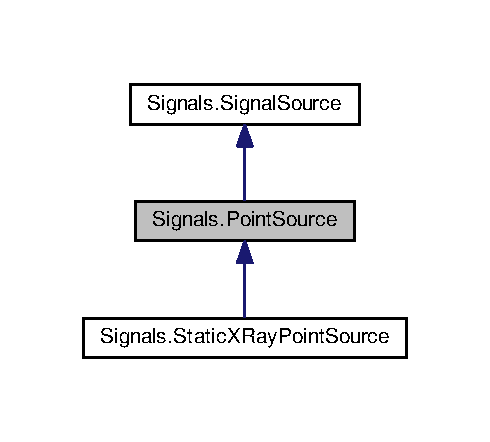
\includegraphics[width=235pt]{classSignals_1_1PointSource__inherit__graph}
\end{center}
\end{figure}


Collaboration diagram for Signals.\+Point\+Source\+:\nopagebreak
\begin{figure}[H]
\begin{center}
\leavevmode
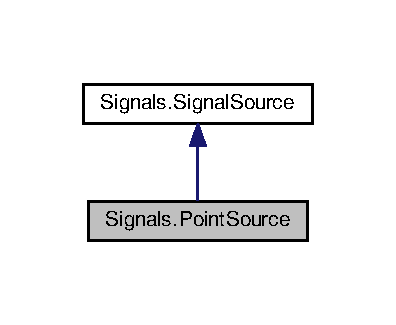
\includegraphics[width=190pt]{classSignals_1_1PointSource__coll__graph}
\end{center}
\end{figure}
\subsection*{Public Member Functions}
\begin{DoxyCompactItemize}
\item 
def {\bfseries \+\_\+\+\_\+init\+\_\+\+\_\+} (self, RA, D\+EC, attitude\+State\+Name=\textquotesingle{}attitude\textquotesingle{})\hypertarget{classSignals_1_1PointSource_a08c5c8fe52979814a725fac08b34c02f}{}\label{classSignals_1_1PointSource_a08c5c8fe52979814a725fac08b34c02f}

\item 
def {\bfseries Ra\+Dec} (self)\hypertarget{classSignals_1_1PointSource_a5fbb36eda0901536d77eff9a3262ae9e}{}\label{classSignals_1_1PointSource_a5fbb36eda0901536d77eff9a3262ae9e}

\item 
def {\bfseries compute\+Association\+Probability} (self, measurement, state\+Dict, validation\+Threshold=0)\hypertarget{classSignals_1_1PointSource_ab1389987fc68312eed77ae3126a21a2a}{}\label{classSignals_1_1PointSource_ab1389987fc68312eed77ae3126a21a2a}

\end{DoxyCompactItemize}
\subsection*{Public Attributes}
\begin{DoxyCompactItemize}
\item 
{\bfseries attitude\+State\+Name}\hypertarget{classSignals_1_1PointSource_a151f2600c3623d1ca49fb51feb8a1178}{}\label{classSignals_1_1PointSource_a151f2600c3623d1ca49fb51feb8a1178}

\end{DoxyCompactItemize}
\subsection*{Additional Inherited Members}


\subsection{Detailed Description}


Definition at line 18 of file Signals.\+py.



The documentation for this class was generated from the following file\+:\begin{DoxyCompactItemize}
\item 
Signals.\+py\end{DoxyCompactItemize}

\hypertarget{classSignals_1_1PoissonSource}{}\section{Signals.\+Poisson\+Source Class Reference}
\label{classSignals_1_1PoissonSource}\index{Signals.\+Poisson\+Source@{Signals.\+Poisson\+Source}}


Inheritance diagram for Signals.\+Poisson\+Source\+:\nopagebreak
\begin{figure}[H]
\begin{center}
\leavevmode
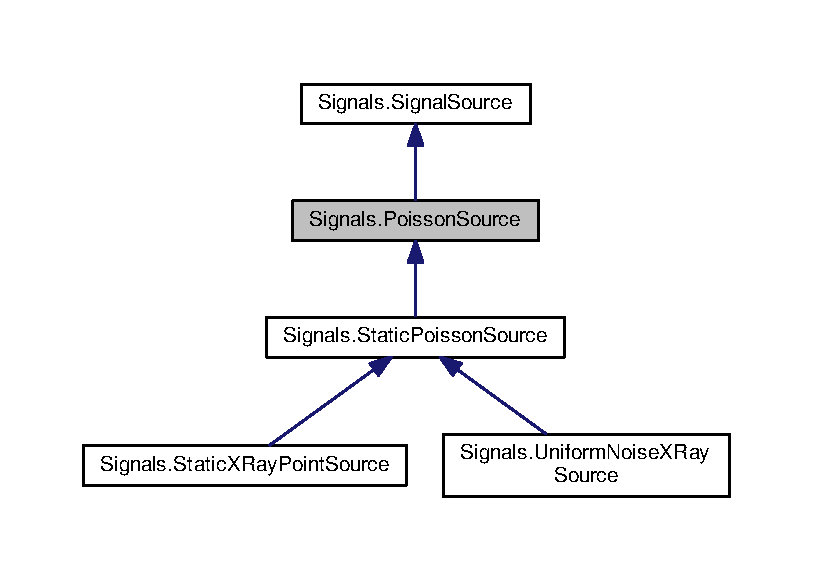
\includegraphics[width=350pt]{classSignals_1_1PoissonSource__inherit__graph}
\end{center}
\end{figure}


Collaboration diagram for Signals.\+Poisson\+Source\+:\nopagebreak
\begin{figure}[H]
\begin{center}
\leavevmode
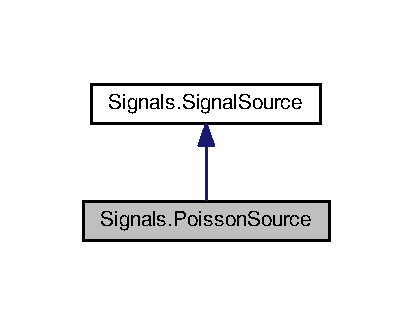
\includegraphics[width=198pt]{classSignals_1_1PoissonSource__coll__graph}
\end{center}
\end{figure}
\subsection*{Public Member Functions}
\begin{DoxyCompactItemize}
\item 
def \hyperlink{classSignals_1_1PoissonSource_a18f7e4d0f7f8385d195736a37fc0a445}{\+\_\+\+\_\+init\+\_\+\+\_\+} (self, \hyperlink{classSignals_1_1PoissonSource_a26e7bf25b1d9195bfded2a3ad6790bce}{flux})
\item 
def \hyperlink{classSignals_1_1PoissonSource_a8e7a6023e7ee53ed0b5b81c7d0aa361c}{compute\+Association\+Probability} (self, current\+Flux, measurement)
\item 
def \hyperlink{classSignals_1_1SignalSource_a85016cca8a7f1e188d314ced50577d05}{signal\+ID} (self)
\end{DoxyCompactItemize}
\subsection*{Public Attributes}
\begin{DoxyCompactItemize}
\item 
\hyperlink{classSignals_1_1PoissonSource_a66b0f3fb48cc130b6b07d7427092a522}{last\+Time}
\item 
\hyperlink{classSignals_1_1PoissonSource_a26e7bf25b1d9195bfded2a3ad6790bce}{flux}
\end{DoxyCompactItemize}
\subsection*{Static Public Attributes}
\begin{DoxyCompactItemize}
\item 
int \hyperlink{classSignals_1_1SignalSource_abcff0d069f17cb5ebe3eff15b6283a64}{next\+Signal\+ID} = 0
\end{DoxyCompactItemize}


\subsection{Detailed Description}


Definition at line 93 of file Signals.\+py.



\subsection{Constructor \& Destructor Documentation}
\index{Signals\+::\+Poisson\+Source@{Signals\+::\+Poisson\+Source}!\+\_\+\+\_\+init\+\_\+\+\_\+@{\+\_\+\+\_\+init\+\_\+\+\_\+}}
\index{\+\_\+\+\_\+init\+\_\+\+\_\+@{\+\_\+\+\_\+init\+\_\+\+\_\+}!Signals\+::\+Poisson\+Source@{Signals\+::\+Poisson\+Source}}
\subsubsection[{\texorpdfstring{\+\_\+\+\_\+init\+\_\+\+\_\+(self, flux)}{__init__(self, flux)}}]{\setlength{\rightskip}{0pt plus 5cm}def Signals.\+Poisson\+Source.\+\_\+\+\_\+init\+\_\+\+\_\+ (
\begin{DoxyParamCaption}
\item[{}]{self, }
\item[{}]{flux}
\end{DoxyParamCaption}
)}\hypertarget{classSignals_1_1PoissonSource_a18f7e4d0f7f8385d195736a37fc0a445}{}\label{classSignals_1_1PoissonSource_a18f7e4d0f7f8385d195736a37fc0a445}


Definition at line 97 of file Signals.\+py.



\subsection{Member Function Documentation}
\index{Signals\+::\+Poisson\+Source@{Signals\+::\+Poisson\+Source}!compute\+Association\+Probability@{compute\+Association\+Probability}}
\index{compute\+Association\+Probability@{compute\+Association\+Probability}!Signals\+::\+Poisson\+Source@{Signals\+::\+Poisson\+Source}}
\subsubsection[{\texorpdfstring{compute\+Association\+Probability(self, current\+Flux, measurement)}{computeAssociationProbability(self, currentFlux, measurement)}}]{\setlength{\rightskip}{0pt plus 5cm}def Signals.\+Poisson\+Source.\+compute\+Association\+Probability (
\begin{DoxyParamCaption}
\item[{}]{self, }
\item[{}]{current\+Flux, }
\item[{}]{measurement}
\end{DoxyParamCaption}
)}\hypertarget{classSignals_1_1PoissonSource_a8e7a6023e7ee53ed0b5b81c7d0aa361c}{}\label{classSignals_1_1PoissonSource_a8e7a6023e7ee53ed0b5b81c7d0aa361c}


Definition at line 107 of file Signals.\+py.

\index{Signals\+::\+Poisson\+Source@{Signals\+::\+Poisson\+Source}!signal\+ID@{signal\+ID}}
\index{signal\+ID@{signal\+ID}!Signals\+::\+Poisson\+Source@{Signals\+::\+Poisson\+Source}}
\subsubsection[{\texorpdfstring{signal\+I\+D(self)}{signalID(self)}}]{\setlength{\rightskip}{0pt plus 5cm}def Signals.\+Signal\+Source.\+signal\+ID (
\begin{DoxyParamCaption}
\item[{}]{self}
\end{DoxyParamCaption}
)\hspace{0.3cm}{\ttfamily [inherited]}}\hypertarget{classSignals_1_1SignalSource_a85016cca8a7f1e188d314ced50577d05}{}\label{classSignals_1_1SignalSource_a85016cca8a7f1e188d314ced50577d05}


Definition at line 14 of file Signals.\+py.



\subsection{Member Data Documentation}
\index{Signals\+::\+Poisson\+Source@{Signals\+::\+Poisson\+Source}!flux@{flux}}
\index{flux@{flux}!Signals\+::\+Poisson\+Source@{Signals\+::\+Poisson\+Source}}
\subsubsection[{\texorpdfstring{flux}{flux}}]{\setlength{\rightskip}{0pt plus 5cm}Signals.\+Poisson\+Source.\+flux}\hypertarget{classSignals_1_1PoissonSource_a26e7bf25b1d9195bfded2a3ad6790bce}{}\label{classSignals_1_1PoissonSource_a26e7bf25b1d9195bfded2a3ad6790bce}


Definition at line 100 of file Signals.\+py.

\index{Signals\+::\+Poisson\+Source@{Signals\+::\+Poisson\+Source}!last\+Time@{last\+Time}}
\index{last\+Time@{last\+Time}!Signals\+::\+Poisson\+Source@{Signals\+::\+Poisson\+Source}}
\subsubsection[{\texorpdfstring{last\+Time}{lastTime}}]{\setlength{\rightskip}{0pt plus 5cm}Signals.\+Poisson\+Source.\+last\+Time}\hypertarget{classSignals_1_1PoissonSource_a66b0f3fb48cc130b6b07d7427092a522}{}\label{classSignals_1_1PoissonSource_a66b0f3fb48cc130b6b07d7427092a522}


Definition at line 99 of file Signals.\+py.

\index{Signals\+::\+Poisson\+Source@{Signals\+::\+Poisson\+Source}!next\+Signal\+ID@{next\+Signal\+ID}}
\index{next\+Signal\+ID@{next\+Signal\+ID}!Signals\+::\+Poisson\+Source@{Signals\+::\+Poisson\+Source}}
\subsubsection[{\texorpdfstring{next\+Signal\+ID}{nextSignalID}}]{\setlength{\rightskip}{0pt plus 5cm}int Signals.\+Signal\+Source.\+next\+Signal\+ID = 0\hspace{0.3cm}{\ttfamily [static]}, {\ttfamily [inherited]}}\hypertarget{classSignals_1_1SignalSource_abcff0d069f17cb5ebe3eff15b6283a64}{}\label{classSignals_1_1SignalSource_abcff0d069f17cb5ebe3eff15b6283a64}


Definition at line 5 of file Signals.\+py.



The documentation for this class was generated from the following file\+:\begin{DoxyCompactItemize}
\item 
\hyperlink{Signals_8py}{Signals.\+py}\end{DoxyCompactItemize}

\hypertarget{classSignals_1_1SignalSource}{}\section{Signals.\+Signal\+Source Class Reference}
\label{classSignals_1_1SignalSource}\index{Signals.\+Signal\+Source@{Signals.\+Signal\+Source}}


Inheritance diagram for Signals.\+Signal\+Source\+:\nopagebreak
\begin{figure}[H]
\begin{center}
\leavevmode
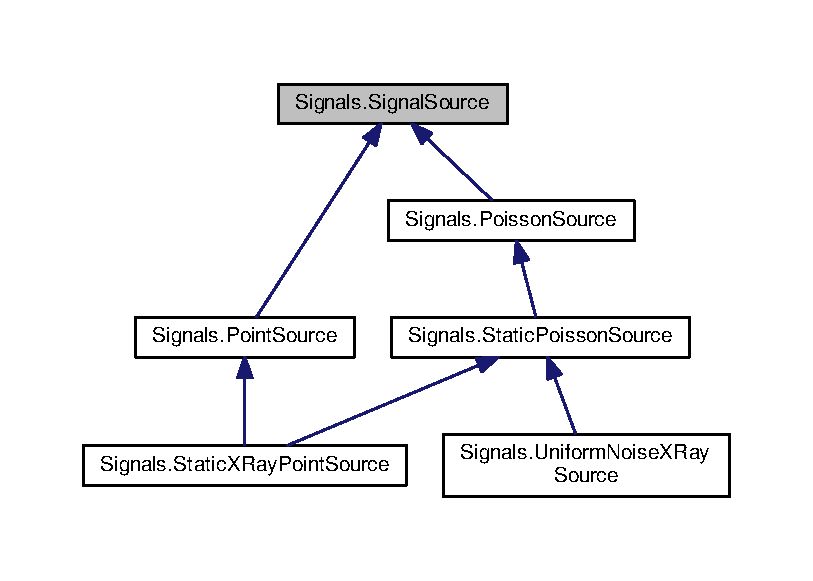
\includegraphics[width=350pt]{classSignals_1_1SignalSource__inherit__graph}
\end{center}
\end{figure}
\subsection*{Public Member Functions}
\begin{DoxyCompactItemize}
\item 
def \hyperlink{classSignals_1_1SignalSource_a18e58f799786c10300d066e9e0de7236}{\+\_\+\+\_\+init\+\_\+\+\_\+} (self)
\item 
def \hyperlink{classSignals_1_1SignalSource_a85016cca8a7f1e188d314ced50577d05}{signal\+ID} (self)
\end{DoxyCompactItemize}
\subsection*{Static Public Attributes}
\begin{DoxyCompactItemize}
\item 
int \hyperlink{classSignals_1_1SignalSource_abcff0d069f17cb5ebe3eff15b6283a64}{next\+Signal\+ID} = 0
\end{DoxyCompactItemize}
\subsection*{Private Attributes}
\begin{DoxyCompactItemize}
\item 
\hyperlink{classSignals_1_1SignalSource_a83c7d24dc35a94a5efaa2b6418b0f587}{\+\_\+\+\_\+signal\+I\+D\+\_\+\+\_\+}
\end{DoxyCompactItemize}


\subsection{Detailed Description}


Definition at line 4 of file Signals.\+py.



\subsection{Constructor \& Destructor Documentation}
\index{Signals\+::\+Signal\+Source@{Signals\+::\+Signal\+Source}!\+\_\+\+\_\+init\+\_\+\+\_\+@{\+\_\+\+\_\+init\+\_\+\+\_\+}}
\index{\+\_\+\+\_\+init\+\_\+\+\_\+@{\+\_\+\+\_\+init\+\_\+\+\_\+}!Signals\+::\+Signal\+Source@{Signals\+::\+Signal\+Source}}
\subsubsection[{\texorpdfstring{\+\_\+\+\_\+init\+\_\+\+\_\+(self)}{__init__(self)}}]{\setlength{\rightskip}{0pt plus 5cm}def Signals.\+Signal\+Source.\+\_\+\+\_\+init\+\_\+\+\_\+ (
\begin{DoxyParamCaption}
\item[{}]{self}
\end{DoxyParamCaption}
)}\hypertarget{classSignals_1_1SignalSource_a18e58f799786c10300d066e9e0de7236}{}\label{classSignals_1_1SignalSource_a18e58f799786c10300d066e9e0de7236}


Definition at line 9 of file Signals.\+py.



\subsection{Member Function Documentation}
\index{Signals\+::\+Signal\+Source@{Signals\+::\+Signal\+Source}!signal\+ID@{signal\+ID}}
\index{signal\+ID@{signal\+ID}!Signals\+::\+Signal\+Source@{Signals\+::\+Signal\+Source}}
\subsubsection[{\texorpdfstring{signal\+I\+D(self)}{signalID(self)}}]{\setlength{\rightskip}{0pt plus 5cm}def Signals.\+Signal\+Source.\+signal\+ID (
\begin{DoxyParamCaption}
\item[{}]{self}
\end{DoxyParamCaption}
)}\hypertarget{classSignals_1_1SignalSource_a85016cca8a7f1e188d314ced50577d05}{}\label{classSignals_1_1SignalSource_a85016cca8a7f1e188d314ced50577d05}


Definition at line 14 of file Signals.\+py.



\subsection{Member Data Documentation}
\index{Signals\+::\+Signal\+Source@{Signals\+::\+Signal\+Source}!\+\_\+\+\_\+signal\+I\+D\+\_\+\+\_\+@{\+\_\+\+\_\+signal\+I\+D\+\_\+\+\_\+}}
\index{\+\_\+\+\_\+signal\+I\+D\+\_\+\+\_\+@{\+\_\+\+\_\+signal\+I\+D\+\_\+\+\_\+}!Signals\+::\+Signal\+Source@{Signals\+::\+Signal\+Source}}
\subsubsection[{\texorpdfstring{\+\_\+\+\_\+signal\+I\+D\+\_\+\+\_\+}{__signalID__}}]{\setlength{\rightskip}{0pt plus 5cm}Signals.\+Signal\+Source.\+\_\+\+\_\+signal\+I\+D\+\_\+\+\_\+\hspace{0.3cm}{\ttfamily [private]}}\hypertarget{classSignals_1_1SignalSource_a83c7d24dc35a94a5efaa2b6418b0f587}{}\label{classSignals_1_1SignalSource_a83c7d24dc35a94a5efaa2b6418b0f587}


Definition at line 10 of file Signals.\+py.

\index{Signals\+::\+Signal\+Source@{Signals\+::\+Signal\+Source}!next\+Signal\+ID@{next\+Signal\+ID}}
\index{next\+Signal\+ID@{next\+Signal\+ID}!Signals\+::\+Signal\+Source@{Signals\+::\+Signal\+Source}}
\subsubsection[{\texorpdfstring{next\+Signal\+ID}{nextSignalID}}]{\setlength{\rightskip}{0pt plus 5cm}int Signals.\+Signal\+Source.\+next\+Signal\+ID = 0\hspace{0.3cm}{\ttfamily [static]}}\hypertarget{classSignals_1_1SignalSource_abcff0d069f17cb5ebe3eff15b6283a64}{}\label{classSignals_1_1SignalSource_abcff0d069f17cb5ebe3eff15b6283a64}


Definition at line 5 of file Signals.\+py.



The documentation for this class was generated from the following file\+:\begin{DoxyCompactItemize}
\item 
\hyperlink{Signals_8py}{Signals.\+py}\end{DoxyCompactItemize}

\hypertarget{classSignals_1_1StaticPoissonSource}{}\section{Signals.\+Static\+Poisson\+Source Class Reference}
\label{classSignals_1_1StaticPoissonSource}\index{Signals.\+Static\+Poisson\+Source@{Signals.\+Static\+Poisson\+Source}}


Inheritance diagram for Signals.\+Static\+Poisson\+Source\+:\nopagebreak
\begin{figure}[H]
\begin{center}
\leavevmode
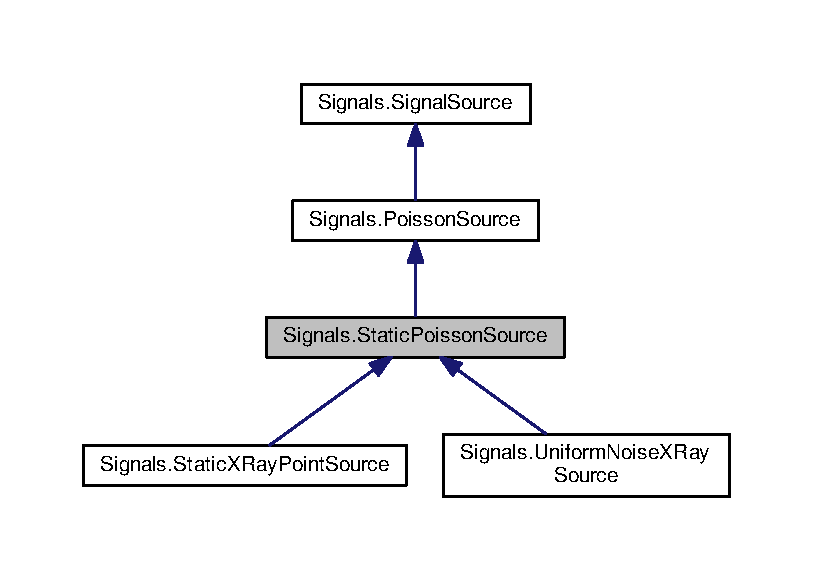
\includegraphics[width=350pt]{classSignals_1_1StaticPoissonSource__inherit__graph}
\end{center}
\end{figure}


Collaboration diagram for Signals.\+Static\+Poisson\+Source\+:\nopagebreak
\begin{figure}[H]
\begin{center}
\leavevmode
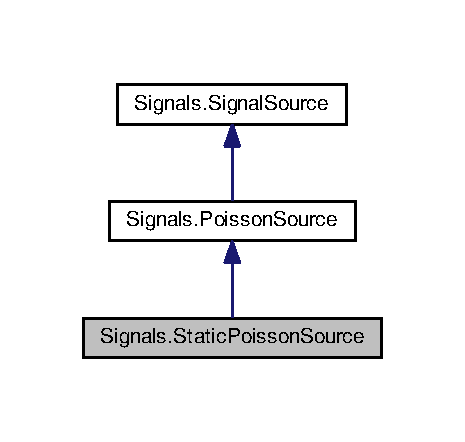
\includegraphics[width=223pt]{classSignals_1_1StaticPoissonSource__coll__graph}
\end{center}
\end{figure}
\subsection*{Public Member Functions}
\begin{DoxyCompactItemize}
\item 
def \hyperlink{classSignals_1_1StaticPoissonSource_a71ff9a86dc2d7e1a89e5f40e0de5f20e}{\+\_\+\+\_\+init\+\_\+\+\_\+} (self, \hyperlink{classSignals_1_1PoissonSource_a26e7bf25b1d9195bfded2a3ad6790bce}{flux})
\item 
def \hyperlink{classSignals_1_1StaticPoissonSource_a61351ebf4f75f28e227cfee7ca7e5d64}{compute\+Association\+Probability} (self, measurement)
\item 
def \hyperlink{classSignals_1_1PoissonSource_a8e7a6023e7ee53ed0b5b81c7d0aa361c}{compute\+Association\+Probability} (self, current\+Flux, measurement)
\item 
def \hyperlink{classSignals_1_1SignalSource_a85016cca8a7f1e188d314ced50577d05}{signal\+ID} (self)
\end{DoxyCompactItemize}
\subsection*{Public Attributes}
\begin{DoxyCompactItemize}
\item 
\hyperlink{classSignals_1_1PoissonSource_a66b0f3fb48cc130b6b07d7427092a522}{last\+Time}
\item 
\hyperlink{classSignals_1_1PoissonSource_a26e7bf25b1d9195bfded2a3ad6790bce}{flux}
\end{DoxyCompactItemize}
\subsection*{Static Public Attributes}
\begin{DoxyCompactItemize}
\item 
int \hyperlink{classSignals_1_1SignalSource_abcff0d069f17cb5ebe3eff15b6283a64}{next\+Signal\+ID} = 0
\end{DoxyCompactItemize}


\subsection{Detailed Description}


Definition at line 114 of file Signals.\+py.



\subsection{Constructor \& Destructor Documentation}
\index{Signals\+::\+Static\+Poisson\+Source@{Signals\+::\+Static\+Poisson\+Source}!\+\_\+\+\_\+init\+\_\+\+\_\+@{\+\_\+\+\_\+init\+\_\+\+\_\+}}
\index{\+\_\+\+\_\+init\+\_\+\+\_\+@{\+\_\+\+\_\+init\+\_\+\+\_\+}!Signals\+::\+Static\+Poisson\+Source@{Signals\+::\+Static\+Poisson\+Source}}
\subsubsection[{\texorpdfstring{\+\_\+\+\_\+init\+\_\+\+\_\+(self, flux)}{__init__(self, flux)}}]{\setlength{\rightskip}{0pt plus 5cm}def Signals.\+Static\+Poisson\+Source.\+\_\+\+\_\+init\+\_\+\+\_\+ (
\begin{DoxyParamCaption}
\item[{}]{self, }
\item[{}]{flux}
\end{DoxyParamCaption}
)}\hypertarget{classSignals_1_1StaticPoissonSource_a71ff9a86dc2d7e1a89e5f40e0de5f20e}{}\label{classSignals_1_1StaticPoissonSource_a71ff9a86dc2d7e1a89e5f40e0de5f20e}


Definition at line 118 of file Signals.\+py.



\subsection{Member Function Documentation}
\index{Signals\+::\+Static\+Poisson\+Source@{Signals\+::\+Static\+Poisson\+Source}!compute\+Association\+Probability@{compute\+Association\+Probability}}
\index{compute\+Association\+Probability@{compute\+Association\+Probability}!Signals\+::\+Static\+Poisson\+Source@{Signals\+::\+Static\+Poisson\+Source}}
\subsubsection[{\texorpdfstring{compute\+Association\+Probability(self, current\+Flux, measurement)}{computeAssociationProbability(self, currentFlux, measurement)}}]{\setlength{\rightskip}{0pt plus 5cm}def Signals.\+Poisson\+Source.\+compute\+Association\+Probability (
\begin{DoxyParamCaption}
\item[{}]{self, }
\item[{}]{current\+Flux, }
\item[{}]{measurement}
\end{DoxyParamCaption}
)\hspace{0.3cm}{\ttfamily [inherited]}}\hypertarget{classSignals_1_1PoissonSource_a8e7a6023e7ee53ed0b5b81c7d0aa361c}{}\label{classSignals_1_1PoissonSource_a8e7a6023e7ee53ed0b5b81c7d0aa361c}


Definition at line 107 of file Signals.\+py.

\index{Signals\+::\+Static\+Poisson\+Source@{Signals\+::\+Static\+Poisson\+Source}!compute\+Association\+Probability@{compute\+Association\+Probability}}
\index{compute\+Association\+Probability@{compute\+Association\+Probability}!Signals\+::\+Static\+Poisson\+Source@{Signals\+::\+Static\+Poisson\+Source}}
\subsubsection[{\texorpdfstring{compute\+Association\+Probability(self, measurement)}{computeAssociationProbability(self, measurement)}}]{\setlength{\rightskip}{0pt plus 5cm}def Signals.\+Static\+Poisson\+Source.\+compute\+Association\+Probability (
\begin{DoxyParamCaption}
\item[{}]{self, }
\item[{}]{measurement}
\end{DoxyParamCaption}
)}\hypertarget{classSignals_1_1StaticPoissonSource_a61351ebf4f75f28e227cfee7ca7e5d64}{}\label{classSignals_1_1StaticPoissonSource_a61351ebf4f75f28e227cfee7ca7e5d64}


Definition at line 124 of file Signals.\+py.

\index{Signals\+::\+Static\+Poisson\+Source@{Signals\+::\+Static\+Poisson\+Source}!signal\+ID@{signal\+ID}}
\index{signal\+ID@{signal\+ID}!Signals\+::\+Static\+Poisson\+Source@{Signals\+::\+Static\+Poisson\+Source}}
\subsubsection[{\texorpdfstring{signal\+I\+D(self)}{signalID(self)}}]{\setlength{\rightskip}{0pt plus 5cm}def Signals.\+Signal\+Source.\+signal\+ID (
\begin{DoxyParamCaption}
\item[{}]{self}
\end{DoxyParamCaption}
)\hspace{0.3cm}{\ttfamily [inherited]}}\hypertarget{classSignals_1_1SignalSource_a85016cca8a7f1e188d314ced50577d05}{}\label{classSignals_1_1SignalSource_a85016cca8a7f1e188d314ced50577d05}


Definition at line 14 of file Signals.\+py.



\subsection{Member Data Documentation}
\index{Signals\+::\+Static\+Poisson\+Source@{Signals\+::\+Static\+Poisson\+Source}!flux@{flux}}
\index{flux@{flux}!Signals\+::\+Static\+Poisson\+Source@{Signals\+::\+Static\+Poisson\+Source}}
\subsubsection[{\texorpdfstring{flux}{flux}}]{\setlength{\rightskip}{0pt plus 5cm}Signals.\+Poisson\+Source.\+flux\hspace{0.3cm}{\ttfamily [inherited]}}\hypertarget{classSignals_1_1PoissonSource_a26e7bf25b1d9195bfded2a3ad6790bce}{}\label{classSignals_1_1PoissonSource_a26e7bf25b1d9195bfded2a3ad6790bce}


Definition at line 100 of file Signals.\+py.

\index{Signals\+::\+Static\+Poisson\+Source@{Signals\+::\+Static\+Poisson\+Source}!last\+Time@{last\+Time}}
\index{last\+Time@{last\+Time}!Signals\+::\+Static\+Poisson\+Source@{Signals\+::\+Static\+Poisson\+Source}}
\subsubsection[{\texorpdfstring{last\+Time}{lastTime}}]{\setlength{\rightskip}{0pt plus 5cm}Signals.\+Poisson\+Source.\+last\+Time\hspace{0.3cm}{\ttfamily [inherited]}}\hypertarget{classSignals_1_1PoissonSource_a66b0f3fb48cc130b6b07d7427092a522}{}\label{classSignals_1_1PoissonSource_a66b0f3fb48cc130b6b07d7427092a522}


Definition at line 99 of file Signals.\+py.

\index{Signals\+::\+Static\+Poisson\+Source@{Signals\+::\+Static\+Poisson\+Source}!next\+Signal\+ID@{next\+Signal\+ID}}
\index{next\+Signal\+ID@{next\+Signal\+ID}!Signals\+::\+Static\+Poisson\+Source@{Signals\+::\+Static\+Poisson\+Source}}
\subsubsection[{\texorpdfstring{next\+Signal\+ID}{nextSignalID}}]{\setlength{\rightskip}{0pt plus 5cm}int Signals.\+Signal\+Source.\+next\+Signal\+ID = 0\hspace{0.3cm}{\ttfamily [static]}, {\ttfamily [inherited]}}\hypertarget{classSignals_1_1SignalSource_abcff0d069f17cb5ebe3eff15b6283a64}{}\label{classSignals_1_1SignalSource_abcff0d069f17cb5ebe3eff15b6283a64}


Definition at line 5 of file Signals.\+py.



The documentation for this class was generated from the following file\+:\begin{DoxyCompactItemize}
\item 
\hyperlink{Signals_8py}{Signals.\+py}\end{DoxyCompactItemize}

\hypertarget{classSignals_1_1StaticXRayPointSource}{}\section{Signals.\+Static\+X\+Ray\+Point\+Source Class Reference}
\label{classSignals_1_1StaticXRayPointSource}\index{Signals.\+Static\+X\+Ray\+Point\+Source@{Signals.\+Static\+X\+Ray\+Point\+Source}}


Inheritance diagram for Signals.\+Static\+X\+Ray\+Point\+Source\+:\nopagebreak
\begin{figure}[H]
\begin{center}
\leavevmode
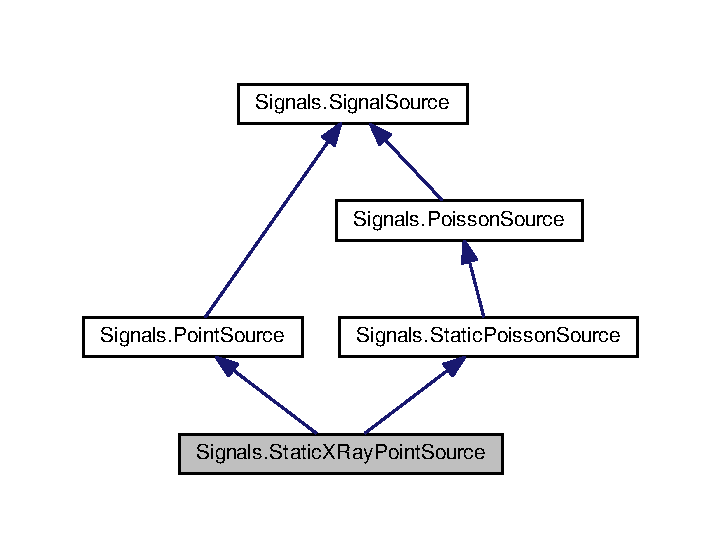
\includegraphics[width=346pt]{classSignals_1_1StaticXRayPointSource__inherit__graph}
\end{center}
\end{figure}


Collaboration diagram for Signals.\+Static\+X\+Ray\+Point\+Source\+:\nopagebreak
\begin{figure}[H]
\begin{center}
\leavevmode
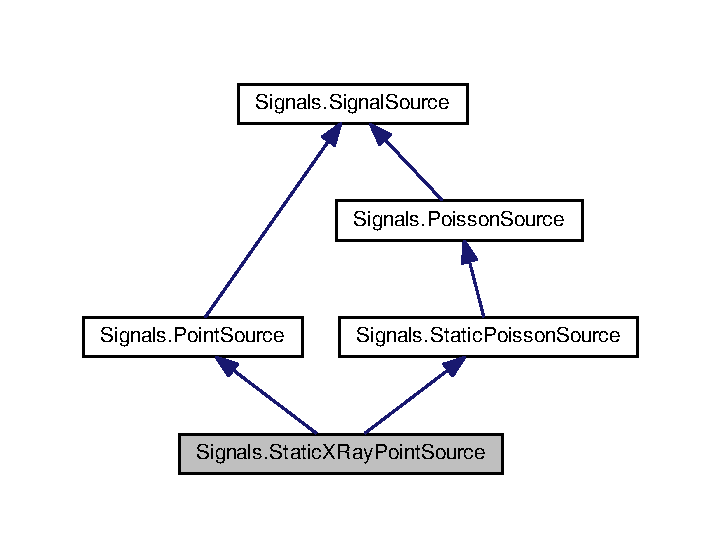
\includegraphics[width=346pt]{classSignals_1_1StaticXRayPointSource__coll__graph}
\end{center}
\end{figure}
\subsection*{Public Member Functions}
\begin{DoxyCompactItemize}
\item 
def \hyperlink{classSignals_1_1StaticXRayPointSource_ae3efcdb0e8a8c7fe9e3984c1cb785196}{\+\_\+\+\_\+init\+\_\+\+\_\+} (self, RA, D\+EC, \hyperlink{classSignals_1_1StaticXRayPointSource_a7e16da6506ee1b83c9858dce9c7856ea}{peak\+Photon\+Flux}, \hyperlink{classSignals_1_1PointSource_a151f2600c3623d1ca49fb51feb8a1178}{attitude\+State\+Name}=\textquotesingle{}attitude\textquotesingle{})
\item 
def \hyperlink{classSignals_1_1StaticXRayPointSource_a0533a3647597c6ad91c238ab2b97a829}{compute\+Association\+Probability} (self, measurement, state\+Dict, validation\+Threshold=0)
\item 
def \hyperlink{classSignals_1_1PointSource_a5fbb36eda0901536d77eff9a3262ae9e}{Ra\+Dec} (self)
\item 
def \hyperlink{classSignals_1_1PointSource_aec5f944753a4c097e99da175ec848a92}{unit\+Vec} (self, \hyperlink{classSignals_1_1PointSource_a5fbb36eda0901536d77eff9a3262ae9e}{Ra\+Dec})
\item 
def \hyperlink{classSignals_1_1SignalSource_a85016cca8a7f1e188d314ced50577d05}{signal\+ID} (self)
\item 
def \hyperlink{classSignals_1_1StaticPoissonSource_a61351ebf4f75f28e227cfee7ca7e5d64}{compute\+Association\+Probability} (self, measurement)
\item 
def \hyperlink{classSignals_1_1PoissonSource_a8e7a6023e7ee53ed0b5b81c7d0aa361c}{compute\+Association\+Probability} (self, current\+Flux, measurement)
\item 
def \hyperlink{classSignals_1_1SignalSource_a85016cca8a7f1e188d314ced50577d05}{signal\+ID} (self)
\end{DoxyCompactItemize}
\subsection*{Public Attributes}
\begin{DoxyCompactItemize}
\item 
\hyperlink{classSignals_1_1StaticXRayPointSource_a7e16da6506ee1b83c9858dce9c7856ea}{peak\+Photon\+Flux}
\item 
\hyperlink{classSignals_1_1PointSource_a151f2600c3623d1ca49fb51feb8a1178}{attitude\+State\+Name}
\item 
\hyperlink{classSignals_1_1PoissonSource_a66b0f3fb48cc130b6b07d7427092a522}{last\+Time}
\item 
\hyperlink{classSignals_1_1PoissonSource_a26e7bf25b1d9195bfded2a3ad6790bce}{flux}
\end{DoxyCompactItemize}
\subsection*{Static Public Attributes}
\begin{DoxyCompactItemize}
\item 
int \hyperlink{classSignals_1_1SignalSource_abcff0d069f17cb5ebe3eff15b6283a64}{next\+Signal\+ID} = 0
\item 
int \hyperlink{classSignals_1_1SignalSource_abcff0d069f17cb5ebe3eff15b6283a64}{next\+Signal\+ID} = 0
\end{DoxyCompactItemize}


\subsection{Detailed Description}


Definition at line 155 of file Signals.\+py.



\subsection{Constructor \& Destructor Documentation}
\index{Signals\+::\+Static\+X\+Ray\+Point\+Source@{Signals\+::\+Static\+X\+Ray\+Point\+Source}!\+\_\+\+\_\+init\+\_\+\+\_\+@{\+\_\+\+\_\+init\+\_\+\+\_\+}}
\index{\+\_\+\+\_\+init\+\_\+\+\_\+@{\+\_\+\+\_\+init\+\_\+\+\_\+}!Signals\+::\+Static\+X\+Ray\+Point\+Source@{Signals\+::\+Static\+X\+Ray\+Point\+Source}}
\subsubsection[{\texorpdfstring{\+\_\+\+\_\+init\+\_\+\+\_\+(self, R\+A, D\+E\+C, peak\+Photon\+Flux, attitude\+State\+Name=\textquotesingle{}attitude\textquotesingle{})}{__init__(self, RA, DEC, peakPhotonFlux, attitudeStateName='attitude')}}]{\setlength{\rightskip}{0pt plus 5cm}def Signals.\+Static\+X\+Ray\+Point\+Source.\+\_\+\+\_\+init\+\_\+\+\_\+ (
\begin{DoxyParamCaption}
\item[{}]{self, }
\item[{}]{RA, }
\item[{}]{D\+EC, }
\item[{}]{peak\+Photon\+Flux, }
\item[{}]{attitude\+State\+Name = {\ttfamily \textquotesingle{}attitude\textquotesingle{}}}
\end{DoxyParamCaption}
)}\hypertarget{classSignals_1_1StaticXRayPointSource_ae3efcdb0e8a8c7fe9e3984c1cb785196}{}\label{classSignals_1_1StaticXRayPointSource_ae3efcdb0e8a8c7fe9e3984c1cb785196}


Definition at line 163 of file Signals.\+py.



\subsection{Member Function Documentation}
\index{Signals\+::\+Static\+X\+Ray\+Point\+Source@{Signals\+::\+Static\+X\+Ray\+Point\+Source}!compute\+Association\+Probability@{compute\+Association\+Probability}}
\index{compute\+Association\+Probability@{compute\+Association\+Probability}!Signals\+::\+Static\+X\+Ray\+Point\+Source@{Signals\+::\+Static\+X\+Ray\+Point\+Source}}
\subsubsection[{\texorpdfstring{compute\+Association\+Probability(self, current\+Flux, measurement)}{computeAssociationProbability(self, currentFlux, measurement)}}]{\setlength{\rightskip}{0pt plus 5cm}def Signals.\+Poisson\+Source.\+compute\+Association\+Probability (
\begin{DoxyParamCaption}
\item[{}]{self, }
\item[{}]{current\+Flux, }
\item[{}]{measurement}
\end{DoxyParamCaption}
)\hspace{0.3cm}{\ttfamily [inherited]}}\hypertarget{classSignals_1_1PoissonSource_a8e7a6023e7ee53ed0b5b81c7d0aa361c}{}\label{classSignals_1_1PoissonSource_a8e7a6023e7ee53ed0b5b81c7d0aa361c}


Definition at line 117 of file Signals.\+py.

\index{Signals\+::\+Static\+X\+Ray\+Point\+Source@{Signals\+::\+Static\+X\+Ray\+Point\+Source}!compute\+Association\+Probability@{compute\+Association\+Probability}}
\index{compute\+Association\+Probability@{compute\+Association\+Probability}!Signals\+::\+Static\+X\+Ray\+Point\+Source@{Signals\+::\+Static\+X\+Ray\+Point\+Source}}
\subsubsection[{\texorpdfstring{compute\+Association\+Probability(self, measurement)}{computeAssociationProbability(self, measurement)}}]{\setlength{\rightskip}{0pt plus 5cm}def Signals.\+Static\+Poisson\+Source.\+compute\+Association\+Probability (
\begin{DoxyParamCaption}
\item[{}]{self, }
\item[{}]{measurement}
\end{DoxyParamCaption}
)\hspace{0.3cm}{\ttfamily [inherited]}}\hypertarget{classSignals_1_1StaticPoissonSource_a61351ebf4f75f28e227cfee7ca7e5d64}{}\label{classSignals_1_1StaticPoissonSource_a61351ebf4f75f28e227cfee7ca7e5d64}


Definition at line 134 of file Signals.\+py.

\index{Signals\+::\+Static\+X\+Ray\+Point\+Source@{Signals\+::\+Static\+X\+Ray\+Point\+Source}!compute\+Association\+Probability@{compute\+Association\+Probability}}
\index{compute\+Association\+Probability@{compute\+Association\+Probability}!Signals\+::\+Static\+X\+Ray\+Point\+Source@{Signals\+::\+Static\+X\+Ray\+Point\+Source}}
\subsubsection[{\texorpdfstring{compute\+Association\+Probability(self, measurement, state\+Dict, validation\+Threshold=0)}{computeAssociationProbability(self, measurement, stateDict, validationThreshold=0)}}]{\setlength{\rightskip}{0pt plus 5cm}def Signals.\+Static\+X\+Ray\+Point\+Source.\+compute\+Association\+Probability (
\begin{DoxyParamCaption}
\item[{}]{self, }
\item[{}]{measurement, }
\item[{}]{state\+Dict, }
\item[{}]{validation\+Threshold = {\ttfamily 0}}
\end{DoxyParamCaption}
)}\hypertarget{classSignals_1_1StaticXRayPointSource_a0533a3647597c6ad91c238ab2b97a829}{}\label{classSignals_1_1StaticXRayPointSource_a0533a3647597c6ad91c238ab2b97a829}


Definition at line 176 of file Signals.\+py.

\index{Signals\+::\+Static\+X\+Ray\+Point\+Source@{Signals\+::\+Static\+X\+Ray\+Point\+Source}!Ra\+Dec@{Ra\+Dec}}
\index{Ra\+Dec@{Ra\+Dec}!Signals\+::\+Static\+X\+Ray\+Point\+Source@{Signals\+::\+Static\+X\+Ray\+Point\+Source}}
\subsubsection[{\texorpdfstring{Ra\+Dec(self)}{RaDec(self)}}]{\setlength{\rightskip}{0pt plus 5cm}def Signals.\+Point\+Source.\+Ra\+Dec (
\begin{DoxyParamCaption}
\item[{}]{self}
\end{DoxyParamCaption}
)\hspace{0.3cm}{\ttfamily [inherited]}}\hypertarget{classSignals_1_1PointSource_a5fbb36eda0901536d77eff9a3262ae9e}{}\label{classSignals_1_1PointSource_a5fbb36eda0901536d77eff9a3262ae9e}


Definition at line 33 of file Signals.\+py.

\index{Signals\+::\+Static\+X\+Ray\+Point\+Source@{Signals\+::\+Static\+X\+Ray\+Point\+Source}!signal\+ID@{signal\+ID}}
\index{signal\+ID@{signal\+ID}!Signals\+::\+Static\+X\+Ray\+Point\+Source@{Signals\+::\+Static\+X\+Ray\+Point\+Source}}
\subsubsection[{\texorpdfstring{signal\+I\+D(self)}{signalID(self)}}]{\setlength{\rightskip}{0pt plus 5cm}def Signals.\+Signal\+Source.\+signal\+ID (
\begin{DoxyParamCaption}
\item[{}]{self}
\end{DoxyParamCaption}
)\hspace{0.3cm}{\ttfamily [inherited]}}\hypertarget{classSignals_1_1SignalSource_a85016cca8a7f1e188d314ced50577d05}{}\label{classSignals_1_1SignalSource_a85016cca8a7f1e188d314ced50577d05}


Definition at line 14 of file Signals.\+py.

\index{Signals\+::\+Static\+X\+Ray\+Point\+Source@{Signals\+::\+Static\+X\+Ray\+Point\+Source}!signal\+ID@{signal\+ID}}
\index{signal\+ID@{signal\+ID}!Signals\+::\+Static\+X\+Ray\+Point\+Source@{Signals\+::\+Static\+X\+Ray\+Point\+Source}}
\subsubsection[{\texorpdfstring{signal\+I\+D(self)}{signalID(self)}}]{\setlength{\rightskip}{0pt plus 5cm}def Signals.\+Signal\+Source.\+signal\+ID (
\begin{DoxyParamCaption}
\item[{}]{self}
\end{DoxyParamCaption}
)\hspace{0.3cm}{\ttfamily [inherited]}}\hypertarget{classSignals_1_1SignalSource_a85016cca8a7f1e188d314ced50577d05}{}\label{classSignals_1_1SignalSource_a85016cca8a7f1e188d314ced50577d05}


Definition at line 14 of file Signals.\+py.

\index{Signals\+::\+Static\+X\+Ray\+Point\+Source@{Signals\+::\+Static\+X\+Ray\+Point\+Source}!unit\+Vec@{unit\+Vec}}
\index{unit\+Vec@{unit\+Vec}!Signals\+::\+Static\+X\+Ray\+Point\+Source@{Signals\+::\+Static\+X\+Ray\+Point\+Source}}
\subsubsection[{\texorpdfstring{unit\+Vec(self, Ra\+Dec)}{unitVec(self, RaDec)}}]{\setlength{\rightskip}{0pt plus 5cm}def Signals.\+Point\+Source.\+unit\+Vec (
\begin{DoxyParamCaption}
\item[{}]{self, }
\item[{}]{Ra\+Dec}
\end{DoxyParamCaption}
)\hspace{0.3cm}{\ttfamily [inherited]}}\hypertarget{classSignals_1_1PointSource_aec5f944753a4c097e99da175ec848a92}{}\label{classSignals_1_1PointSource_aec5f944753a4c097e99da175ec848a92}


Definition at line 38 of file Signals.\+py.



\subsection{Member Data Documentation}
\index{Signals\+::\+Static\+X\+Ray\+Point\+Source@{Signals\+::\+Static\+X\+Ray\+Point\+Source}!attitude\+State\+Name@{attitude\+State\+Name}}
\index{attitude\+State\+Name@{attitude\+State\+Name}!Signals\+::\+Static\+X\+Ray\+Point\+Source@{Signals\+::\+Static\+X\+Ray\+Point\+Source}}
\subsubsection[{\texorpdfstring{attitude\+State\+Name}{attitudeStateName}}]{\setlength{\rightskip}{0pt plus 5cm}Signals.\+Point\+Source.\+attitude\+State\+Name\hspace{0.3cm}{\ttfamily [inherited]}}\hypertarget{classSignals_1_1PointSource_a151f2600c3623d1ca49fb51feb8a1178}{}\label{classSignals_1_1PointSource_a151f2600c3623d1ca49fb51feb8a1178}


Definition at line 29 of file Signals.\+py.

\index{Signals\+::\+Static\+X\+Ray\+Point\+Source@{Signals\+::\+Static\+X\+Ray\+Point\+Source}!flux@{flux}}
\index{flux@{flux}!Signals\+::\+Static\+X\+Ray\+Point\+Source@{Signals\+::\+Static\+X\+Ray\+Point\+Source}}
\subsubsection[{\texorpdfstring{flux}{flux}}]{\setlength{\rightskip}{0pt plus 5cm}Signals.\+Poisson\+Source.\+flux\hspace{0.3cm}{\ttfamily [inherited]}}\hypertarget{classSignals_1_1PoissonSource_a26e7bf25b1d9195bfded2a3ad6790bce}{}\label{classSignals_1_1PoissonSource_a26e7bf25b1d9195bfded2a3ad6790bce}


Definition at line 110 of file Signals.\+py.

\index{Signals\+::\+Static\+X\+Ray\+Point\+Source@{Signals\+::\+Static\+X\+Ray\+Point\+Source}!last\+Time@{last\+Time}}
\index{last\+Time@{last\+Time}!Signals\+::\+Static\+X\+Ray\+Point\+Source@{Signals\+::\+Static\+X\+Ray\+Point\+Source}}
\subsubsection[{\texorpdfstring{last\+Time}{lastTime}}]{\setlength{\rightskip}{0pt plus 5cm}Signals.\+Poisson\+Source.\+last\+Time\hspace{0.3cm}{\ttfamily [inherited]}}\hypertarget{classSignals_1_1PoissonSource_a66b0f3fb48cc130b6b07d7427092a522}{}\label{classSignals_1_1PoissonSource_a66b0f3fb48cc130b6b07d7427092a522}


Definition at line 109 of file Signals.\+py.

\index{Signals\+::\+Static\+X\+Ray\+Point\+Source@{Signals\+::\+Static\+X\+Ray\+Point\+Source}!next\+Signal\+ID@{next\+Signal\+ID}}
\index{next\+Signal\+ID@{next\+Signal\+ID}!Signals\+::\+Static\+X\+Ray\+Point\+Source@{Signals\+::\+Static\+X\+Ray\+Point\+Source}}
\subsubsection[{\texorpdfstring{next\+Signal\+ID}{nextSignalID}}]{\setlength{\rightskip}{0pt plus 5cm}int Signals.\+Signal\+Source.\+next\+Signal\+ID = 0\hspace{0.3cm}{\ttfamily [static]}, {\ttfamily [inherited]}}\hypertarget{classSignals_1_1SignalSource_abcff0d069f17cb5ebe3eff15b6283a64}{}\label{classSignals_1_1SignalSource_abcff0d069f17cb5ebe3eff15b6283a64}


Definition at line 5 of file Signals.\+py.

\index{Signals\+::\+Static\+X\+Ray\+Point\+Source@{Signals\+::\+Static\+X\+Ray\+Point\+Source}!next\+Signal\+ID@{next\+Signal\+ID}}
\index{next\+Signal\+ID@{next\+Signal\+ID}!Signals\+::\+Static\+X\+Ray\+Point\+Source@{Signals\+::\+Static\+X\+Ray\+Point\+Source}}
\subsubsection[{\texorpdfstring{next\+Signal\+ID}{nextSignalID}}]{\setlength{\rightskip}{0pt plus 5cm}int Signals.\+Signal\+Source.\+next\+Signal\+ID = 0\hspace{0.3cm}{\ttfamily [static]}, {\ttfamily [inherited]}}\hypertarget{classSignals_1_1SignalSource_abcff0d069f17cb5ebe3eff15b6283a64}{}\label{classSignals_1_1SignalSource_abcff0d069f17cb5ebe3eff15b6283a64}


Definition at line 5 of file Signals.\+py.

\index{Signals\+::\+Static\+X\+Ray\+Point\+Source@{Signals\+::\+Static\+X\+Ray\+Point\+Source}!peak\+Photon\+Flux@{peak\+Photon\+Flux}}
\index{peak\+Photon\+Flux@{peak\+Photon\+Flux}!Signals\+::\+Static\+X\+Ray\+Point\+Source@{Signals\+::\+Static\+X\+Ray\+Point\+Source}}
\subsubsection[{\texorpdfstring{peak\+Photon\+Flux}{peakPhotonFlux}}]{\setlength{\rightskip}{0pt plus 5cm}Signals.\+Static\+X\+Ray\+Point\+Source.\+peak\+Photon\+Flux}\hypertarget{classSignals_1_1StaticXRayPointSource_a7e16da6506ee1b83c9858dce9c7856ea}{}\label{classSignals_1_1StaticXRayPointSource_a7e16da6506ee1b83c9858dce9c7856ea}


Definition at line 167 of file Signals.\+py.



The documentation for this class was generated from the following file\+:\begin{DoxyCompactItemize}
\item 
\hyperlink{Signals_8py}{Signals.\+py}\end{DoxyCompactItemize}

\hypertarget{classSignals_1_1UniformNoiseXRaySource}{}\section{Signals.\+Uniform\+Noise\+X\+Ray\+Source Class Reference}
\label{classSignals_1_1UniformNoiseXRaySource}\index{Signals.\+Uniform\+Noise\+X\+Ray\+Source@{Signals.\+Uniform\+Noise\+X\+Ray\+Source}}


Inheritance diagram for Signals.\+Uniform\+Noise\+X\+Ray\+Source\+:\nopagebreak
\begin{figure}[H]
\begin{center}
\leavevmode
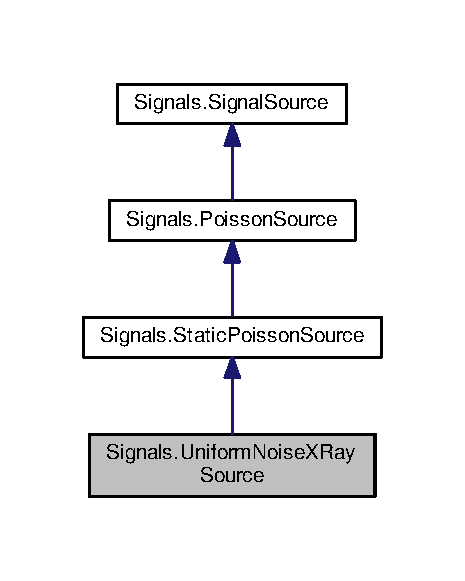
\includegraphics[width=223pt]{classSignals_1_1UniformNoiseXRaySource__inherit__graph}
\end{center}
\end{figure}


Collaboration diagram for Signals.\+Uniform\+Noise\+X\+Ray\+Source\+:\nopagebreak
\begin{figure}[H]
\begin{center}
\leavevmode
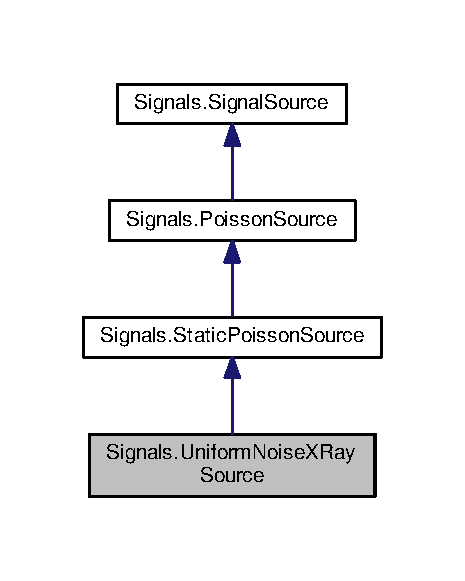
\includegraphics[width=223pt]{classSignals_1_1UniformNoiseXRaySource__coll__graph}
\end{center}
\end{figure}
\subsection*{Public Member Functions}
\begin{DoxyCompactItemize}
\item 
def \hyperlink{classSignals_1_1UniformNoiseXRaySource_a15d841ccc30dc405ec880bf73c306078}{\+\_\+\+\_\+init\+\_\+\+\_\+} (self, \hyperlink{classSignals_1_1UniformNoiseXRaySource_af240be1882d819db77da73100c4c95c5}{photon\+Flux})
\item 
def \hyperlink{classSignals_1_1UniformNoiseXRaySource_abe8f54c9edf95865afe7853c295d33bd}{compute\+Association\+Probability} (self, measurement, state\+Dict, validation\+Threshold=0)
\item 
def \hyperlink{classSignals_1_1StaticPoissonSource_a61351ebf4f75f28e227cfee7ca7e5d64}{compute\+Association\+Probability} (self, measurement)
\item 
def \hyperlink{classSignals_1_1PoissonSource_a8e7a6023e7ee53ed0b5b81c7d0aa361c}{compute\+Association\+Probability} (self, current\+Flux, measurement)
\item 
def \hyperlink{classSignals_1_1SignalSource_a85016cca8a7f1e188d314ced50577d05}{signal\+ID} (self)
\end{DoxyCompactItemize}
\subsection*{Public Attributes}
\begin{DoxyCompactItemize}
\item 
\hyperlink{classSignals_1_1UniformNoiseXRaySource_af240be1882d819db77da73100c4c95c5}{photon\+Flux}
\item 
\hyperlink{classSignals_1_1PoissonSource_a66b0f3fb48cc130b6b07d7427092a522}{last\+Time}
\item 
\hyperlink{classSignals_1_1PoissonSource_a26e7bf25b1d9195bfded2a3ad6790bce}{flux}
\end{DoxyCompactItemize}
\subsection*{Static Public Attributes}
\begin{DoxyCompactItemize}
\item 
int \hyperlink{classSignals_1_1SignalSource_abcff0d069f17cb5ebe3eff15b6283a64}{next\+Signal\+ID} = 0
\end{DoxyCompactItemize}


\subsection{Detailed Description}


Definition at line 192 of file Signals.\+py.



\subsection{Constructor \& Destructor Documentation}
\index{Signals\+::\+Uniform\+Noise\+X\+Ray\+Source@{Signals\+::\+Uniform\+Noise\+X\+Ray\+Source}!\+\_\+\+\_\+init\+\_\+\+\_\+@{\+\_\+\+\_\+init\+\_\+\+\_\+}}
\index{\+\_\+\+\_\+init\+\_\+\+\_\+@{\+\_\+\+\_\+init\+\_\+\+\_\+}!Signals\+::\+Uniform\+Noise\+X\+Ray\+Source@{Signals\+::\+Uniform\+Noise\+X\+Ray\+Source}}
\subsubsection[{\texorpdfstring{\+\_\+\+\_\+init\+\_\+\+\_\+(self, photon\+Flux)}{__init__(self, photonFlux)}}]{\setlength{\rightskip}{0pt plus 5cm}def Signals.\+Uniform\+Noise\+X\+Ray\+Source.\+\_\+\+\_\+init\+\_\+\+\_\+ (
\begin{DoxyParamCaption}
\item[{}]{self, }
\item[{}]{photon\+Flux}
\end{DoxyParamCaption}
)}\hypertarget{classSignals_1_1UniformNoiseXRaySource_a15d841ccc30dc405ec880bf73c306078}{}\label{classSignals_1_1UniformNoiseXRaySource_a15d841ccc30dc405ec880bf73c306078}


Definition at line 196 of file Signals.\+py.



\subsection{Member Function Documentation}
\index{Signals\+::\+Uniform\+Noise\+X\+Ray\+Source@{Signals\+::\+Uniform\+Noise\+X\+Ray\+Source}!compute\+Association\+Probability@{compute\+Association\+Probability}}
\index{compute\+Association\+Probability@{compute\+Association\+Probability}!Signals\+::\+Uniform\+Noise\+X\+Ray\+Source@{Signals\+::\+Uniform\+Noise\+X\+Ray\+Source}}
\subsubsection[{\texorpdfstring{compute\+Association\+Probability(self, current\+Flux, measurement)}{computeAssociationProbability(self, currentFlux, measurement)}}]{\setlength{\rightskip}{0pt plus 5cm}def Signals.\+Poisson\+Source.\+compute\+Association\+Probability (
\begin{DoxyParamCaption}
\item[{}]{self, }
\item[{}]{current\+Flux, }
\item[{}]{measurement}
\end{DoxyParamCaption}
)\hspace{0.3cm}{\ttfamily [inherited]}}\hypertarget{classSignals_1_1PoissonSource_a8e7a6023e7ee53ed0b5b81c7d0aa361c}{}\label{classSignals_1_1PoissonSource_a8e7a6023e7ee53ed0b5b81c7d0aa361c}


Definition at line 117 of file Signals.\+py.

\index{Signals\+::\+Uniform\+Noise\+X\+Ray\+Source@{Signals\+::\+Uniform\+Noise\+X\+Ray\+Source}!compute\+Association\+Probability@{compute\+Association\+Probability}}
\index{compute\+Association\+Probability@{compute\+Association\+Probability}!Signals\+::\+Uniform\+Noise\+X\+Ray\+Source@{Signals\+::\+Uniform\+Noise\+X\+Ray\+Source}}
\subsubsection[{\texorpdfstring{compute\+Association\+Probability(self, measurement)}{computeAssociationProbability(self, measurement)}}]{\setlength{\rightskip}{0pt plus 5cm}def Signals.\+Static\+Poisson\+Source.\+compute\+Association\+Probability (
\begin{DoxyParamCaption}
\item[{}]{self, }
\item[{}]{measurement}
\end{DoxyParamCaption}
)\hspace{0.3cm}{\ttfamily [inherited]}}\hypertarget{classSignals_1_1StaticPoissonSource_a61351ebf4f75f28e227cfee7ca7e5d64}{}\label{classSignals_1_1StaticPoissonSource_a61351ebf4f75f28e227cfee7ca7e5d64}


Definition at line 134 of file Signals.\+py.

\index{Signals\+::\+Uniform\+Noise\+X\+Ray\+Source@{Signals\+::\+Uniform\+Noise\+X\+Ray\+Source}!compute\+Association\+Probability@{compute\+Association\+Probability}}
\index{compute\+Association\+Probability@{compute\+Association\+Probability}!Signals\+::\+Uniform\+Noise\+X\+Ray\+Source@{Signals\+::\+Uniform\+Noise\+X\+Ray\+Source}}
\subsubsection[{\texorpdfstring{compute\+Association\+Probability(self, measurement, state\+Dict, validation\+Threshold=0)}{computeAssociationProbability(self, measurement, stateDict, validationThreshold=0)}}]{\setlength{\rightskip}{0pt plus 5cm}def Signals.\+Uniform\+Noise\+X\+Ray\+Source.\+compute\+Association\+Probability (
\begin{DoxyParamCaption}
\item[{}]{self, }
\item[{}]{measurement, }
\item[{}]{state\+Dict, }
\item[{}]{validation\+Threshold = {\ttfamily 0}}
\end{DoxyParamCaption}
)}\hypertarget{classSignals_1_1UniformNoiseXRaySource_abe8f54c9edf95865afe7853c295d33bd}{}\label{classSignals_1_1UniformNoiseXRaySource_abe8f54c9edf95865afe7853c295d33bd}


Definition at line 207 of file Signals.\+py.

\index{Signals\+::\+Uniform\+Noise\+X\+Ray\+Source@{Signals\+::\+Uniform\+Noise\+X\+Ray\+Source}!signal\+ID@{signal\+ID}}
\index{signal\+ID@{signal\+ID}!Signals\+::\+Uniform\+Noise\+X\+Ray\+Source@{Signals\+::\+Uniform\+Noise\+X\+Ray\+Source}}
\subsubsection[{\texorpdfstring{signal\+I\+D(self)}{signalID(self)}}]{\setlength{\rightskip}{0pt plus 5cm}def Signals.\+Signal\+Source.\+signal\+ID (
\begin{DoxyParamCaption}
\item[{}]{self}
\end{DoxyParamCaption}
)\hspace{0.3cm}{\ttfamily [inherited]}}\hypertarget{classSignals_1_1SignalSource_a85016cca8a7f1e188d314ced50577d05}{}\label{classSignals_1_1SignalSource_a85016cca8a7f1e188d314ced50577d05}


Definition at line 14 of file Signals.\+py.



\subsection{Member Data Documentation}
\index{Signals\+::\+Uniform\+Noise\+X\+Ray\+Source@{Signals\+::\+Uniform\+Noise\+X\+Ray\+Source}!flux@{flux}}
\index{flux@{flux}!Signals\+::\+Uniform\+Noise\+X\+Ray\+Source@{Signals\+::\+Uniform\+Noise\+X\+Ray\+Source}}
\subsubsection[{\texorpdfstring{flux}{flux}}]{\setlength{\rightskip}{0pt plus 5cm}Signals.\+Poisson\+Source.\+flux\hspace{0.3cm}{\ttfamily [inherited]}}\hypertarget{classSignals_1_1PoissonSource_a26e7bf25b1d9195bfded2a3ad6790bce}{}\label{classSignals_1_1PoissonSource_a26e7bf25b1d9195bfded2a3ad6790bce}


Definition at line 110 of file Signals.\+py.

\index{Signals\+::\+Uniform\+Noise\+X\+Ray\+Source@{Signals\+::\+Uniform\+Noise\+X\+Ray\+Source}!last\+Time@{last\+Time}}
\index{last\+Time@{last\+Time}!Signals\+::\+Uniform\+Noise\+X\+Ray\+Source@{Signals\+::\+Uniform\+Noise\+X\+Ray\+Source}}
\subsubsection[{\texorpdfstring{last\+Time}{lastTime}}]{\setlength{\rightskip}{0pt plus 5cm}Signals.\+Poisson\+Source.\+last\+Time\hspace{0.3cm}{\ttfamily [inherited]}}\hypertarget{classSignals_1_1PoissonSource_a66b0f3fb48cc130b6b07d7427092a522}{}\label{classSignals_1_1PoissonSource_a66b0f3fb48cc130b6b07d7427092a522}


Definition at line 109 of file Signals.\+py.

\index{Signals\+::\+Uniform\+Noise\+X\+Ray\+Source@{Signals\+::\+Uniform\+Noise\+X\+Ray\+Source}!next\+Signal\+ID@{next\+Signal\+ID}}
\index{next\+Signal\+ID@{next\+Signal\+ID}!Signals\+::\+Uniform\+Noise\+X\+Ray\+Source@{Signals\+::\+Uniform\+Noise\+X\+Ray\+Source}}
\subsubsection[{\texorpdfstring{next\+Signal\+ID}{nextSignalID}}]{\setlength{\rightskip}{0pt plus 5cm}int Signals.\+Signal\+Source.\+next\+Signal\+ID = 0\hspace{0.3cm}{\ttfamily [static]}, {\ttfamily [inherited]}}\hypertarget{classSignals_1_1SignalSource_abcff0d069f17cb5ebe3eff15b6283a64}{}\label{classSignals_1_1SignalSource_abcff0d069f17cb5ebe3eff15b6283a64}


Definition at line 5 of file Signals.\+py.

\index{Signals\+::\+Uniform\+Noise\+X\+Ray\+Source@{Signals\+::\+Uniform\+Noise\+X\+Ray\+Source}!photon\+Flux@{photon\+Flux}}
\index{photon\+Flux@{photon\+Flux}!Signals\+::\+Uniform\+Noise\+X\+Ray\+Source@{Signals\+::\+Uniform\+Noise\+X\+Ray\+Source}}
\subsubsection[{\texorpdfstring{photon\+Flux}{photonFlux}}]{\setlength{\rightskip}{0pt plus 5cm}Signals.\+Uniform\+Noise\+X\+Ray\+Source.\+photon\+Flux}\hypertarget{classSignals_1_1UniformNoiseXRaySource_af240be1882d819db77da73100c4c95c5}{}\label{classSignals_1_1UniformNoiseXRaySource_af240be1882d819db77da73100c4c95c5}


Definition at line 199 of file Signals.\+py.



The documentation for this class was generated from the following file\+:\begin{DoxyCompactItemize}
\item 
\hyperlink{Signals_8py}{Signals.\+py}\end{DoxyCompactItemize}

%--- End generated contents ---

% Index
\backmatter
\newpage
\phantomsection
\clearemptydoublepage
\addcontentsline{toc}{chapter}{Index}
\printindex

\end{document}
